

%%%%%%%%%%%%%%%%%%%%%%%%%%%%%%%%%%%%%%%%%%%%%%%%%%%%%%%%%%%%%%%%%%%%%%%%%%%%%%%
%                                                                             %
%  TITEL:  Abschlussarbeit 																                    %
%          --- Hauptdokument ---                                              %
%                                                                             %
%  DATEI:  AbschlussLatex.tex                                                 %
%                                                                             %
%  DATUM:  01.07.2017                                                         %
%                                                                             %
%%%%%%%%%%%%%%%%%%%%%%%%%%%%%%%%%%%%%%%%%%%%%%%%%%%%%%%%%%%%%%%%%%%%%%%%%%%%%%%


%--- Vorspann ----------------------------------------------------------------%

\documentclass[fontsize = 12pt,					%Schriftgr��e
               paper = a4,						%Papierformat
               headings = small,					%Gr��e der �berschriften
               open=right,						%Abschnitte beginnen rechts
               cleardoublepage = empty,			%leere Seiten ohne Kopfzeile
			   BCOR = 10mm,						%Binde Korrektur
               captions = tableheading,			%Tabellen mit �berschriften
               bibliography = totoc,				%Literatur- ins Inhaltsverzeichnis
               listof = totoc,					%Verzeichnisse ins Inhaltsverzeichnis (totoc)
               twoside = false,					%doppelseitiges Layout
               american]							%Dokumentklasse
              {scrbook}							

 
%--- Kopf- und Fu�zeilen -----------------------------------------------------%

\usepackage{scrpage2}
\usepackage{scrhack}
\pagestyle{scrheadings}
\automark[section]{chapter}
\addtokomafont{pageheadfoot}{\normalfont\sffamily}
\addtokomafont{pagenumber}{\normalfont\sffamily\bfseries}
\setheadsepline{0.4pt}
\clearscrheadfoot
\cehead[]{\leftmark}
\cohead[]{\rightmark}
\ohead[]{\pagemark}
\ofoot[\pagemark]{}


%--- Tabellen- und Abbildungsbeschreibungen ----------------------------------%

\addtokomafont{caption}{\small}
\addtokomafont{captionlabel}{\sffamily\bfseries}


%--- Gliederungstiefe (Bezifferung/Inhaltsverzeichnis) -----------------------%

\setcounter{secnumdepth}{2}
\setcounter{tocdepth}{1}


%--- Eingabekodierung --------------------------------------------------------%

%------ Linux ----------------------------------------------------------------%
%\usepackage[latin1]{inputenc}

%------ Windows --------------------------------------------------------------%
\usepackage[ansinew]{inputenc}


%--- Schrift -----------------------------------------------------------------%
\usepackage{lmodern}
\usepackage[T1]{fontenc}

% Spezielles Seitenlayout:
\usepackage[Sonny]{fncychap}		%Sonny/Lenny/Glenn/Conny/Rejne/Bjarne
\ChTitleVar{\LARGE\bfseries}
\ChNameVar{\large\bfseries}

%--- Math stuff --------------------------------------------------------------%
\usepackage{amsmath}

\usepackage{bm}
\usepackage{mathtools}
\newcommand{\myM}[1]{\bm{\mathit{#1}}} %Bold, italic, capital expression of matrices; vectors bold, italic, small
\DeclareMathOperator*{\argmin}{argmin}
\newcommand{\bfun}{\myM{f}}
\newcommand{\bg}{\myM{g}}
\newcommand{\bl}{\myM{l}}
\newcommand{\bn}{\myM{n}}
\newcommand{\bp}{\myM{p}}
\newcommand{\bq}{\myM{q}}
\newcommand{\btau}{\myM{\tau}}
\newcommand{\bu}{\myM{u}}
\newcommand{\bv}{\myM{v}}
\newcommand{\bw}{\myM{w}}
\newcommand{\bx}{\myM{x}}
\newcommand{\bQ}{\myM{Q}}
\newcommand{\bV}{\myM{V}}
\newcommand{\bdq}{\dot{\myM{q}}}	
\newcommand{\bddq}{\ddot{\myM{q}}}
\newcommand{\du}{\delta\myM{u}}
\newcommand{\dx}{\delta\myM{x}}



%--- Weitere Pakete ----------------------------------------------------------%
\usepackage{setspace}            % Zeilenabstand einstellbar
\usepackage{hyperref}
\usepackage{subcaption}
\usepackage{graphicx}
\usepackage{epstopdf}
\usepackage[table,xcdraw]{xcolor} %tabellen mit farben
\usepackage[export]{adjustbox} %f�r die gr��e von bildern
\usepackage{listings} %statt verbatim?
\usepackage{bibgerm}
\usepackage{float}        % u.a. genaue Plazierung von Gleitobjekten mit H
\usepackage{textcomp} 		%f�r \textregistred in �berschrift
\usepackage{tabularx}
\renewcommand{\bf}{\normalfont \bfseries} 
\usepackage{fancyvrb}  %zur Darstellung von Quelltexten
\usepackage[main=american,ngerman]{babel}
\usepackage[babel]{csquotes}
\usepackage{siunitx}  % degree symbol by \ang{degrees}
\usepackage[acronym,nonumberlist,nopostdot, automake]{glossaries} % acronym option f�r seperates Glossar und Abk�rzungsliste -> sonst zusammen
\clubpenalty = 10000             % Schusterjungen und Hurenkinder vermeiden
\widowpenalty = 10000            % siehe dazu 
\displaywidowpenalty = 10000     % http://www.cs.uu.nl/wais/html/na-dir/de-tex-faq/part5.html

%Literatur
\usepackage{cite}                % Sortierte und zusammengefasste Zitatnummern 
\usepackage[numbers]{natbib}     % Refernz mit nummern UND \citauthor{} m�glich 
\typearea[current]{current}      % Neuberechnung des Satzspiegels mit alten Werten nach ?nderung von Zeilenabstand,etc
\renewcommand{\arraystretch}{1.2} %Tabellenh�he vergr��ern
\usepackage{subcaption}			%For subtables (table a and table b automatically)

%\renewcommand{\thesubfigure}{\arabic{subfigure}} %makes subcaptions in figs/tbls 1,2,3 instead a,b,c
\makeglossaries					%Erstelle generell Glossare

%%% abbreviations:
%\newacronym[longplural={Degrees of Freedom}]{DoF}{DoF}{Degree of Freedom}
\newacronym{CD}{CD}{Centroidal Dynamics}
\newacronym{CoM}{CoM}{Center of Mass}
\newacronym{CoP}{CoP}{Center of Pressure}
\newacronym{DoF}{DoF}{Degrees of Freedom}
\newacronym{DS}{DS}{Double Support}
\newacronym{DDP}{DDP}{Differential Dynamic Programming}
\newacronym{EoM}{EoM}{Equations of Motion}
\newacronym{FCoM}{FCoM}{Floor Projection of Center of Mass}
\newacronym{FD}{FD}{Forward Dynamics}
\newacronym{ID}{ID}{Inverse Dynamics}
\newacronym{KKT}{KKT}{Karush-Kuhn-Tucker}
\newacronym{MPC}{MPC}{Model Predictive Control}
\newacronym{OC}{OC}{Optimal Control}
\newacronym{ODE}{ODE}{Ordinary Differential Equation}
\newacronym{QP}{QP}{Quadratic Program}
\newacronym{RBD}{RBD}{Rigid Body Dynamics}
\newacronym{SQP}{SQP}{Sequential Quadratic Programming}
\newacronym{SP}{SP}{Support Polygon}
\newacronym{TO}{TO}{Trajectory Optimization}
\newacronym{ZMP}{ZMP}{Zero-Moment Point}

%%% nomenclature:
%\newglossaryentry{space_joint}{name={$\myM{q}=(q_1,q_2)^T$},description={minimal coordinates in joint space}}




		%include .tex data with definitions 
\usepackage{cleveref}
\captionsetup[subfigure]{subrefformat=simple,labelformat=simple}
%%%%%%%% Hints for glossary:
% call in text with \gls{label} or \glspl for plural (Gls/Glspl for capital)


%--- Hauptdokument -----------------------------------------------------------%

\begin{document}
\renewcommand*{\chapterpagestyle}{empty}

\frontmatter

%-----Titelblatt, Abstract, Kurzfassung, Inhaltsverzeichnis, Figuren, Tabellen,Terms (r�m. Ziffern)-----
%-----------------------------------------------------------------------------%
%                                                                             %
%    T I T E L S E I T E                                                      %
%                                                                             %
%-----------------------------------------------------------------------------%
%
\thispagestyle{empty}
\hypersetup{pageanchor=false}
%
\begin{flushleft}
University of Duisburg-Essen\\[1ex]
Faculty of Engineering\\[1ex]
Chair of Mechatronics \\[2ex]
\end{flushleft}
%
\vfill\vfill\vfill\vfill
%
\begin{center}
\Large
\textsf{\textbf{Highly-Dynamic Movements of a Humanoid Robot Using Whole-Body Trajectory Optimization}}\\[5ex]
\large
\textbf{Master Thesis}\\[1ex]
\textbf{Maschinenbau (M.Sc.)}\\[5ex]
Julian E�er\\[1ex]
Student ID: 3015459\\[5ex]
\begin{tabular}{ll}
\textbf{First examiner} & Prof. Dr. Dr. h.c. Frank Kirchner (DFKI)\\[1ex]
\textbf{Second examiner} & Dr.-Ing. Tobias Bruckmann (UDE)\\[1ex]
\textbf{Supervisor} & Dr. rer. nat. Shivesh Kumar (DFKI)\\[1ex]
\textbf{Supervisor} & Dr. Olivier Stasse (LAAS-CNRS)\\[1ex]
%\textbf{Supervisor} & Dr. Carlos Mastalli (University of Edinburgh)\\[1ex]
\end{tabular}\\[7ex]
\normalsize
September 22, 2020
\end{center}
%
\vfill\vfill\vfill\vfill\vfill\vfill
%
\begin{center}
	
\includegraphics[width=5.2cm]{img/logo_ude}\hspace{20pt}
	
\includegraphics[width=8cm]{img/logo_dfki.png}
\end{center}
\addchap*{Declaration}


\thispagestyle{empty}

This study was carried out at the Robotics Innovation Center of the German Research Center for Artificial Intelligence (DFKI) in the Advanced AI Team on Mechanics \& Control under the direction of Dr. Shivesh Kumar. 
\vspace*{5.2cm}\\
I declare that this thesis was composed by myself, that the work contained herein is my own except where explicitly stated otherwise  in the text, and that this work has not been submitted for any other degree or professional qualification except as specified. 

\bigskip
\bigskip 
\bigskip 
\bigskip
\bigskip

\begin{flushright}
\begin{tabular}{c}
Bremen, September 18, 2020\\
\bigskip \\\\
\hrulefill\hrulefill\hrulefill\hrulefill\hrulefill\hrulefill \\
Julian E�er\\
\hspace{6cm} \\
\end{tabular}
\end{flushright}



\thispagestyle{empty}
\chapter*{Abstract}

Motion planning for legged robots is a challenging problem and remains an open area of research. Particular difficulties arise from effective underactuation, the mechanism complexity, as well as nonlinear and hybrid dynamics.
A common approach is to decompose this problem into smaller sub-problems that are solved sequentially. Recent research indicates that using a local optimal control solver, namely Differential Dynamic Programming (DDP), produces more efficient motions, with lower forces and impacts.

This master thesis contributes in this direction by applying, evaluating and extending DDP-based whole-body trajectory optimization, pursuing three objectives: 
First, we present a generic method for constraining DDP-like solvers in order to generate inherently balanced motion plans. 
Second, the proposed motion planning approach is evaluated for quasi-static and dynamic motions in a real-time physics simulation and in real-world experiments on the lightweight and biologically inspired RH5 humanoid robot.
Finally, the limits of the whole-body planning approach and the system design are examined by solving highly-dynamic movements. 

\vfill
\textbf{Keywords:} Humanoid Robots, Dynamic Bipedal Walking, Motion Planning, Multi-Contact Optimal Control, Differential Dynamic Programming, Whole-Body Trajectory Optimization  
 












\thispagestyle{empty}
\chapter*{Kurzfassung}


\printglossary[title=List of Symbols]
\printglossary[type=\acronymtype,title=Acronyms]		         
\tableofcontents             
\listoffigures 
\listoftables 


%-----Hauptkapitel-----
\mainmatter             % numerische Ziffern
\clearpage
\pagestyle{scrheadings}  % Kopfzeilen
\thispagestyle{scrheadings}  % Kopfzeilen
%%-----------------------------------------------------------------------------%
%                                                                             %
%    K A P I T E L   1                                                        %
%                                                                             %
%-----------------------------------------------------------------------------%

\chapter{Introduction}\label{c1}
This introduction guides the reader to the goal of the master's thesis. Beginning with a motivation on humanoid robots a general problem statement is derived. Thereupon, two approaches are presented for solving the motion planning problem as well as the used framework and experimental platform. Building upon this related work, the specific objectives of the thesis are defined and a brief overview of the structure is provided.

\section{Motivation}\label{sec:IntroMotivation}
Robotics research is highly motivated by the idea of creating machines with the ability to autonomously explore and interact with complex and dynamic environments. These intelligent agents can act in surroundings that are either inaccessible or dangerous to humans or support us in everyday life tasks. 
 
The key promise of using legs for locomotion is the improved mobility over wheeled systems. Significant advantages are gained due to the ability of using isolated footholds and active suspension, which effectively decouples the main body from the roughness of the environment and allows e.g. to step over obstacles \cite{raibert1986legged}. These benefits come at the expense of a significant increase in complexity since there is a need of ongoing, active balancing of the robot in order to avoid falling down \cite{wieber2016modeling}.

Nature often plays a crucial rule and serves as source of inspiration in the design process of such systems. This is especially true for the research field of humanoid robots, which deals with robots that are generally inspired by human capabilities and share similar kinematics, sensing and behavior. Many of the objects that we interact with on a daily basis, are tailored to human form and human behavior, e.g. doors, stairs or tools. The same also applies to the environment in which we move around. Humans make use of their legs to climb stairs, lean towards difficult postures or traverse rough terrain \cite{fitzpatrick2016humanoids}. These capabilities of humanoid robots have the potential to benefit mankind. Walking robot nurses would have the ability to freely move around and interact with the elderly. In disaster scenarios, humanoids could be sent to check for rescue persons. When exploiting foreign planets, humanoid robots have the ability to collaborate with humans in an intuitive and effective way (see \cref{img:rh5_interactive}).   
\begin{figure}[h!]
\centering	
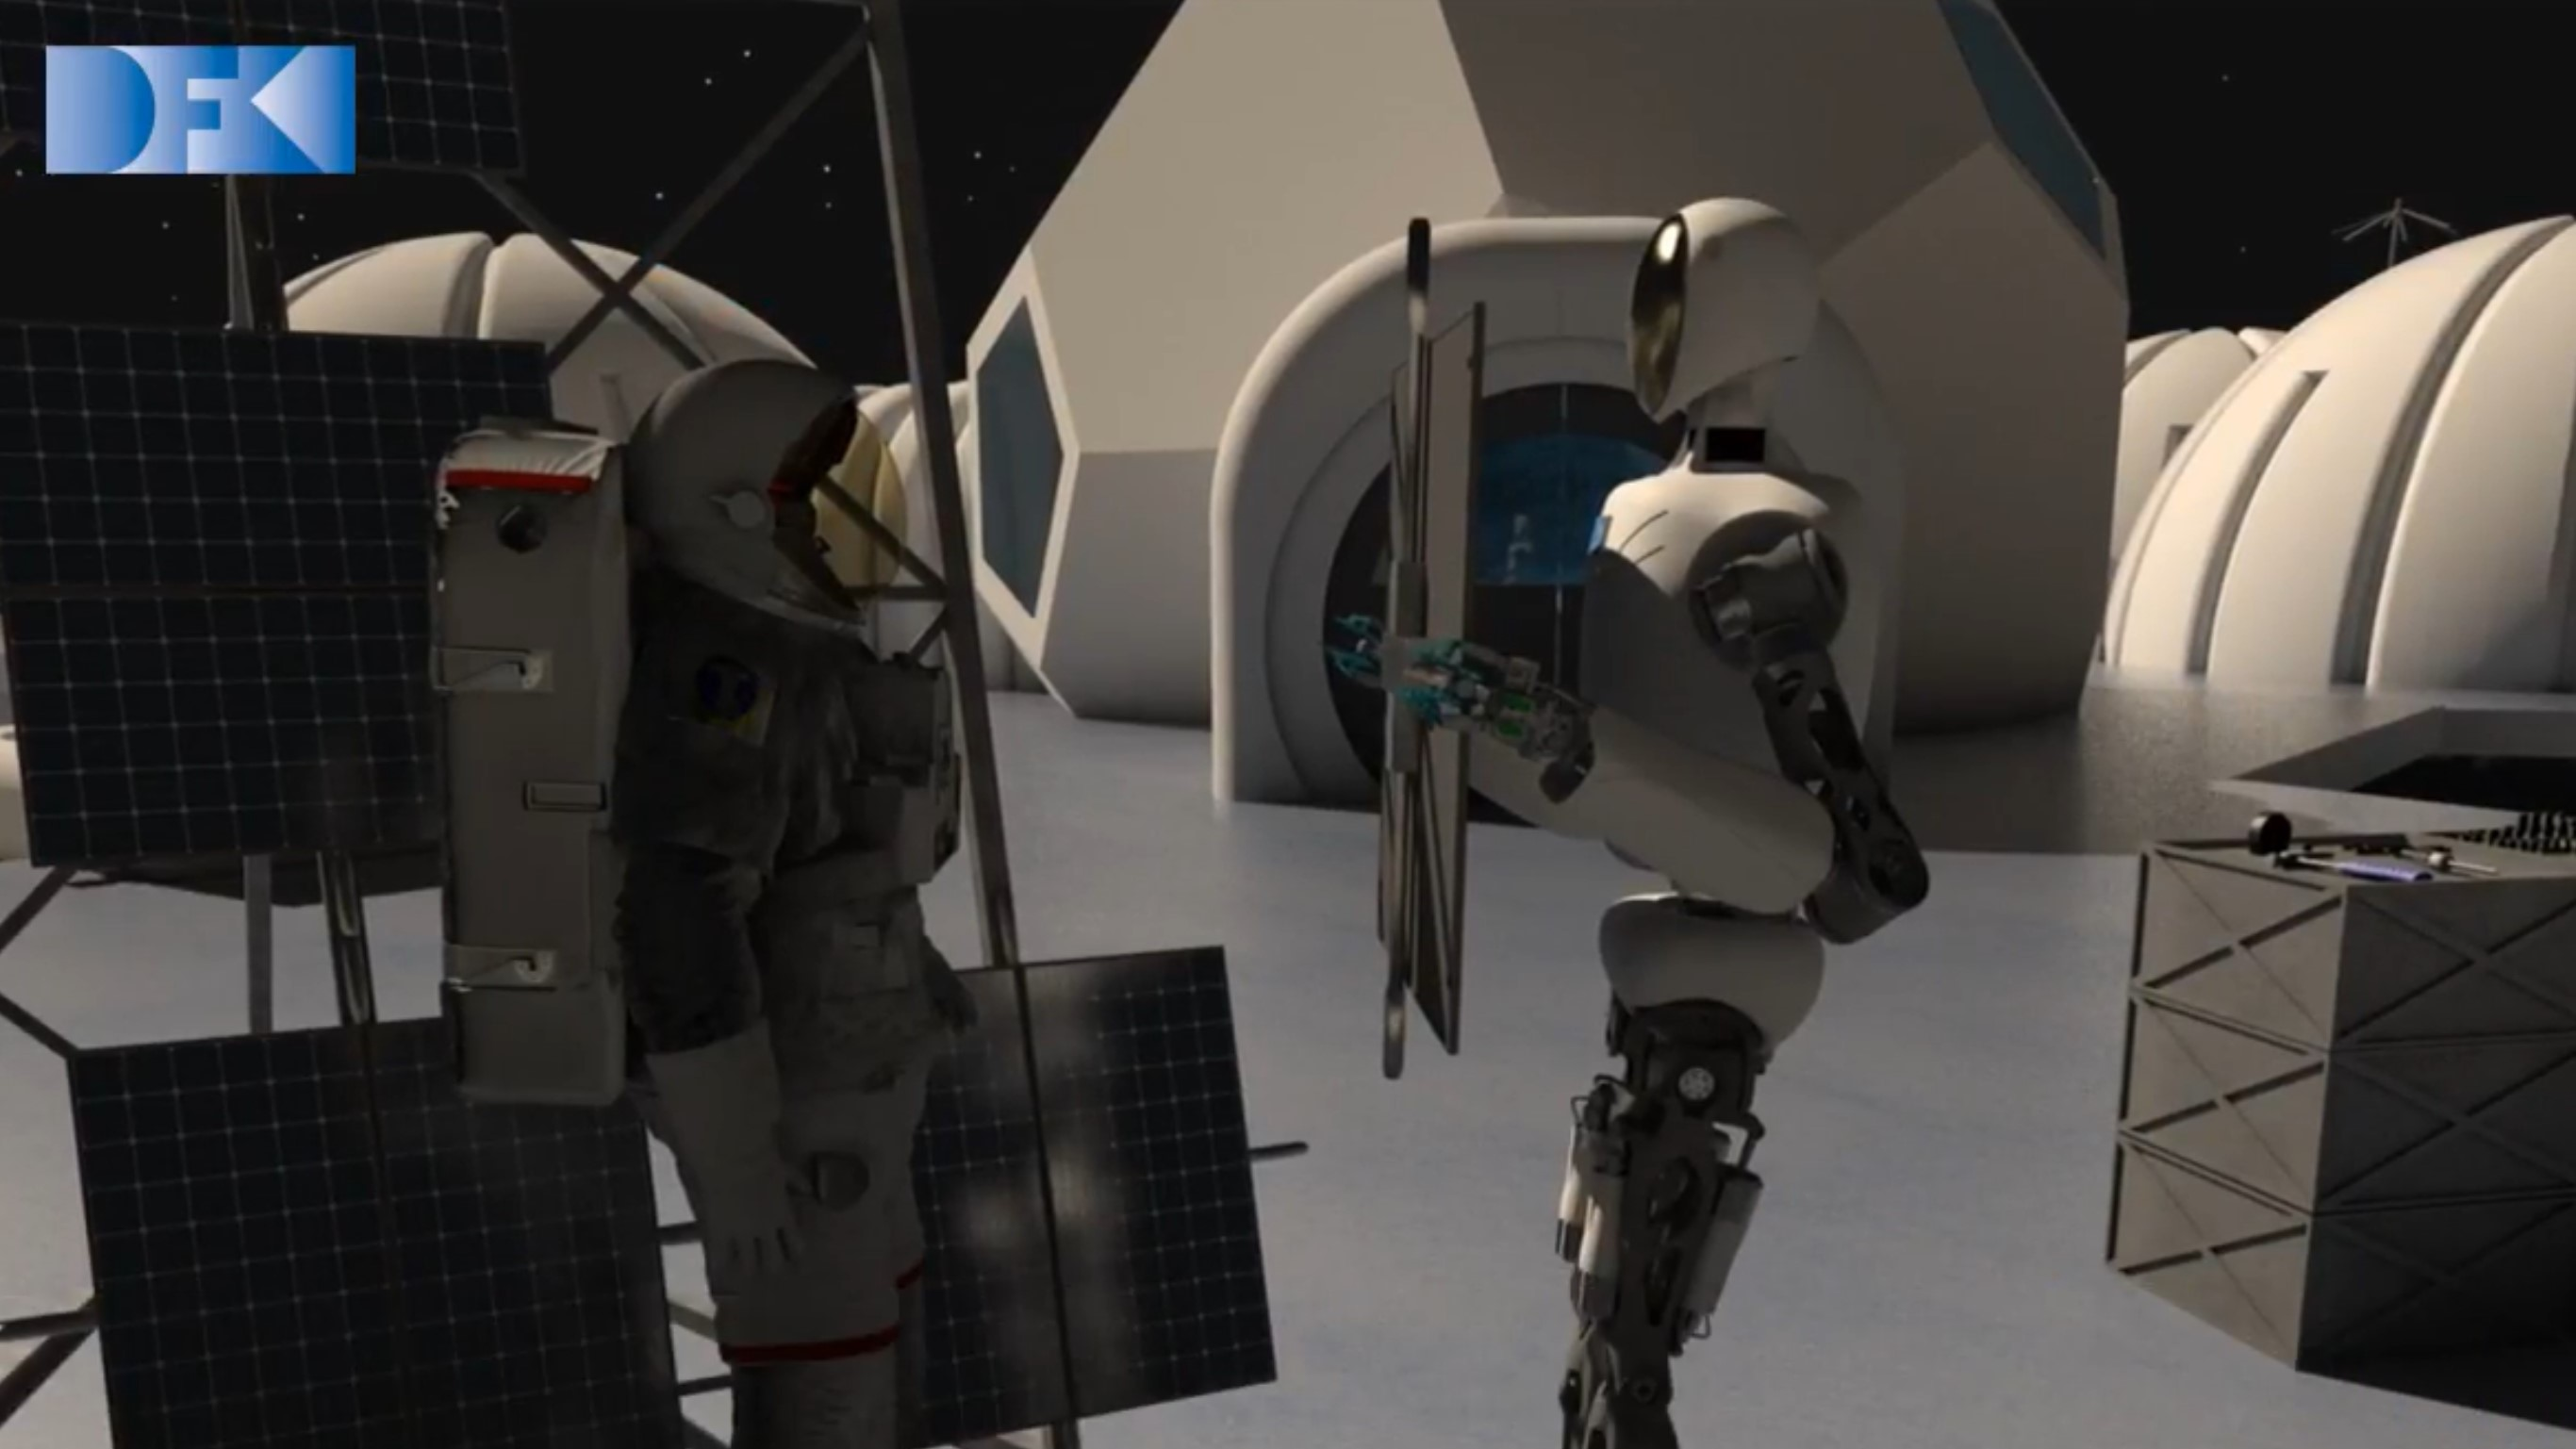
\includegraphics[width=.7\textwidth]{img/intro/rh5_interactive_16_9}
\caption[Humanoid robots interact intuitively with humans]{Humanoid robots can interact with humans in a very intuitive manner since they share similar kinematics, sensing and behavior. This opens up new opportunities for the cooperation needed, e.g. when assembling and installing infrastructure on foreign planets \cite{img:rh5_interactive}.}
\label{img:rh5_interactive}
\end{figure} 
    
We perform all these tasks seemingly effortless. But compared to current robots, the dynamic capabilities of humans and animals are still outstanding in terms of versatility, speed, efficiency and robustness \cite{hutter2012starleth}. In order to further close the gap between robots and their natural counterparts, current research is driving towards exploiting the natural dynamics of robots. This implies mutually dependent changes about how we think about the robots design \cite{pratt2004series} on the one hand and about ways of controlling them, on the other hand, in order to move in a more dynamic, efficient and natural way \cite{collins2005efficient, haddadin2012optimal, pratt2000exploiting}.
%\begin{figure}[t]
%	\begin{subfigure}{.5\textwidth}
%		\centering
%		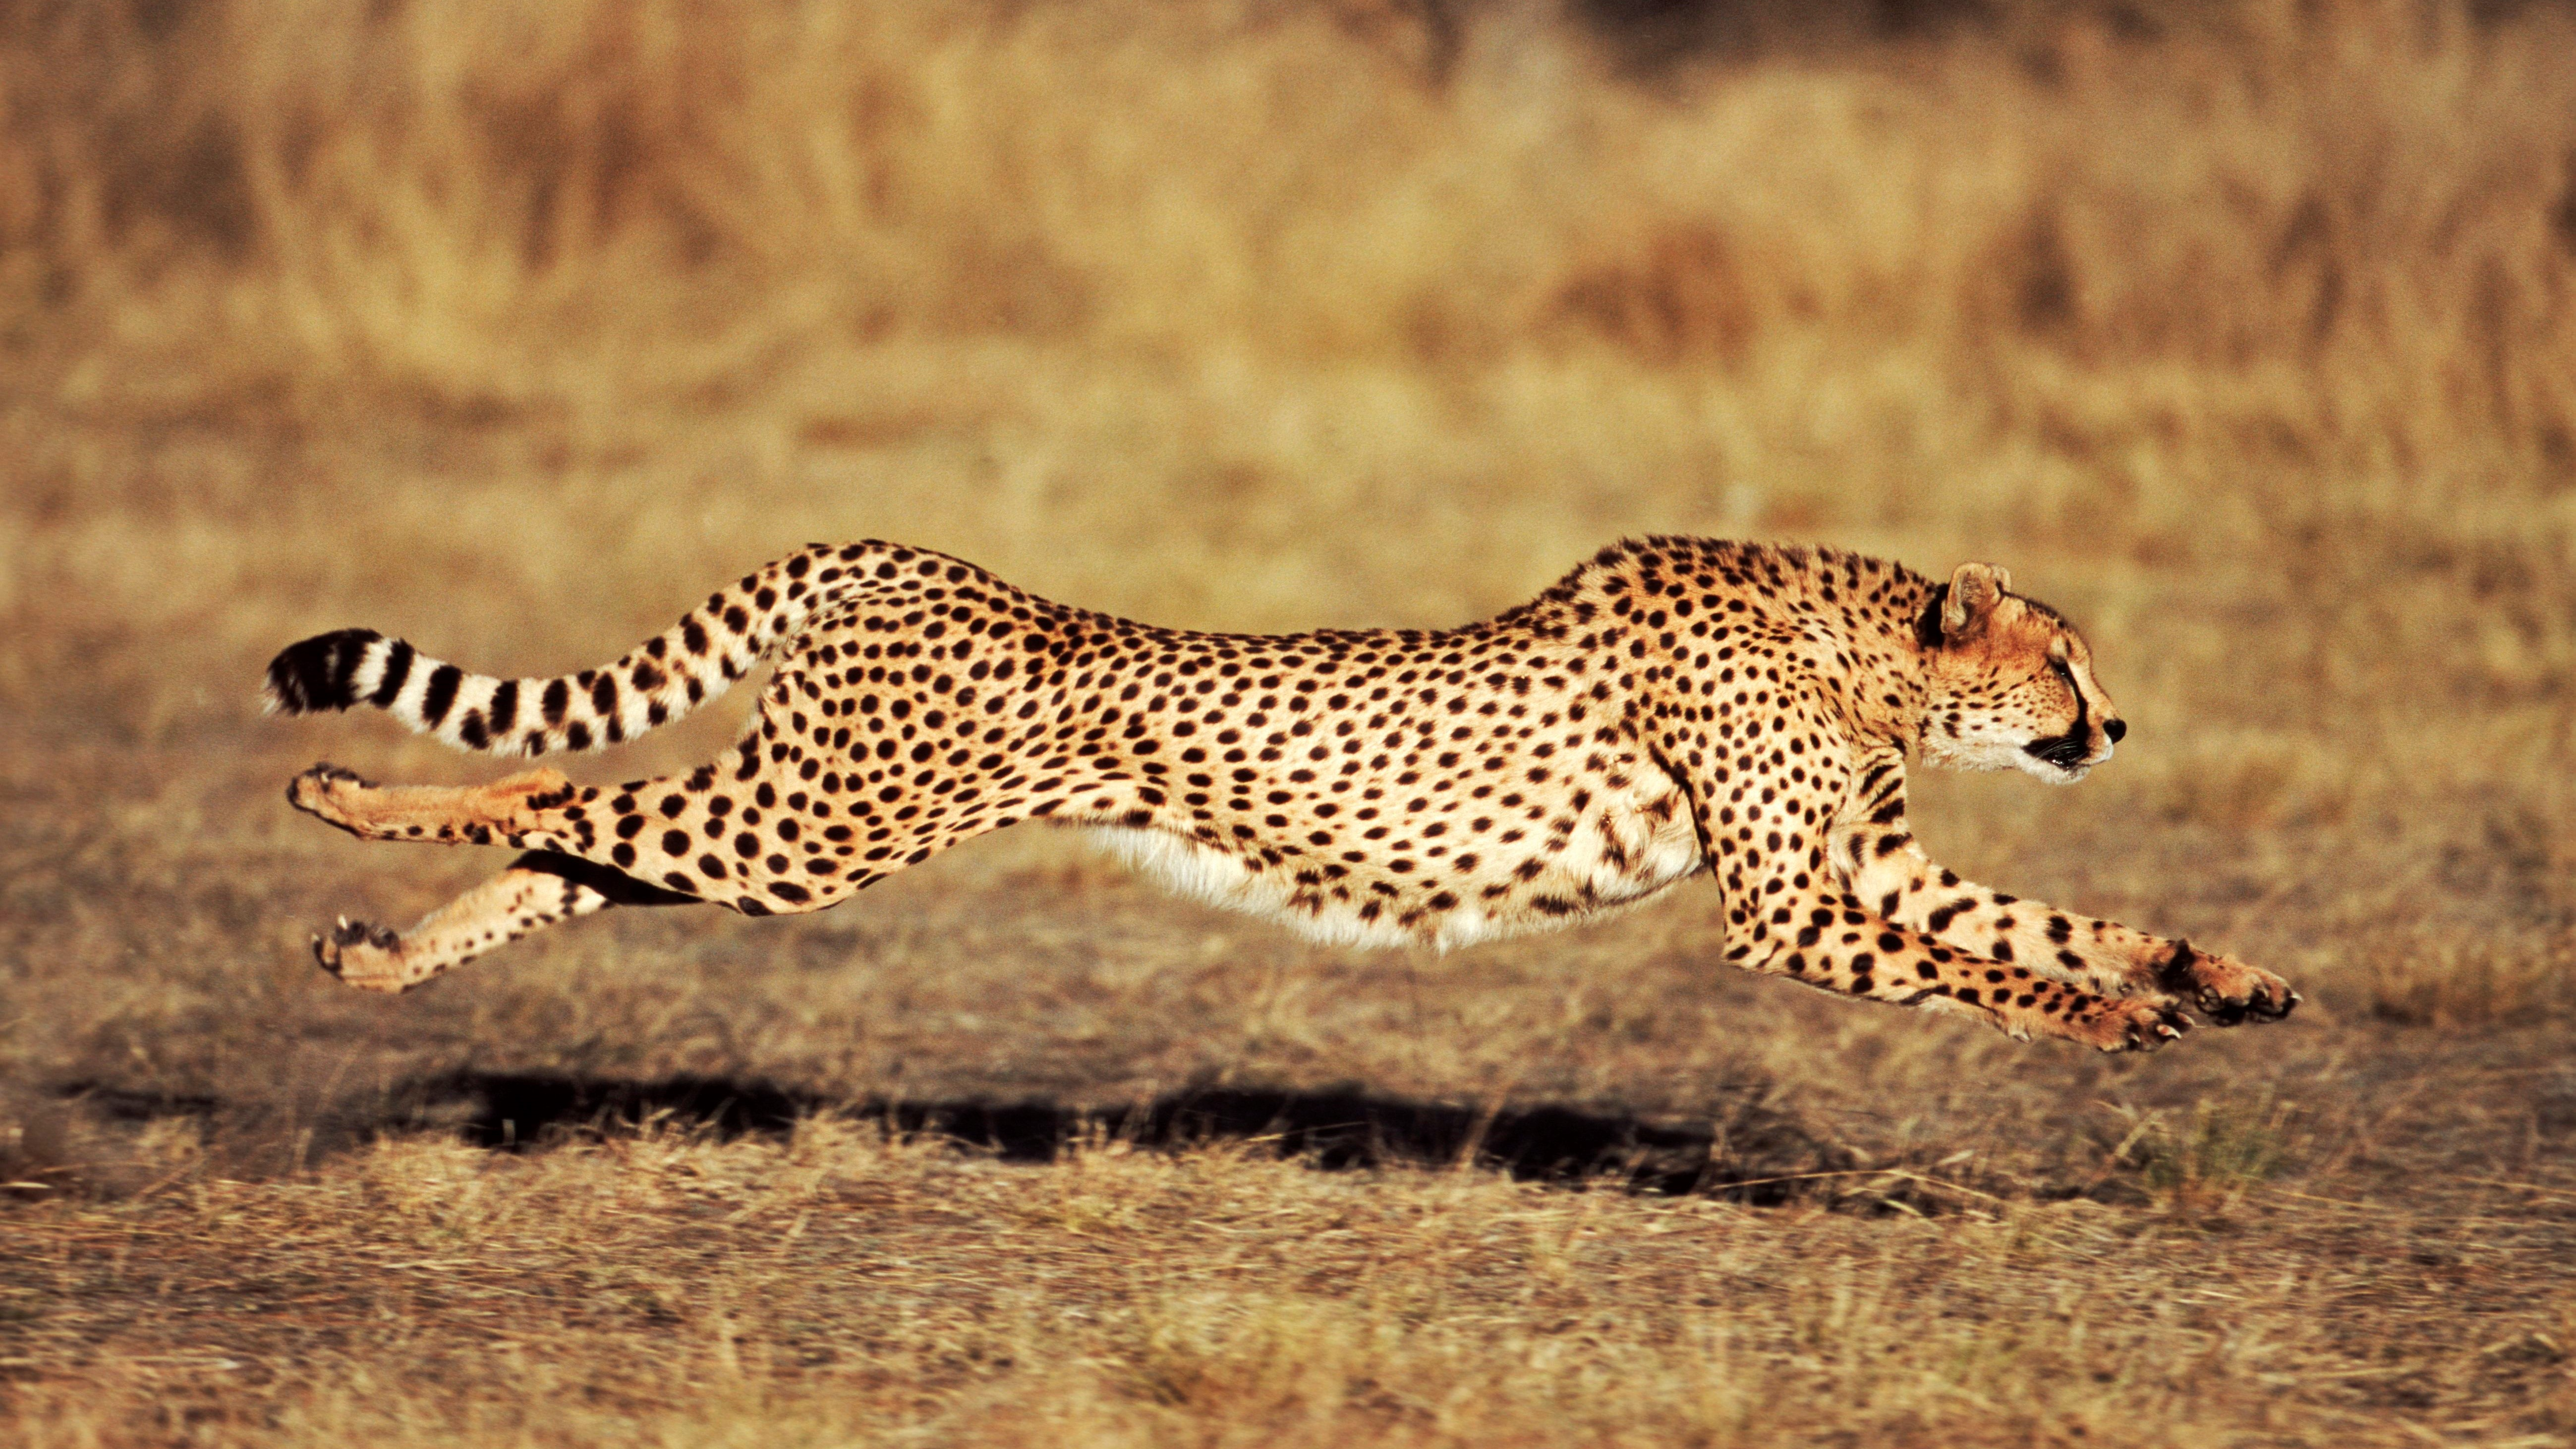
\includegraphics[width=.95\linewidth]{img/cheetah_run_16_9}
%		\caption{Animal in dynamic movement \cite{img:cheetah_run}}
%		\label{fig:animal}
%	\end{subfigure}%
%	\begin{subfigure}{.5\textwidth}
%		\centering
%		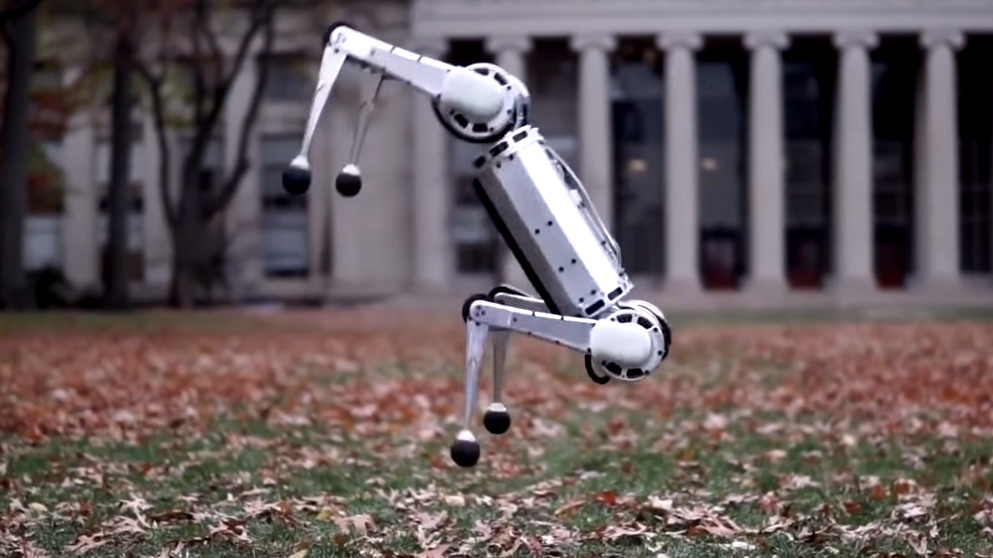
\includegraphics[width=.95\linewidth]{img/mini_cheetah_16_9}
%		\caption{Quadruped Robot Mini Cheetah \cite{img:mini_cheetah}}
%		\label{fig:bert}
%	\end{subfigure}
%	\caption[Quadrupedal locomotion of robots and their biological counterparts.]{Animals and humans combine versatility, speed robustness and efficiency in perfection when moving in rough terrain (a). While important issues in making legged robots (b) move performantly already have been addressed, energy efficiency is one of the major drawbacks in comparison to their biological counterparts.}
%	\label{fig:natural2robot}
%\end{figure}

The specific difficulty of creating bipedal walking motions has several causes. The first difficulty is due to the mechanism complexity, i.e. dealing with high-dimensional degrees of freedom, leading to potentially expensive computations. Secondly, legged locomotion is subject to different contact situations and impact collisions, resulting in multi-phase models and hence hybrid dynamics. Finally, bipeds face the problem of effective underactuation, further restricting the applicable control approaches.

\textit{Dynamic} bipedal locomotion adds additional complexity to this problem. A central characteristic of walking dynamically is that the \gls{CoM} partially leaves the biped's support polygon. Furthermore, there is the need of generating feasible, controllable limit cycles. When considering running motions, difficulties are faced regarding the conservation of angular momentum, which implies restrictions on the controllability during flight phases \cite{westervelt2018feedback}. 


\section{Related Work}\label{sec:IntroRelated}
There are existing different ways to generate feasible motion plans for robotic systems. Common approaches are relying on simplified dynamic models, while recent ones make use of numerical optimization for generating efficient motion plans. 

\subsection{Traditional Legged Locomotion Planning}
Previously we already discovered, why locomotion synthesis for legged robots is a challenging problem. Solving this global problem typically is approached by splitting it up into successive subproblems that are solved sequentially: (i) contact planner, (ii) centroidal pattern generator, (iii) whole-body motion generator (\cref{img:traditional_locomotion_planner}) \cite{carpentier2017multi}. 

\begin{figure}
\centering	
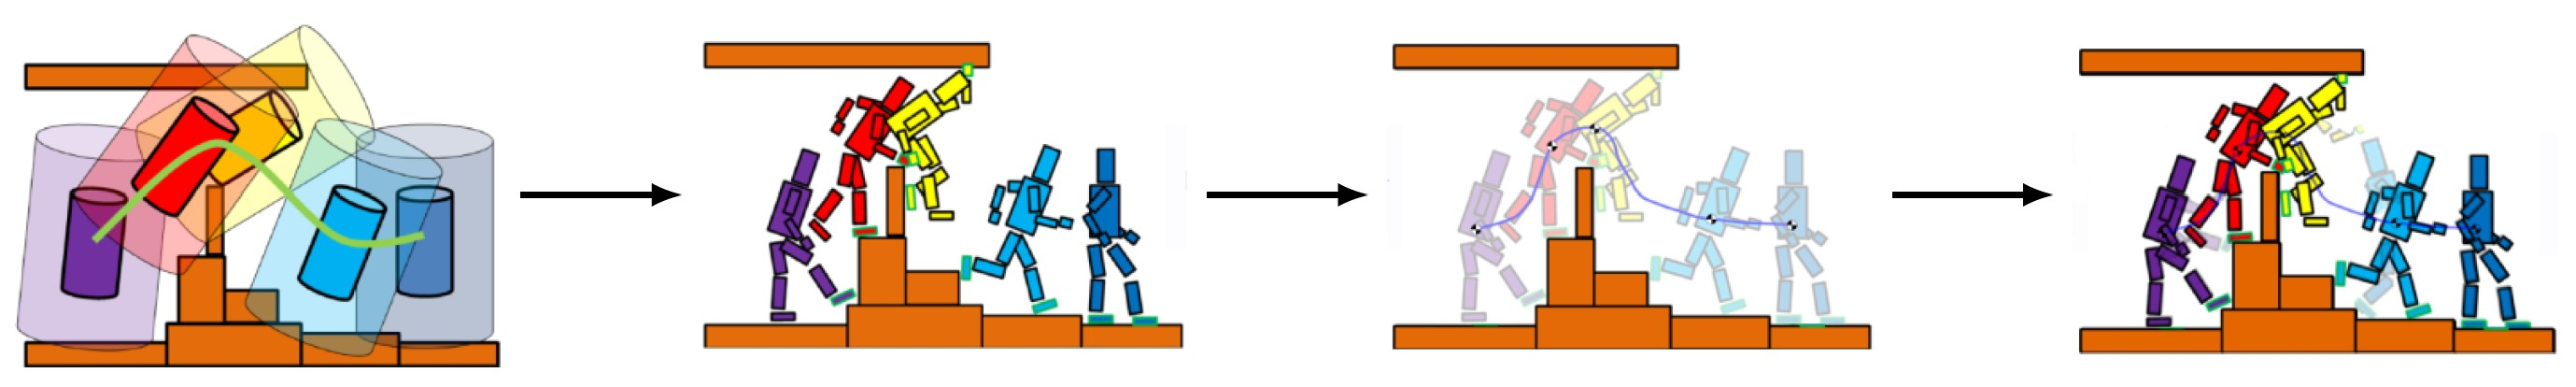
\includegraphics[width=1\textwidth]{img/intro/traditional_locomotion_planner}
\caption[Traditional Legged Locomotion Planning]{Traditional Legged Locomotion Planning \cite{giraud2020motion}. The motion planning problem decomposed into subproblems that are solved sequentially: first, a contact planner solves for feasible foothold positions, then a feasible base motion is generated and finally a consistent whole-body trajectory is derived.}
\label{img:traditional_locomotion_planner}
\end{figure} 
 
The first stage of traditional legged locomotion planning is a contact planner that selects appropriate foothold position and step timings. In other words, this component predefines \textit{where} and \textit{when} external forces can act on the system. 
Once these force locations have been predetermined, the goal is to generate a body motion, i.e. a \gls{CoM} and end-effector trajectories, which can be created with the available forces. A common approach is to model the robot as a \gls{LIP} and find a motion where the \gls{CoP} remains inside the \gls{SP}. The \gls{LIP} can be solved analytically and efficiently and consequently has been used in a variety of approaches \cite{kajita2003biped, kalakrishnan2010fast, winkler2015planning, bellicoso2017dynamic}. 
From the contact sequence and the centroidal trajectory, a dynamic-physical whole-body trajectory has to be found. This often is done by solving the \gls{IK} \cite{espiau1992new} or operational-space \gls{ID} \cite{khatib1987unified} of the system and produces appropriate joint positions or torques, respectively that can be applied to a physical system.

This approach is beneficial in terms of computation time but comes at the cost of limited motion complexity and energy efficiency. 
The first limitation comes from the underlying assumptions of the \gls{LIP} model. More complex motions and terrains might require to place feet at different heights, reorientation of the base or jumping vertically \cite{winkler2018optimization}. Another limitation arises from the fact that whole-body planning produces more efficient motions than a simple program such as an \gls{IK} solver \cite{budhiraja2018differential}.   

\subsection{Trajectory Optimization}
Generating motion plans for dynamic systems is subject to \gls{TO} algorithms that belong to the broader research field of \gls{OC}. 

\gls{TO} is a numerical optimization technique with the goal of finding a state-control sequence, which locally minimizes a predefined cost function given a set of constraints. The approach allows to specify the behavior of a robot directly in the task space, e.g. a desired end-effector trajectory, while reducing the amount of hand-crafted components. 

There are existing different methods to formulate a \gls{TO}, namely \textit{direct} and \textit{indirect} methods. Unlike \textit{direct} methods which explicitly represent the state, \textit{indirect} methods only represent the control inputs while the state is obtained from forward simulation of the system. In direct methods, the \gls{OC} problem is transcribed into a \gls{SQP}, which easily handles both equality and inequality constraints and is implemented in generic off-the-shelf solvers. Consequently, the direct approaches are forced to search in a constrained optimization space which is slower but finds better optima. The indirect approaches are more sensitive to local minima but are faster and better suited for warm-starting. For a comprehensive overview and further information on \gls{TO} methods see \cite{betts1998survey, kelly2017transcription, tassa2014control}.

\gls{TO} based on reduced centroidal dynamics \cite{orin2013centroidal} has become a popular approach in the legged robotics community. In some approaches it is used after planning the contacts \cite{dai2014whole, carpentier2016versatile, herzog2015trajectory} while other approaches simultaneously optimize the centroidal trajectory and the contacts \cite{mastalli2017trajectory, winkler2018gait, aceituno2017simultaneous}. Either way, the transfer from centroidal to whole-body dynamics is only achieved by instantaneous feedback linearization, where typically quadratic programs with task-space dynamics are solved \cite{saab2013dynamic, herzog2016momentum, vaillant2016multi}. 

While \gls{TO} based on reduced dynamics models has shown great experimental results, whole-body \gls{TO} instead is proven to produce more efficient motions, with lower forces and impacts \cite{budhiraja2018differential}. Hence, we will focus on \textit{indirect methods}, namely \gls{DDP} to compute the whole-body motion. \gls{DDP} allows to efficiently solve nonlinear \gls{OC} problems due to its intrinsic sparse structure and is introduced in \crefrange{sec:TheoryDDP}{sec:TheoryConstrainedDDP} in more detail.

\subsection{Crocoddyl Framework} 
\href{https://github.com/loco-3d/crocoddyl#contact-robot-control-by-differential-dynamic-programming-library-crocoddyl}{Crocoddyl} (Contact RObot COntrol by Differential Dynamic Library) is a recently presented open-source framework for efficient multi-contact optimal control \cite{mastalli20crocoddyl}, which is used within this thesis to plan whole-body motions. 

The framework allows to efficiently compute optimal robot trajectories with predefined contact phases. Its solver is based on various efficient \gls{DDP}-like algorithms. Along with Crocoddyl, a novel optimal control algorithm called \gls{FDDP} is introduced. The \gls{FDDP} algorithm is an improved version of the classical \gls{DDP} algorithm, which shows a greater globalization strategy. In the scope of this thesis all presented \gls{OC} problems are solved with the \gls{FDDP} algorithm with box-constraints on the control inputs.
%The framework can be used in one of two ways: either offline, where a stabilizing controller is built around the nominal trajectory or in a \gls{MPC} sense, where the optimal trajectory is (re-)computed online. 

Crocoddyl allows the computation of highly-dynamic movements (e.g. jumping, front-flip) within few milliseconds. However, these exemplary case studies do not produce balanced motions, leading to motion plans that are hard to stabilize on a real system \cite{giraud2020motion}. To this end, we present a generic method for constraining DDP-like solvers in order to generate inherently balanced, dynamic motions that are applicable on real robots (see \cref{c3}).    

\subsection{RH5 Humanoid Robot}\label{subsec:RH5}
The derived motion planning approach (see \cref{c3}) has been tested both in simulation and real-world experiments on a full-size humanoid robot (see \crefrange{c4}{c6}. RH5 is a lightweight and biologically inspired humanoid that has recently been developed at DFKI Robotics Innovation Center \cite{peters2017konstruktion}.

The RH5 humanoid robot (see \cref{img:rh5_robot}) is designed to mimic the human anatomy with a total size of 200 cm, a weight of 62 kg and a total of 32 \gls{DoF}. The two legs account for 12 \gls{DoF}, the torso and neck kinematics each for three and the arms and grippers of the robot for 14 \gls{DoF}. In order to achieve a dynamic walking speed of 1 m/s, the robot's design follows a series-parallel hybrid approach \cite[Ch.2]{kumar2019modular}. Consequently, linkages and parallel mechanisms are utilized in most of the robot's joints, e.g. the hip-flexion-extension, knee, ankle, torso and wrist. A comparison of RH5 with other state of the art humanoid robots revealed several advantages of this design approach, including increased maximum velocity and torque of the ankle as well as an advantageous weight of the lower leg \cite{kumar2020survey}. Within the analysis of the motion planning approach, the maximum performance of the robot is evaluated in several case studies of highly-dynamic movements (see \cref{c5}).

\begin{figure}[h!]
\centering	
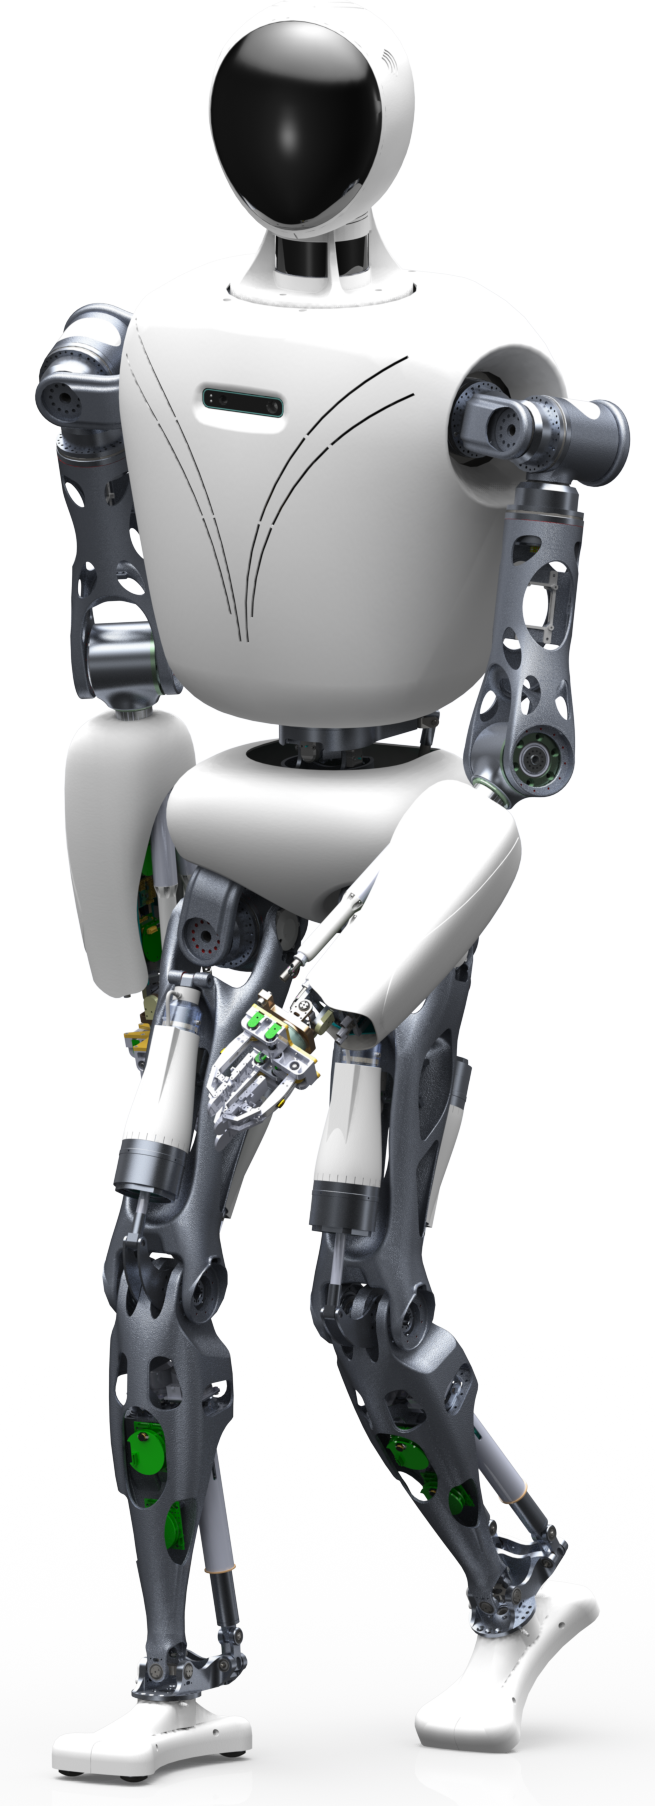
\includegraphics[width=.17\textwidth]{img/intro/rh5_robot}
\caption[The lightweight and biologically inspired humanoid RH5]{The recently presented RH5 is a lightweight and biologically inspired humanoid used as experimental platform within this thesis.}
\label{img:rh5_robot}
\end{figure} 


\section{Contributions}\label{sec:IntroContributions}
The overall goal of this master's thesis is to contribute to the research field of humanoid robotics by applying, evaluating and extending recently presented whole-body \gls{TO} approaches on the RH5 humanoid robot. 

The proposed motion planning approach (see \cref{img:approach}) consists of a DDP-based whole-body \gls{TO}. 
Beneath the contact position and timings, it also considers a set of contact stability constraints that allow computing inherently balanced motions. Output of the \gls{OC} problem is a feasible state trajectory $\myM{X}^*$ with according optimal control inputs $\myM{U}^*$. In contrast to many other motion planning concepts followed by the legged robotics community, our approach (i) considers the full robot dynamics instead of using a reduced dynamics model such as the \gls{LIP} model and (ii) simultaneously optimizes for the centroidal motion, contact stability and whole-body trajectory instead of a sequential optimization. 

\begin{figure}
\centering	
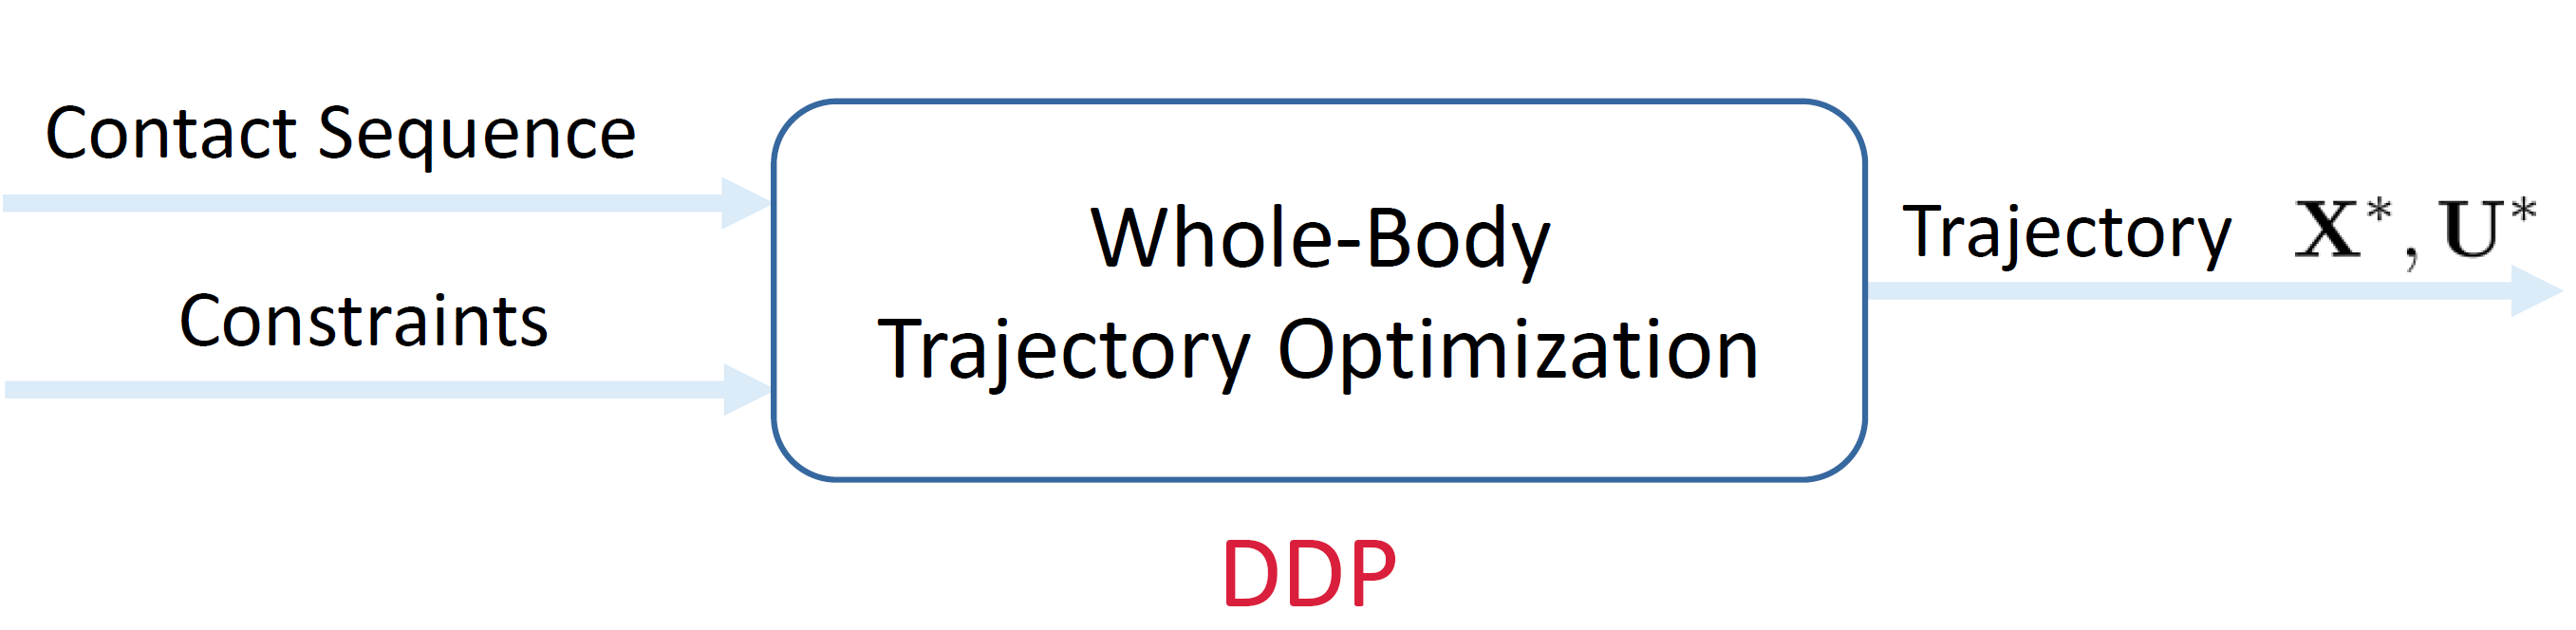
\includegraphics[width=.8\textwidth]{img/approach}
\caption[Overall motion planning approach proposed within this thesis]{The motion planning approach proposed within this thesis. Based on predefined foothold positions, step timings and stability constraints a \gls{DDP}-based whole-body \gls{TO} is used to generate inherently balanced motion plans.}
\label{img:approach}
\end{figure}

The specific contributions of this thesis are summarized below.

\paragraph{C1.} A method for constraining DDP-like solvers in order to generate inherently balanced dynamic motions. The results are integrated into the open-source framework Crocoddyl.
\paragraph{C2.} Evaluation of the stability of the proposed motion planning approach for bipedal walking gaits of increasing complexity in simulation.
\paragraph{C3.} An experimental pipeline for executing optimization-based whole-body motions on a series-parallel hybrid robot.
\paragraph{C4.} Identification of physical limitations for the RH5 humanoid by performing highly-dynamic movements as basis for future design iterations.   

\section{Structure}
This thesis is organized in a total of 7 chapters. 
%Fig. XXX shows the overall outline of this thesis. 
In the following, a summary of each chapter is provided which allows the readers to easily navigate through this document.

\begin{figure}
\centering	
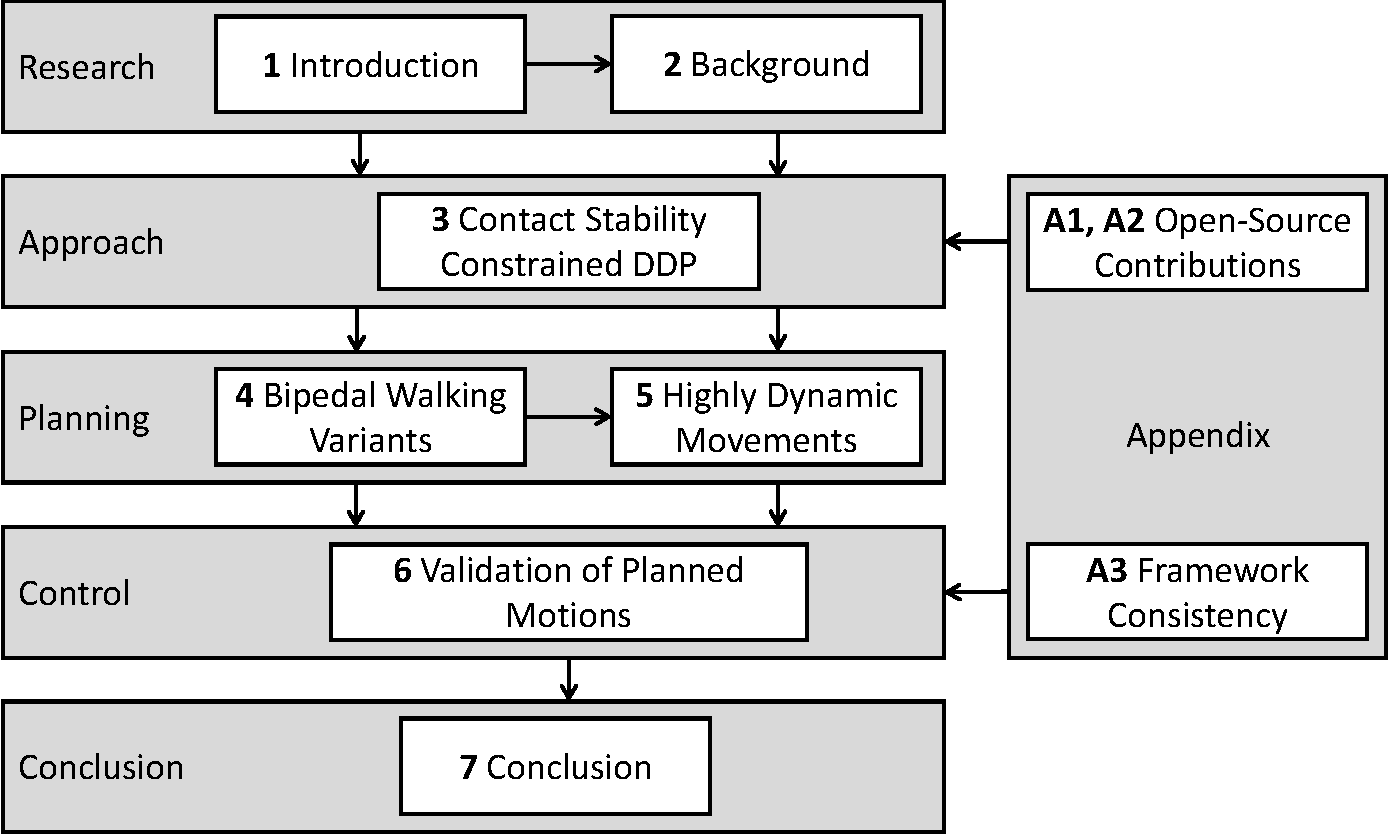
\includegraphics[width=.8\textwidth]{img/structure3}
\caption[Thesis structure and interconnection of chapters]{Thesis structure and interconnection of chapters.}
\label{img:structure}
\end{figure}

\paragraph{\hyperref[c1]{Chapter 1 (Introduction)}} motivates the problem and presents the related work and specific contributions. It also provides details on the structure of the thesis.
\paragraph{\hyperref[c2]{Chapter 2 (Mathematical Background)}} provides the reader with fundamental background in bipedal locomotion and stability analysis. Furthermore, it introduces the class of algorithms and relevant extensions used in this work.
\paragraph{\hyperref[c3]{Chapter 3 (Contact Stability Constrained DDP)}} presents a generic method for integrating stability constraints into DDP-like solvers in order to generate inherently balanced dynamic motions.
\paragraph{\hyperref[c4]{Chapter 4 (Bipedal Walking Variants)}} studies the proposed motion planning approach for bipedal walking gaits of increasing complexity and evaluates the resulting contact stability. 
\paragraph{\hyperref[c5]{Chapter 5 (Highly-Dynamic Movements)}} studies the proposed motion planning approach for highly-dynamic movements and evaluates the performance limits of the RH5 humanoid robot.
\paragraph{\hyperref[c6]{Chapter 6 (Validation of Planned Motions)}} validates the physical correctness of the planned motions by stabilizing the \gls{OC} trajectories with a simple control architecture in a real-time physics simulation and in real-world experiments.
\paragraph{\hyperref[c7]{Chapter 7 (Conclusion and Outlook)}} presents the summary of the thesis and identifies future research directions. 
\paragraph{\hyperref[app:ContactCoP]{Appendix A.1, A.2 (Open-Source Contributions)}} contains the implementation of the \gls{CoP} costs for contact and impulse dynamics, integrated into the open-source framework Crocoddyl within the scope of this thesis. 
\paragraph{\hyperref[app:Consistency]{Appendix A.3 (Framework Consistency)}} provides a proof for consistency between the used frameworks \href{https://github.com/stack-of-tasks/pinocchio}{Pinocchio}, \href{https://github.com/loco-3d/crocoddyl#contact-robot-control-by-differential-dynamic-programming-library-crocoddyl}{Crocoddyl} and \href{https://robotik.dfki-bremen.de/en/research/softwaretools/hyrodyn/}{HyRoDyn}. 






















%%-----------------------------------------------------------------------------%
%                                                                             %
%    K A P I T E L   3                                                      %
%                                                                             %
%-----------------------------------------------------------------------------%

\chapter{Contact Stability Constrained DDP}\label{c3}
This chapter presents a generic method for integrating contact stability constraints into DDP-like solvers. The key idea is to define inequality constraints for unilaterality, friction and the \gls{CoP} of each contact surface with the goal of generating inherently balanced motions.

\section{The Idea}\label{sec:StabilityIdea}
Stability of the contacts is an essential objective of motion planning since prevents the robot from sliding and falling down. In \cref{sec:TheoryStability} we have explored two different criteria for ensuring contact stability for dynamic systems, namely the \gls{ZMP} and \gls{CoP}. As outlined, the application of the \gls{ZMP} is limited due to the assumptions of sufficiently high friction and the existence of one planar contact surface. Since we want to provide a \textit{generic} method that can also be used for e.g. walking up stairs, these simplifying assumptions do not hold anymore. 

Consequently, we decide to model a 6D surface contact, as introduced in \cref{eqn:EoMLeggedRobotSurfaceContact} with dedicated constraints for (i) unilaterality of the contact forces (ii) Coulomb friction on the resultant force, and (iii) \gls{CoP} inside the support area. For the sake of simplicity, we model a rectangular contact area. Nevertheless, this concept can be extended  to arbitrary feet designs. This approach can be compared to the concept of contact wrench cone \cite{caron2015stability}, without additionally enforcing the yaw torque constraint. These inequality constraints for surface contacts can compactly be summarized as
\begin{subequations}\label{eqn:contractWrenchConeReduced}
\begin{align}
f_i^z &> 0 \label{subeqn:stabilityUnilaterality},\\
\mid f_i^x\mid &\leq \mu f_i^z \label{subeqn:stabilityFrictionX},\\
\mid f_i^y\mid &\leq \mu f_i^z \label{subeqn:stabilityFrictionY},\\
\mid X\mid & \geq C_x \label{subeqn:stabilityCoPPitch},\\
\mid Y\mid & \geq C_y \label{subeqn:stabilityCoPRoll}.
\end{align}
\end{subequations}
%Original CoP constraints from Caron paper for horizontal floor
%\mid \tau_i^x\mid & \leq Yf_i^z \label{subeqn:stabilityCoPPitch},\\
%\mid \tau_i^y\mid & \leq Xf_i^z \label{subeqn:stabilityCoPRoll}.

Let us now detail each line of the approach. 
The first inequality \cref{subeqn:stabilityUnilaterality} accounts for the unilaterality of the contact force. By nature, contact forces always have to be positive since the robot can only \textit{push} from the ground, not \textit{pull} to the ground (\cref{img:simple_contact}). 
Inequality \cref{subeqn:stabilityFrictionX,subeqn:stabilityFrictionY} corresponds to the Coulomb friction, where $\mu$ denotes the static coefficient of friction. From a modeling perspective, this can be interpreted via the concept of spatial friction cones \cite{kao2016contact}. If, and only if the distributed contact forces lie inside their respective friction cones, these constraints are satisfied. 
Finally, inequality \cref{subeqn:stabilityCoPPitch,subeqn:stabilityCoPRoll} constrain the \gls{CoP} to lie inside the rectangular contact area of each foot (see \cref{img:contact_surface}). $C_x$ and $C_y$ denote the x and y position of $\bp_{CoP}$, respectively. These \gls{CoP} constraints prevent the robot from tilting around the edges of the rectangular surface contact. In particular, \cref{subeqn:stabilityCoPPitch} corresponds to a constraint of tilting around the pitch axis and \cref{subeqn:stabilityCoPRoll} prevents tilting around the roll axis.

Both, the unilaterality of the contact forces and the friction cone constraints, are already implemented inside Crocoddyl. However, the central component, bounding the \gls{CoP} to lie inside the support area of each contact foot, is missing. Therefore, the rest of this chapter deals with the derivation of a set of implementable \gls{CoP} constraints and describes the integration of these constraints as a cost function into the Crocoddyl framework.
\begin{figure}[t]
	\begin{subfigure}{.5\textwidth}
		\centering
		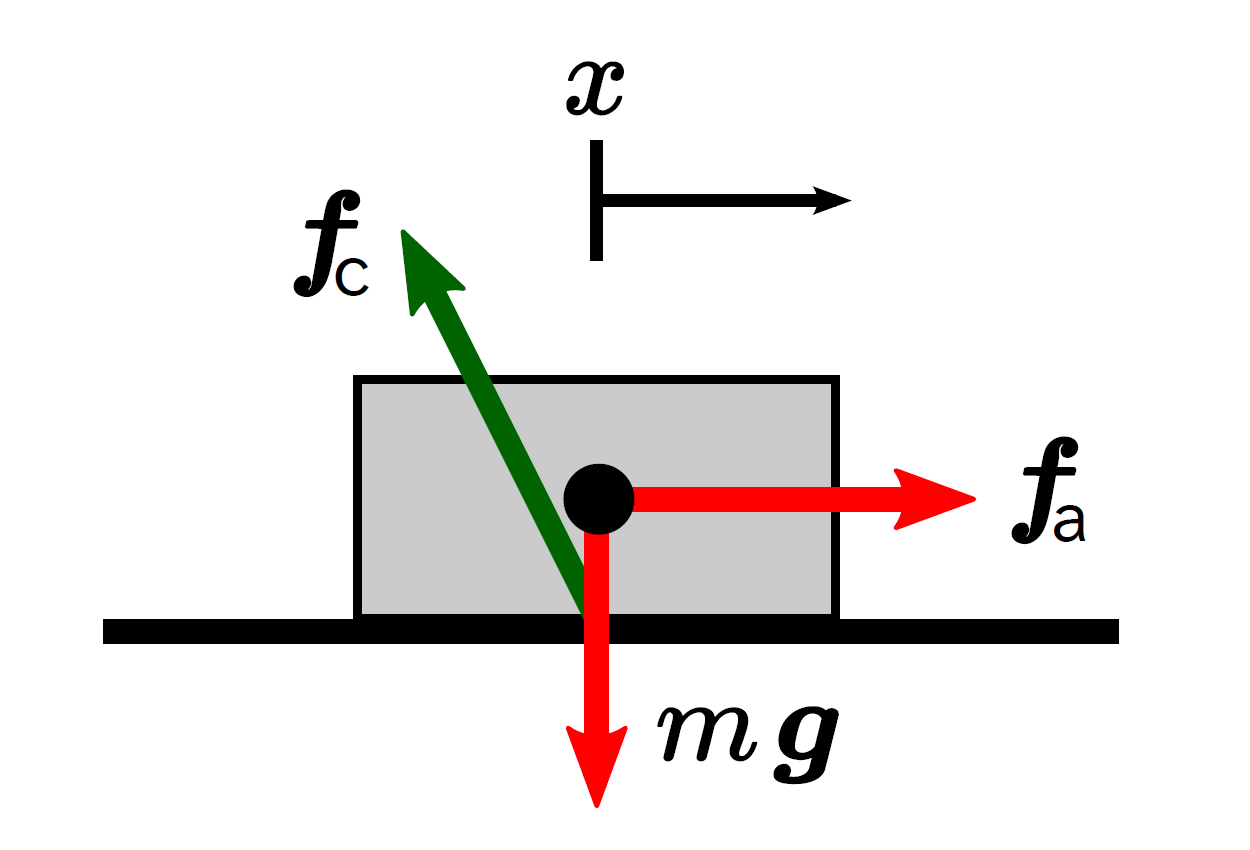
\includegraphics[width=.95\linewidth]{img/simple_contact}
		\caption{}
		\label{img:simple_contact}
	\end{subfigure}%
	\begin{subfigure}{.5\textwidth}
		\centering
		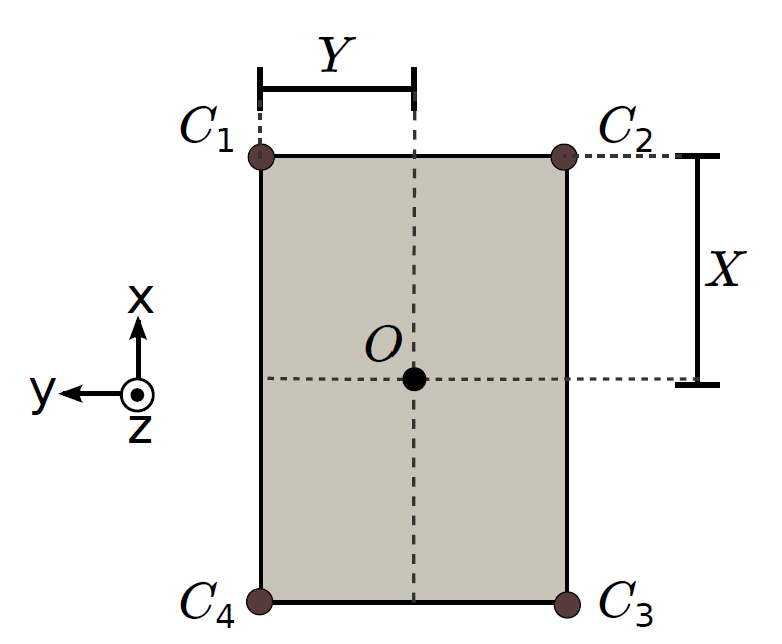
\includegraphics[width=.77\linewidth]{img/contact_surface}
		\caption{}
		\label{img:contact_surface}
	\end{subfigure}
	\caption[Simplified contact situation and CoP notation]{(a) Visualization of acting forces on a simple rigid body and (b) notation used for the \gls{CoP} definition in the contact surface plane \cite{caron2015stability}.}
	\label{fig:natural2robot}
\end{figure}


\section{Center of Pressure (CoP) Constraints}\label{sec:StabilityCoP}
In this section we will derive a universal set of implementable constraints that bound the \gls{CoP} to lie inside the rectangular contact area of each foot.

\subsection{CoP Stability Conditions}
Recapitulate the constraints from inequality \crefrange{subeqn:stabilityCoPPitch}{subeqn:stabilityCoPRoll}. Instead of using the absolute value of $X$ and $Y$, one can also formulate the constraints as
\begin{align}
\begin{split}
-X \leq C_x \leq X,\\
-Y \leq C_y \leq Y.
\end{split}
\end{align}
Based on this formulation it becomes evident that the \gls{CoP} is constrained to lie inside the foot geometry visualized in \cref{img:contact_surface}. In fact, these conditions can be represented via four single inequality equations as
\begin{align}\label{eqn:CoPInequalities}
\begin{split}
X + C_x \geq 0, \\
X - C_x \geq 0, \\
Y + C_y \geq 0, \\
Y - C_y \geq 0. \\
\end{split}
\end{align}
These four inequality equations will be used in the following to formulate the \gls{CoP} constraints.   

\subsection{CoP Computation}
Our goal is to determine explicit expressions for $C_x$ and $C_y$ for arbitrary floor orientations, including inclined ground. To this end, consider the computation routine for the \gls{CoP} from \cref{eqn:CoPComputation}
\begin{equation*} 
\bp_{CoP}=\dfrac{\bn\times\myM{\btau_O^c}}{\bfun^c\cdot\bn}.
\end{equation*}
For arbitrary orientations of the contact normal vector $\bn$, we obtain
\begin{equation}\label{eqn:CoPComputationDetailed}
\bp_{CoP}=\dfrac{\bn\times\myM{\btau_O^c}}{\bfun^c\cdot\bn} = \dfrac{\begin{bmatrix} n_x \\ n_y \\ n_z \end{bmatrix} \times \begin{bmatrix} t_x \\ t_y \\ t_z \end{bmatrix}}{\begin{bmatrix} f_x \\ f_y \\ f_z \end{bmatrix} \cdot \begin{bmatrix} n_x \\ n_y \\ n_z \end{bmatrix}} = 
\begin{bmatrix} n_yt_z - n_zt_y \\ n_zt_x-n_xt_z \\ n_xt_y-n_yt_x \end{bmatrix}\cdot \dfrac{1}{f_xn_x+f_yn_y+f_zn_y},
\end{equation}
and solve for the desired position $C_x$ and $C_y$ of the \gls{CoP} as
\begin{subequations}
\begin{align}
C_x&=\dfrac{n_yt_z - n_zt_y}{f_xn_x+f_yn_y+f_zn_y}, \label{subeqn:Cx}\\
C_y&=\dfrac{n_zt_x-n_xt_z}{f_xn_x+f_yn_y+f_zn_y} \label{subeqn:Cy}.
\end{align}
\end{subequations}

\subsection{CoP Inequality Constraints}
Now that we have found explicit expressions for computing the \gls{CoP} (\crefrange{subeqn:Cx}{subeqn:Cy}), we can insert them into \cref{eqn:CoPInequalities}, which gives a set of four \gls{CoP} constraints as 
\begin{align}\label{eqn:CoPInequalityEqs}
\begin{split}
X + \dfrac{n_yt_z - n_zt_y}{f_xn_x+f_yn_y+f_zn_y} \geq 0, \\
X - \dfrac{n_yt_z - n_zt_y}{f_xn_x+f_yn_y+f_zn_y} \geq 0, \\
Y + \dfrac{n_zt_x-n_xt_z}{f_xn_x+f_yn_y+f_zn_y} \geq 0, \\
Y - \dfrac{n_zt_x-n_xt_z}{f_xn_x+f_yn_y+f_zn_y} \geq 0. \\
\end{split}
\end{align}
These conditions can be written in matrix form as:  
\begin{equation}\label{eqn:CoPInequalityMatrix}
\begin{bmatrix}  
Xn_0 & Xn_1 & Xn_2 & 0 & -n_2 & n_1 \\
Xn_0 & Xn_1 & Xn_2 & 0 & n_2 & -n_1 \\
Yn_0 & Yn_1 & Yn_2 & n_2 & 0 & -n_0 \\
Yn_0 & Yn_1 & Yn_2 & -n_2 & 0 & n_0 \\ \end{bmatrix}
\begin{bmatrix} f^x \\ f^y \\ f^z \\ \tau^x \\ \tau^y \\ \tau^z \end{bmatrix} \geq
\begin{bmatrix} 0 \\ 0 \\ 0 \\ 0 \end{bmatrix},
\end{equation}
and finally yield an implementable set of inequality equations for constraining the \gls{CoP} to lie inside the rectangular contact area of each foot. 


\section{Integration Into the Crocoddyl Framework}\label{sec:StabilityIntegration}
This section presents the integration of the derived CoP inequality constraints from \cref{eqn:CoPInequalityMatrix} into the Crocoddyl framework. 

\subsection{Inequality Constraints by Penalization}
In \cref{sec:TheoryConstrainedDDP} we have discussed possible ways of incorporating inequality constraints into DDP-like solvers. Crocoddyl handles inequality constraints, such as joint limits or friction cone, via penalization. 
In numerical optimization, the goal is to minimize a given cost function. In Crocoddyl, an \textit{action model} combines dynamics and cost model for each knot of the discretized \gls{OC} problem from \cref{eqn:totalCost}. The cost function for an action model at knot $n$ can be written as: 
\begin{equation}\label{eqn:costSum}
l_n=\sum_{c=1}^{C}\alpha_c\Phi_c(\bq,\dot{\bq}, \btau), 
\end{equation}
where $C$ different costs $\Phi_c$ are weighted by a respective coefficient $\alpha_c\in R$. The goal of the following two parts is to demonstrate how the inequality \cref{eqn:CoPInequalityMatrix} is implemented inside a novel cost function into the framework.

\subsection{Computation of Residual and Cost}
%\subsection{Computation of the Residual}
In numerical analysis, the term \textit{residual} corresponds to the error of a result \cite{shewchuk1994introduction}. For the sake of compactness, we abbreviate \cref{eqn:CoPInequalityMatrix} as 
\begin{equation} \label{eqn:costPositive}
\myM{A} \myM{w} \geq \myM{0},
\end{equation}
where $\myM{A}$ corresponds to a matrix of \gls{CoP} inequality constraints and $\myM{w}$ is the contact wrench acting on the according foot. The residual $\myM{r}\in \myM{R}_{4\times 1}$ of the cost is retrieved by a simple matrix-vector multiplication:
\begin{equation}\label{eqn:costResidual}
\myM{r} = \myM{A} \myM{w}.
\end{equation} 

%\subsection{Computation of the Cost}
The residual vector depicted in \cref{eqn:costResidual} typically contains non-zero numbers. The resulting scalar \gls{CoP} cost value $\Phi_{CoP}$ is computed via a bounded quadratic activation as
\begin{equation}\label{eqn:CoPCostComputation}
\Phi_{CoP}=
\begin{cases}
\quad\dfrac{1}{2}\myM{r}^T\myM{r} &\mid \text{lb} = \myM{r} = \text{ub} \\[10pt]
\quad 0 &\mid \text{lb} \leq \myM{r} \leq \text{ub}.
\end{cases}
\end{equation}

In order to account for the positiveness of $\myM{r}$ (see \cref{eqn:costPositive}), the bounds are set to $\text{lb}=\myM{0}$ and $\text{ub}=\infty$, respectively. Finally, this bounded quadratic activation of the residual vector has the following implications:
\begin{itemize}
\item The \gls{CoP} cost is zero, whenever $\bp_{CoP}$ lies inside or on the border of the foot area spanned by $X$ and $Y$.
\item The \gls{CoP} cost increases in a quadratic manner, when $\bp_{CoP}$ exceeds the foot area spanned by $X$ and $Y$.
\end{itemize}  
Besides this formulation of the cost function also other designs are conceivable for the future. For example, the Euclidean distance from the CoP to the coordinate origin could be considered when computing the residual (see  \cref{eqn:CoPCostComputation}).

\subsection{Basic Usage and Contributions}
%\subsection{Basic Usage of the CoP Cost}
The cost function is implemented in C++, but can be accessed via Python bindings for versatile and fast prototyping. In the following, a basic example is provided to demonstrate the interface of the \gls{CoP} cost function to the interested reader.
\begin{verbatim}
# 1. Creating the cost model container
costModel = crocoddyl.CostModelSum(state, actuation.nu)
# 2. Defining the CoP cost
footGeometry = np.array([0.2, 0.08]) # dim [m] of the foot area
CoPCost = crocoddyl.CostModelContactCoPPosition(state, 
crocoddyl.FrameCoPSupport(footId, footGeometry), actuation.nu)
# 3. Adding the CoP cost term with assigned weight to the cost model
costModel.addCost("LF_CoPCost", CoPCost, 1e3)
\end{verbatim}

%\subsection{List of Contributions}
The contributions of this thesis to the open-source framework Crocoddyl are summarized in two main pull requests. The first one, \href{https://github.com/loco-3d/crocoddyl/pull/792}{\#792} contains the basic formulation of the \gls{CoP} cost function for contact dynamics action models (see \cref{app:ContactCoP}). With \href{https://github.com/loco-3d/crocoddyl/pull/830}{\#830}, an additional version of the cost function is implemented for impulse dynamics action models (see \cref{app:ImpulseCoP}).
A functional unit test that checks the cost against numerical differentiation as well as accessible python bindings can be found in the according directory of \cite{crocoddylweb}.


%\subsection{Backup: Friction Cone constraints}
%\begin{align}
%\begin{split}
%\mid\mid f^x\mid\mid &\leq \mu f^z \\
%\mid\mid f^y\mid\mid &\leq \mu f^z \\
%f^z &> 0
%\end{split}
%\end{align}
%For the case of four edges of the linear approximation of the friction cone, the equations become:
%\begin{equation}
%\begin{bmatrix} 1 & 0 & -\mu \\
%-1 & 0 & -\mu \\
%0 & 1 & -\mu \\
%0 & -1 & -\mu \\
%0 & 0 & -\mu \\ \end{bmatrix} \cdot
%\begin{bmatrix} f^x \\ f^y \\ f^z \end{bmatrix} \leq
%\begin{bmatrix} 0 \\ 0 \\ 0 \\ 0 \\ 0 \end{bmatrix}
%\end{equation}

%\subsection{CoP Constraints: Horizontal Floor}
%For the special case of horizontal floor, with the according normal vector $\myM{n}=[0,0,1]$, the \gls{CoP} can be computed with the help of \cref{eqn:CoPComputationDetailed} to 
%\begin{equation}
%\myM{p}_{CoP} = \begin{bmatrix} -t_y/f_z \\ t_x/f_z \\ 0 \end{bmatrix},
%\end{equation}
%which in turn can be represented by four inequality conditions:
%\begin{align}
%\begin{split}
%X-\dfrac{\tau_y}{f_z} &\geq 0, \\
%X+\dfrac{\tau_y}{f_z} &\geq 0, \\
%Y+\dfrac{\tau_x}{f_z} &\geq 0, \\
%Y-\dfrac{\tau_x}{f_z} &\geq 0. \\
%\end{split}
%\end{align}
%These conditions can be transformed into matrix form for the purpose of implementation as
%\begin{equation}
%\begin{bmatrix} 
%0 & 0 & X & 0 & -1 & 0 \\
%0 & 0 & X & 0 & 1 & 0 \\
%0 & 0 & Y & 1 & 0 & 0 \\
%0 & 0 & Y & -1 & 0 & 0 \end{bmatrix} \cdot
%\begin{bmatrix} f^x \\ f^y \\ f^z \\ \tau^x \\ \tau^y \\ \tau^z \end{bmatrix} \geq
%\begin{bmatrix} 0 \\ 0 \\ 0 \\ 0 \end{bmatrix}.
%\end{equation}





%%-----------------------------------------------------------------------------%
%                                                                             %
%    K A P I T E L   4                                                        %
%                                                                             %
%-----------------------------------------------------------------------------%

\chapter{Bipedal Walking Variants}\label{c4}
This chapter studies the proposed motion planning approach for bipedal walking gaits of the full-size humanoid RH5. It starts by describing the individual building blocks of the optimization problem, then discusses the simulation results obtained for increasing gait dynamics and finally provides an evaluation of the contact stability of the dynamic motions.

\section{Formulation of the Optimization Problem}\label{sec:BipedFormulation}
This section gives information about the adopted contact and impact modeling techniques and introduces the constraints used for generating physically consistent walking trajectories. The core formulation is based on the legged gaits described in \cite{mastalli20crocoddyl} but contains various improvements necessary for application on real robots. All motions presented in this chapter are solved for a predefined sequence of contacts and step timings. 
Recapitulating \cref{sec:TheoryDDP}, we formulate the optimization problem as
\begin{equation}\label{eqn:optimizationProblem}
\myM{X}^*,\myM{U}^*= 
\arg\min_{\mathbf{X},\mathbf{U}} l_N(x_N)+\sum_{k=0}^{N-1} \int_{t_k}^{t_k+\Delta t} l(\mathbf{x},\mathbf{u})dt. 
\end{equation}

\subsection{Contact and Impact Modeling}
During a walking motion, the body is always in contact with the ground either in single support, or in double support. In \cref{sec:TheoryConstrainedDDP} we have discovered, how rigid contacts can be expressed as a kinematic constraint on the \gls{EoM} (see \cref{eqn:unconstrainedDynamics}). 
Analogously, one can describe the impulse dynamics
\footnote{Impulse dynamics account for the physical effects that occur at a switch from non-contact to contact condition \cite{featherstone2014rigid}.} 
of a multibody system as
\begin{equation}\label{eqn:ImpulseDynamics}
\left[\begin{matrix}\myM{M} & \myM{J}^{\top}_c \\{\myM{J}_{c}} & \myM{0}\end{matrix}\right] \left[\begin{matrix} \myM{v}^+ \\ -\boldsymbol{\Lambda} \end{matrix}\right] = \left[\begin{matrix} \myM{M}\myM{v}^- \\ -e\myM{J}_c \myM{v}^-\end{matrix}\right],
\end{equation}
where $\boldsymbol{\Lambda}$ is the contact impulse, $\myM{v}^-$ and $\myM{v}^+$ are the generalized velocities before and after the impact and $e\in [0,1]$ is the restitution coefficient that accounts for the elasticity of the collision. For all motions, we use this impulse model to account for the infinitesimal short change in the contact situation. To improve the numerical integration stability, terms defined by Baumgarte Stabilization \cite{baumgarte1972stabilization} are used along with the rigid contact constraint described with \cref{eqn:gaussMinimization}. This numerical stabilization on the constraints can be expressed as:
\begin{equation}\label{eqn:BaumgarteStabilization}
a_0=a_{\lambda(c)}-\alpha M_{\lambda(c)}^{\text{ref}}\ominus M_{\lambda(c)}-\beta v_{\lambda(c)},
\end{equation}
where $a_0$ is the desired acceleration in the constrained space, $v_{\lambda(c)}, a_{\lambda(c)}$ are the spatial velocity and acceleration of the contact $\lambda(c)$, respectively, $M_{\lambda(c)}^{\text{ref}}\ominus M_{\lambda(c)}$ is the inverse composition between the reference contact placement and the current one \cite{mastalli20crocoddyl}. The PD gains $\alpha$ and $\beta$ enable an adequate numerical stabilization of the constraints depending on the dynamics of the movement.

\subsection{Robot Tasks}
Robot tasks, such as grasping and object or performing a step, are an essential goal of motion planning. As outlined in \cref{sec:TheoryConstrainedDDP}, these task-related constraints are considered in the optimization process as regulator functions. In the context of this thesis two tasks are of specific interest, namely the foot tracking and \gls{CoM} tracking. 

\paragraph{Foot Tracking Cost}
In order to perform a symmetric gait (see \cref{sec:TheoryBiped}), the design of dedicated foot trajectories is crucial. We use piecewise-linear functions to describe the swing foot reference trajectory. Deviation from this time-depended reference foot trajectory is highly penalized. The foot tracking cost can be formulated via the squared Euclidean norm (L2 norm) as
\begin{equation*} 
\Phi_{\text{foot}}=\mid\mid \myM{f}(t)-\myM{f}^{\text{ref}}(t)\mid\mid^2_2,
\end{equation*}
where $\myM{f}(t)$ is the actual \gls{CoM} position at time-step $t$ and $\myM{f}^\text{ref}(t)$ is the according reference. Start and end position as well as timings are predefined and combined with a desired step height to shape the desired foot trajectory. 

\paragraph{\Gls{CoM} Tracking Cost}
In bipedal locomotion, the three-dimensional position of the \gls{CoM} of the whole-body turned out to be crucial \cite{carpentier2017centre}. This is especially true for quasi-static motions, where the \gls{FCoM} is used as static stability margin as explained in \cref{sec:TheoryBiped}. Analogously to the foot cost, the \gls{CoM} tracking cost is formulated as
\begin{equation*} 
\Phi_{\text{CoM}}=\mid\mid \myM{c}(t)-\myM{c}^\text{ref}(t)\mid\mid^2_2.
\end{equation*}
In order to account for the static stability in these motions, we perform a dedicated shifting of the \gls{FCoM} to the foot center, before performing the swing-foot task. 
%Additionally, the \gls{CoM} is kept at a constant height to prevent unnecessary forces acting on the base of the body. 

\subsection{Inequality Constraints for Physical Consistency}
Essential demands on physically consistent motion planning are that (i) the robot limits (torque, joints) are considered and (ii) the generated trajectories are inherently balanced. To this end, we consider joint limits, friction cone and the novel \gls{CoP} bound as inequality constraints in our formulation, while torque constraints are covered in the algorithm itself.

\paragraph{Contact Stability Constraints}
As detailed in \cref{c3} with the concept of contact stability constrained \gls{DDP}, we constrain unilaterality, friction and \gls{CoP} for each foot in contact. For the sake of clarity, \cref{eqn:CoPCostComputation} is again recalled as 
\begin{equation*}
\Phi_{\text{CoP}}=
\begin{cases}
\quad\dfrac{1}{2}\myM{r}^T\myM{r} &\mid \text{lb} > \myM{r} > \text{ub} \\[10pt]
\quad 0 &\mid \text{lb} \leq \myM{r} \leq \text{ub},
\end{cases}
\end{equation*}
where the \gls{CoP} position is bound to lie inside the foot contact area by the lower and upper bounds $\text{lb}$ and $\text{ub}$, respectively.
In the same manner friction cone constraints along with the unilaterality are considered as
\begin{equation*}
\Phi_{\text{friction}}=
\begin{cases}
\quad\dfrac{1}{2}\myM{r}^T\myM{r} &\mid \text{lb} > \myM{r} > \text{ub} \\[10pt]
\quad 0 &\mid \text{lb} \leq \myM{r} \leq \text{ub},
\end{cases}
\end{equation*}
where $\text{lb}$ and $\text{ub}$ bound the resulting contact force to lie inside a four-sided polygonal approximation of the spatial friction cone \cite{kao2016contact}.

\paragraph{Joint Limits}
Physical boundaries of the joints must not be exceeded to avoid damage to the system. They are covered via a bounded quadratic activation as
\begin{equation*}
\Phi_{\text{joints}}=
\begin{cases}
\quad\dfrac{1}{2}\myM{r}^T\myM{r} &\mid \text{lb} > \myM{r} > \text{ub} \\[10pt]
\quad 0 &\mid \text{lb} \leq \myM{r} \leq \text{ub},
\end{cases}
\end{equation*}
where $\text{lb}$ and $\text{ub}$ correspond to the lower and upper bounds for joint position and velocities, respectively. 

\subsection{Further Regularization Terms}
Additional to the described constraints for tasks and physical consistency, we optimize for minimization of the torques and regularize the robot posture.
\paragraph{Torque Minimization}
In order to improve the energy efficiency of the motions and maintain a human-like torque at the joints \cite{kim1994modeling}, we minimize the joint torques for realistic dynamic movements via
\begin{equation*} 
\Phi_{\text{torque}}=\mid\mid \btau(t)\mid\mid^2_2.
\end{equation*}
\paragraph{Posture Regularization}
Finally, we deal with the redundancy of multi-body dynamics by applying a weighted least-squares cost function to regularize the state with respect to the nominal robot posture:
\begin{equation*} 
\Phi_{\text{posture}}=\mid\mid \myM{q}(t)-\myM{q}^\text{ref}(t)\mid\mid^2_2.
\end{equation*}


\section{Simulation Results for Increasing Gait Dynamics}\label{sec:BipedSimulation}
This section presents the simulation results for bipedal walking motions obtained by solving an optimization problem based on the described building blocks from the previous section. It studies both static and dynamic walking gaits, respectively.

\subsection{Static Walking}\label{subsec:StaticWalking}
The analysis of static walking gaits provides detailed insights on the optimization structure and allows a thorough experimental validation (see \cref{c7}).

Focus of investigation is a slow two step walking motion. We assume a quasi-static motion and hence deploy a static stability criterion as introduced in \cref{sec:TheoryStability} by following a dedicated \gls{FCoM} trajectory. To this end, the optimization problem is composed of a total of five locomotion phases visualized in \cref{fig:walkStatic_Snaps}. From (a) an initial pose, (b) shift the \gls{FCoM} above the \gls{LF}, (c) perform a right step, (d) shift the \gls{FCoM} above the \gls{RF}, (e) perform a left step and (f) shift the \gls{FCoM} to the half length of the line intersecting both feet center while returning to the initial pose.

Additionally, the \gls{CoM} is optimized for a constant height over the whole gait. \cref{tab:walkStatic} gives a compact overview of the desired gait characteristics and the applied constraints of the optimization. In order to comply with the quasi-static assumption, the motion is performed about a time horizon of 15 s with a total stride length of 20 cm a robot model with fixed arms. 
\begin{table}[t]
\centering
\caption[Static walking gait characteristics and optimization constraints]{Static walking gait characteristics and applied optimization constraints.}
\begin{tabular}{|ll|ll|}
\hline
\multicolumn{2}{|l|}{\textbf{Gait Characteristics}} & \multicolumn{2}{l|}{\textbf{Optimization Constraints}} \\ \hline
Step length:& 10 cm 	& Tasks: 			& $\Phi_{\text{foot}}$, $\Phi_{\text{CoM}}$\\ \hline
Step height:& 5 cm 	& Stability: 		& $\Phi_{\text{friction}}$\\ \hline
Time:& 3 s/phase 	& Limits: 			& $\Phi_{\text{joint}}$, torques \\ \hline
Step size:& 0.03 s	& Regularization: 	& $\Phi_{\text{posture}}$, $\Phi_{\text{torque}}$\\ \hline
\end{tabular}
\label{tab:walkStatic}
\end{table}

\begin{figure}
\begin{subfigure}{.16\textwidth}
	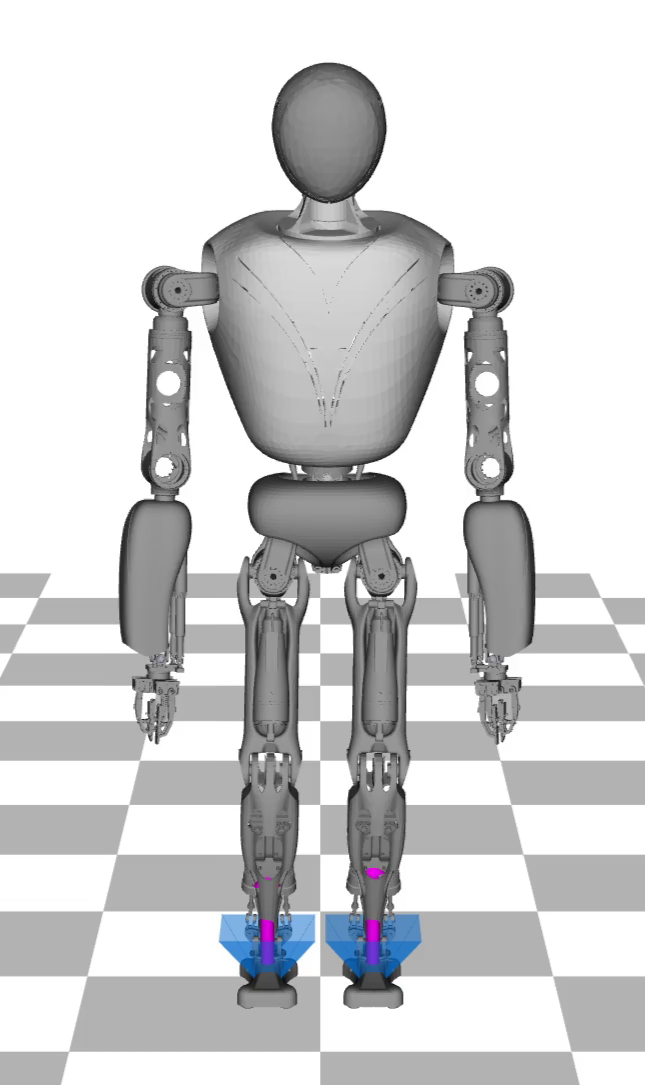
\includegraphics[width=.95\linewidth]{fig/walkStatic/snaps/1}
	\caption{}
\end{subfigure}%
\begin{subfigure}{.16\textwidth}
	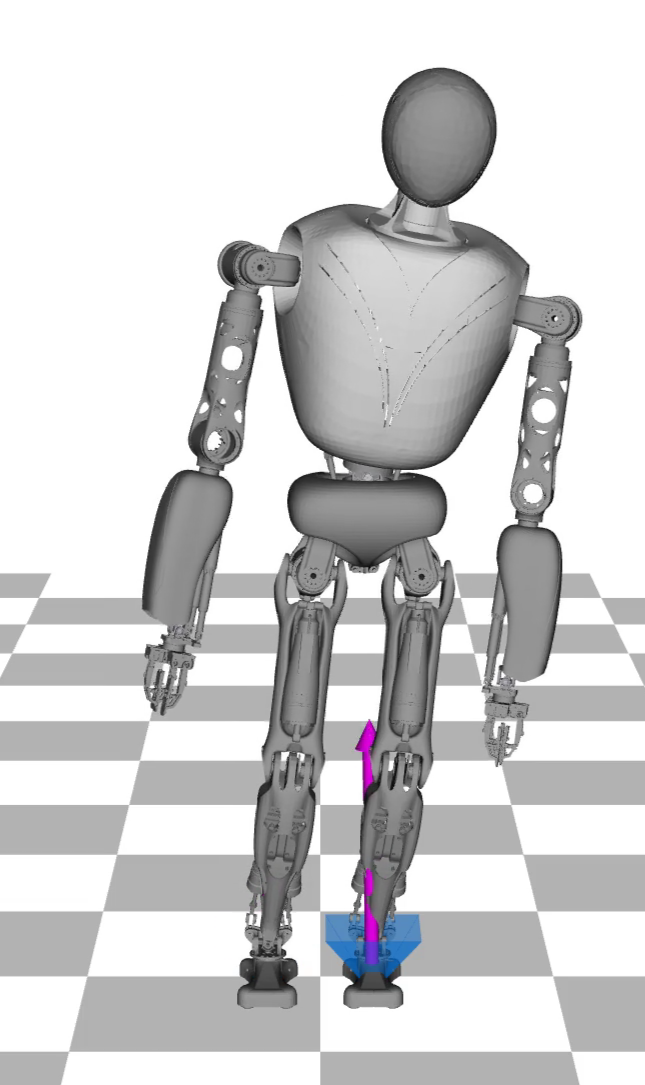
\includegraphics[width=.95\linewidth]{fig/walkStatic/snaps/2}
	\caption{}
\end{subfigure}%
\begin{subfigure}{.16\textwidth}
	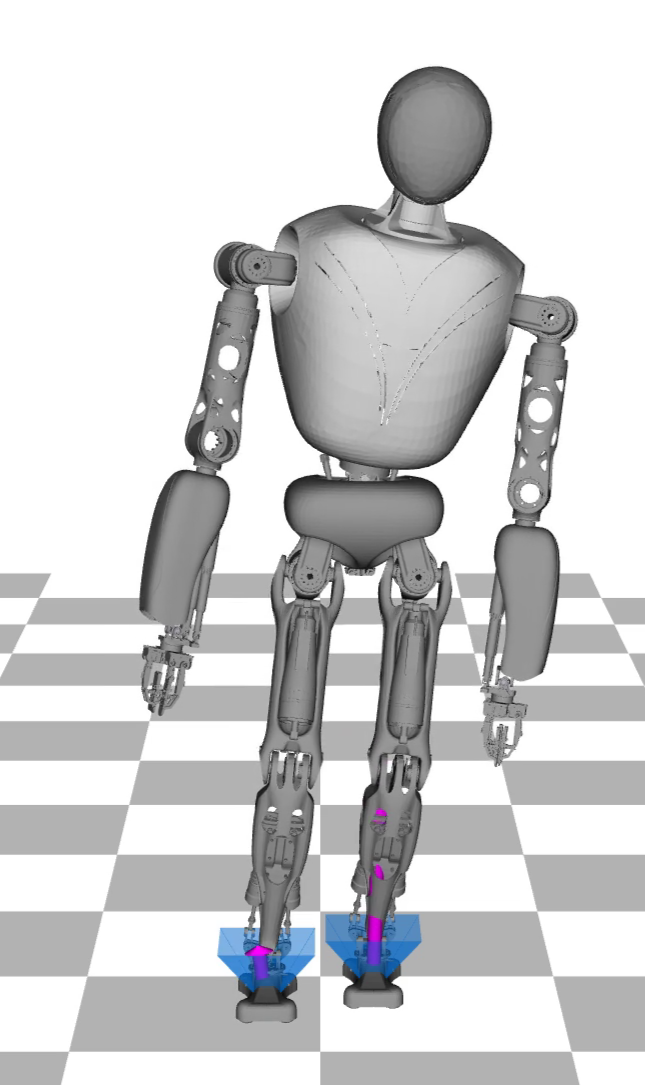
\includegraphics[width=.95\linewidth]{fig/walkStatic/snaps/4}
	\caption{}
\end{subfigure}%
\begin{subfigure}{.16\textwidth}
	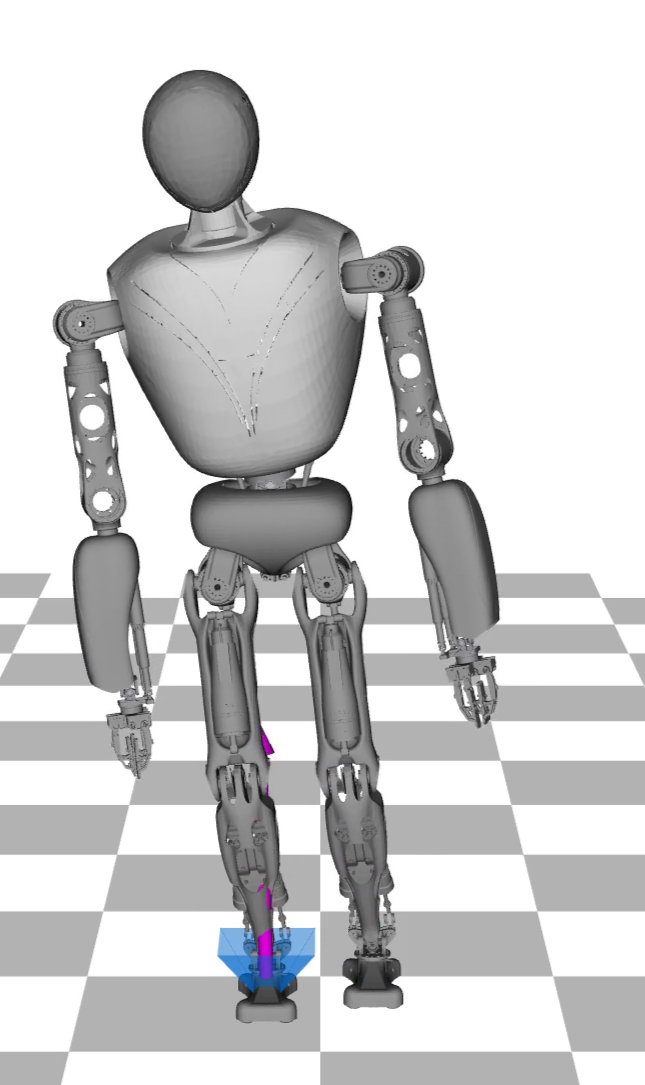
\includegraphics[width=.95\linewidth]{fig/walkStatic/snaps/6}
	\caption{}
\end{subfigure}%
\begin{subfigure}{.16\textwidth}
	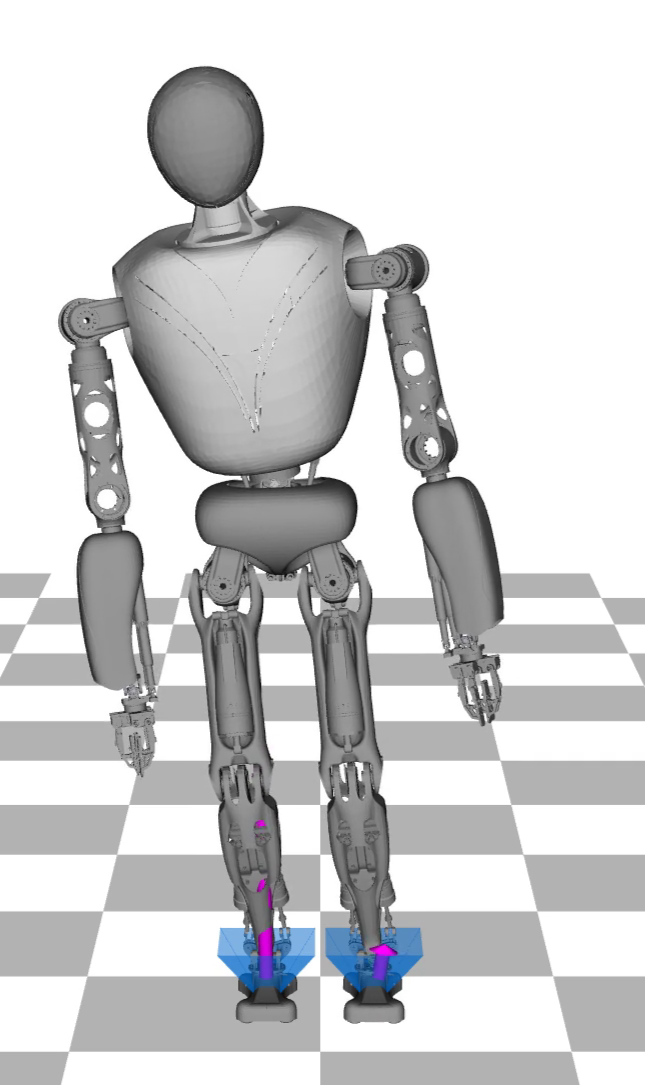
\includegraphics[width=.95\linewidth]{fig/walkStatic/snaps/8}
	\caption{}
\end{subfigure}%
\begin{subfigure}{.16\textwidth}
	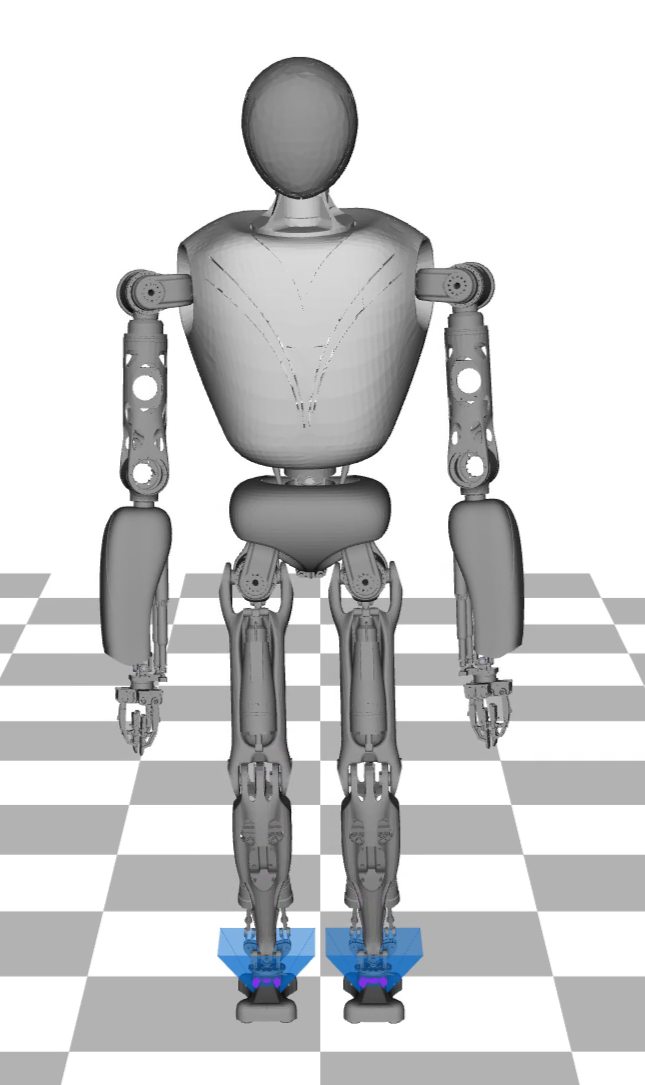
\includegraphics[width=.95\linewidth]{fig/walkStatic/snaps/9}
	\caption{}
\end{subfigure}
\caption[Static walking based on dedicated \gls{FCoM} shifting]{Static walking gait based on dedicated \gls{FCoM} motion, consisting of the locomotion phases (a) initial pose, (b) \gls{FCoM} shift above \gls{LF}, (c) right step, (d) \gls{FCoM} shift above \gls{RF}, (e) left step and (f) pose recovery. Significant lateral shifts of the \gls{FCoM} are required to establish the static stability. \href{https://github.com/julesser/ma-thesis-simulation-results/blob/master/HumanoidFixedArms/StaticWalking_NoCoPCost_ComHeightConstant/crocoddyl.mp4}{[Video]}}
\label{fig:walkStatic_Snaps}
\end{figure}

The results of the optimization problem \cref{eqn:optimizationProblem} are shown in \cref{fig:walkStatic_TaskSpace} and \cref{fig:walkStatic_JointState}.
\cref{fig:walkStatic_TaskSpace} presents the resulting base and end-effector trajectories. As becomes clear, the \gls{FCoM} tracking is sufficiently good and the \gls{CoM} height remains in a reasonable range of $\pm$ 1 cm. Equally, the desired foot trajectory is tracked with adequate accuracy. Also, the foot velocities are reasonable with a maximum velocity of 0.1 m/s at the impact. The pursued step height is not reached exactly but is about one centimeter less. This effect can be explained by the immediately reverse direction at the vertex of the piecewise-linear trajectory, which is smoothened by the solver.

\cref{fig:walkStatic_JointState} shows the resulting joint trajectories for the torso, \gls{LF} and \gls{RF}. Both the joint position limits and the maximum permissible joint speeds remain far below the limits due to the slow nature of the motion. Interestingly, the pursued \gls{FCoM} shifting turns out to be realized mostly based on a shift in the body roll activation rather than on a shift in the hips. Furthermore, it becomes evident that the posture regularization is effective since all joints end closely to the initial position.

\begin{figure}[h!]
\centering	
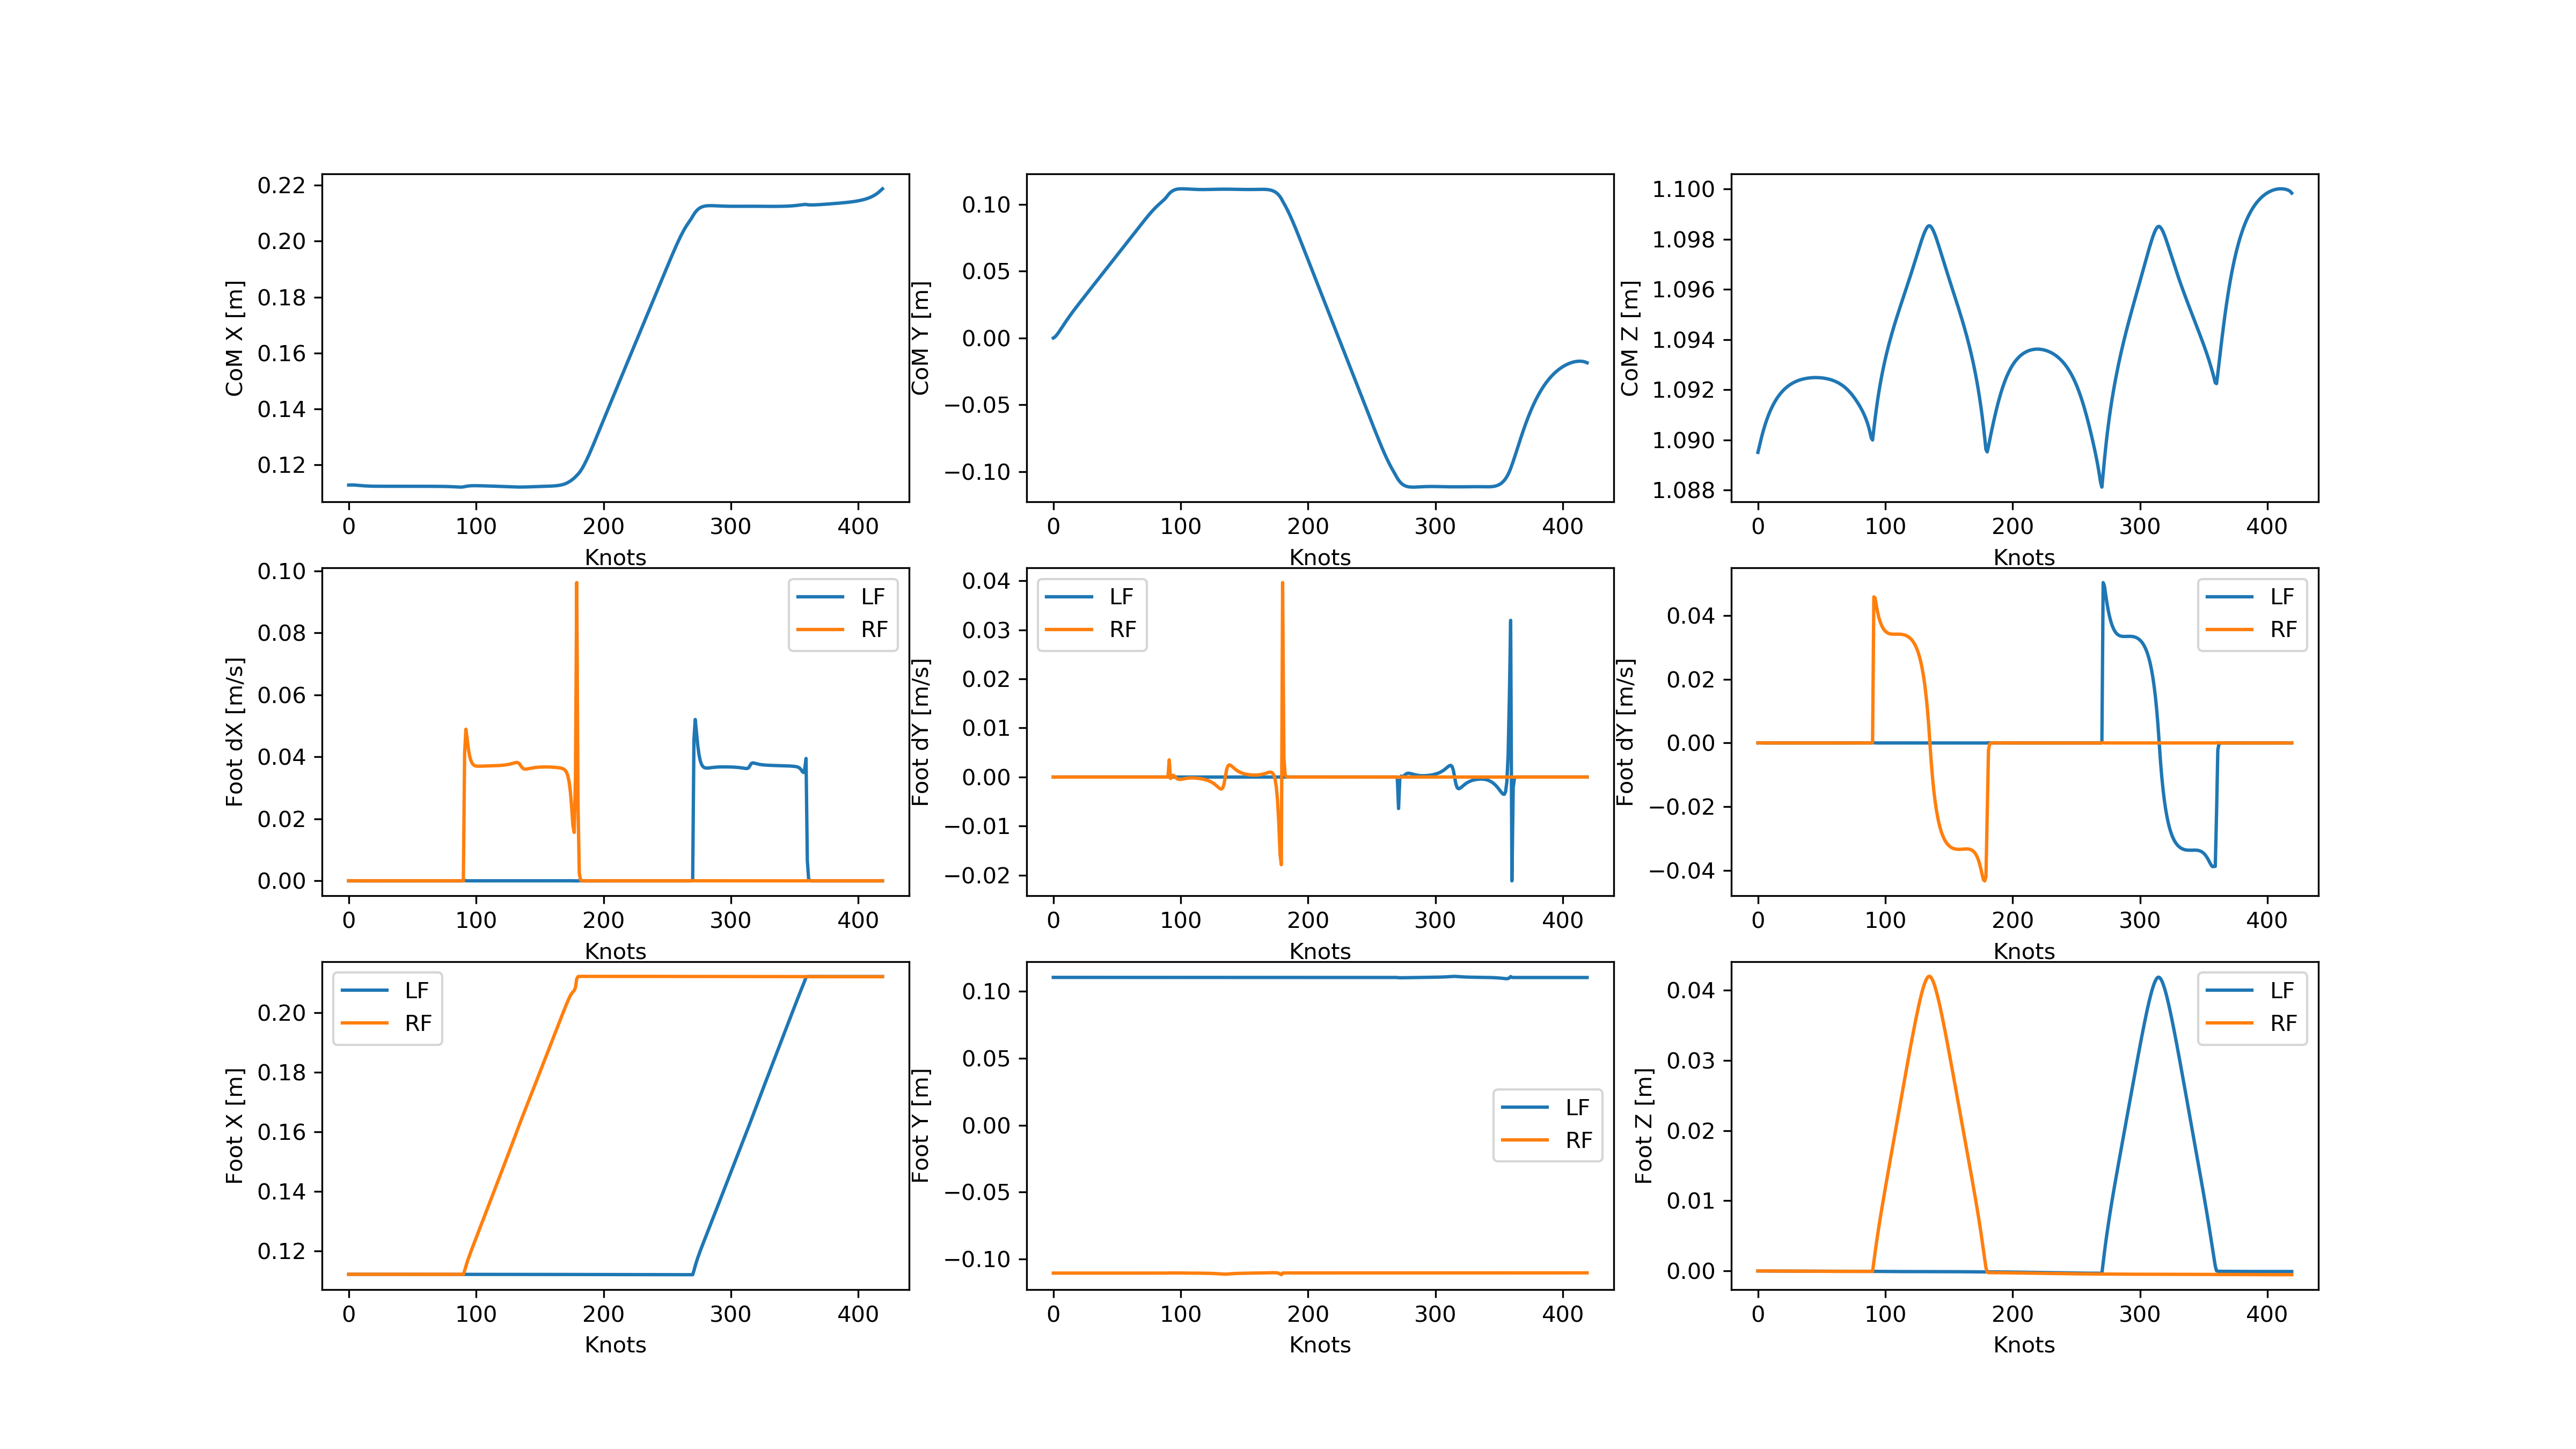
\includegraphics[width=1\textwidth]{fig/walkStatic/TaskSpace}
\caption[Static walking gait solution in task space]{Static walking gait solution in task space. Both the \gls{FCoM} task and the swing foot task are satisfied with acceptable accuracy.}
\label{fig:walkStatic_TaskSpace}
\end{figure} 

\begin{figure}[h!]
\centering	
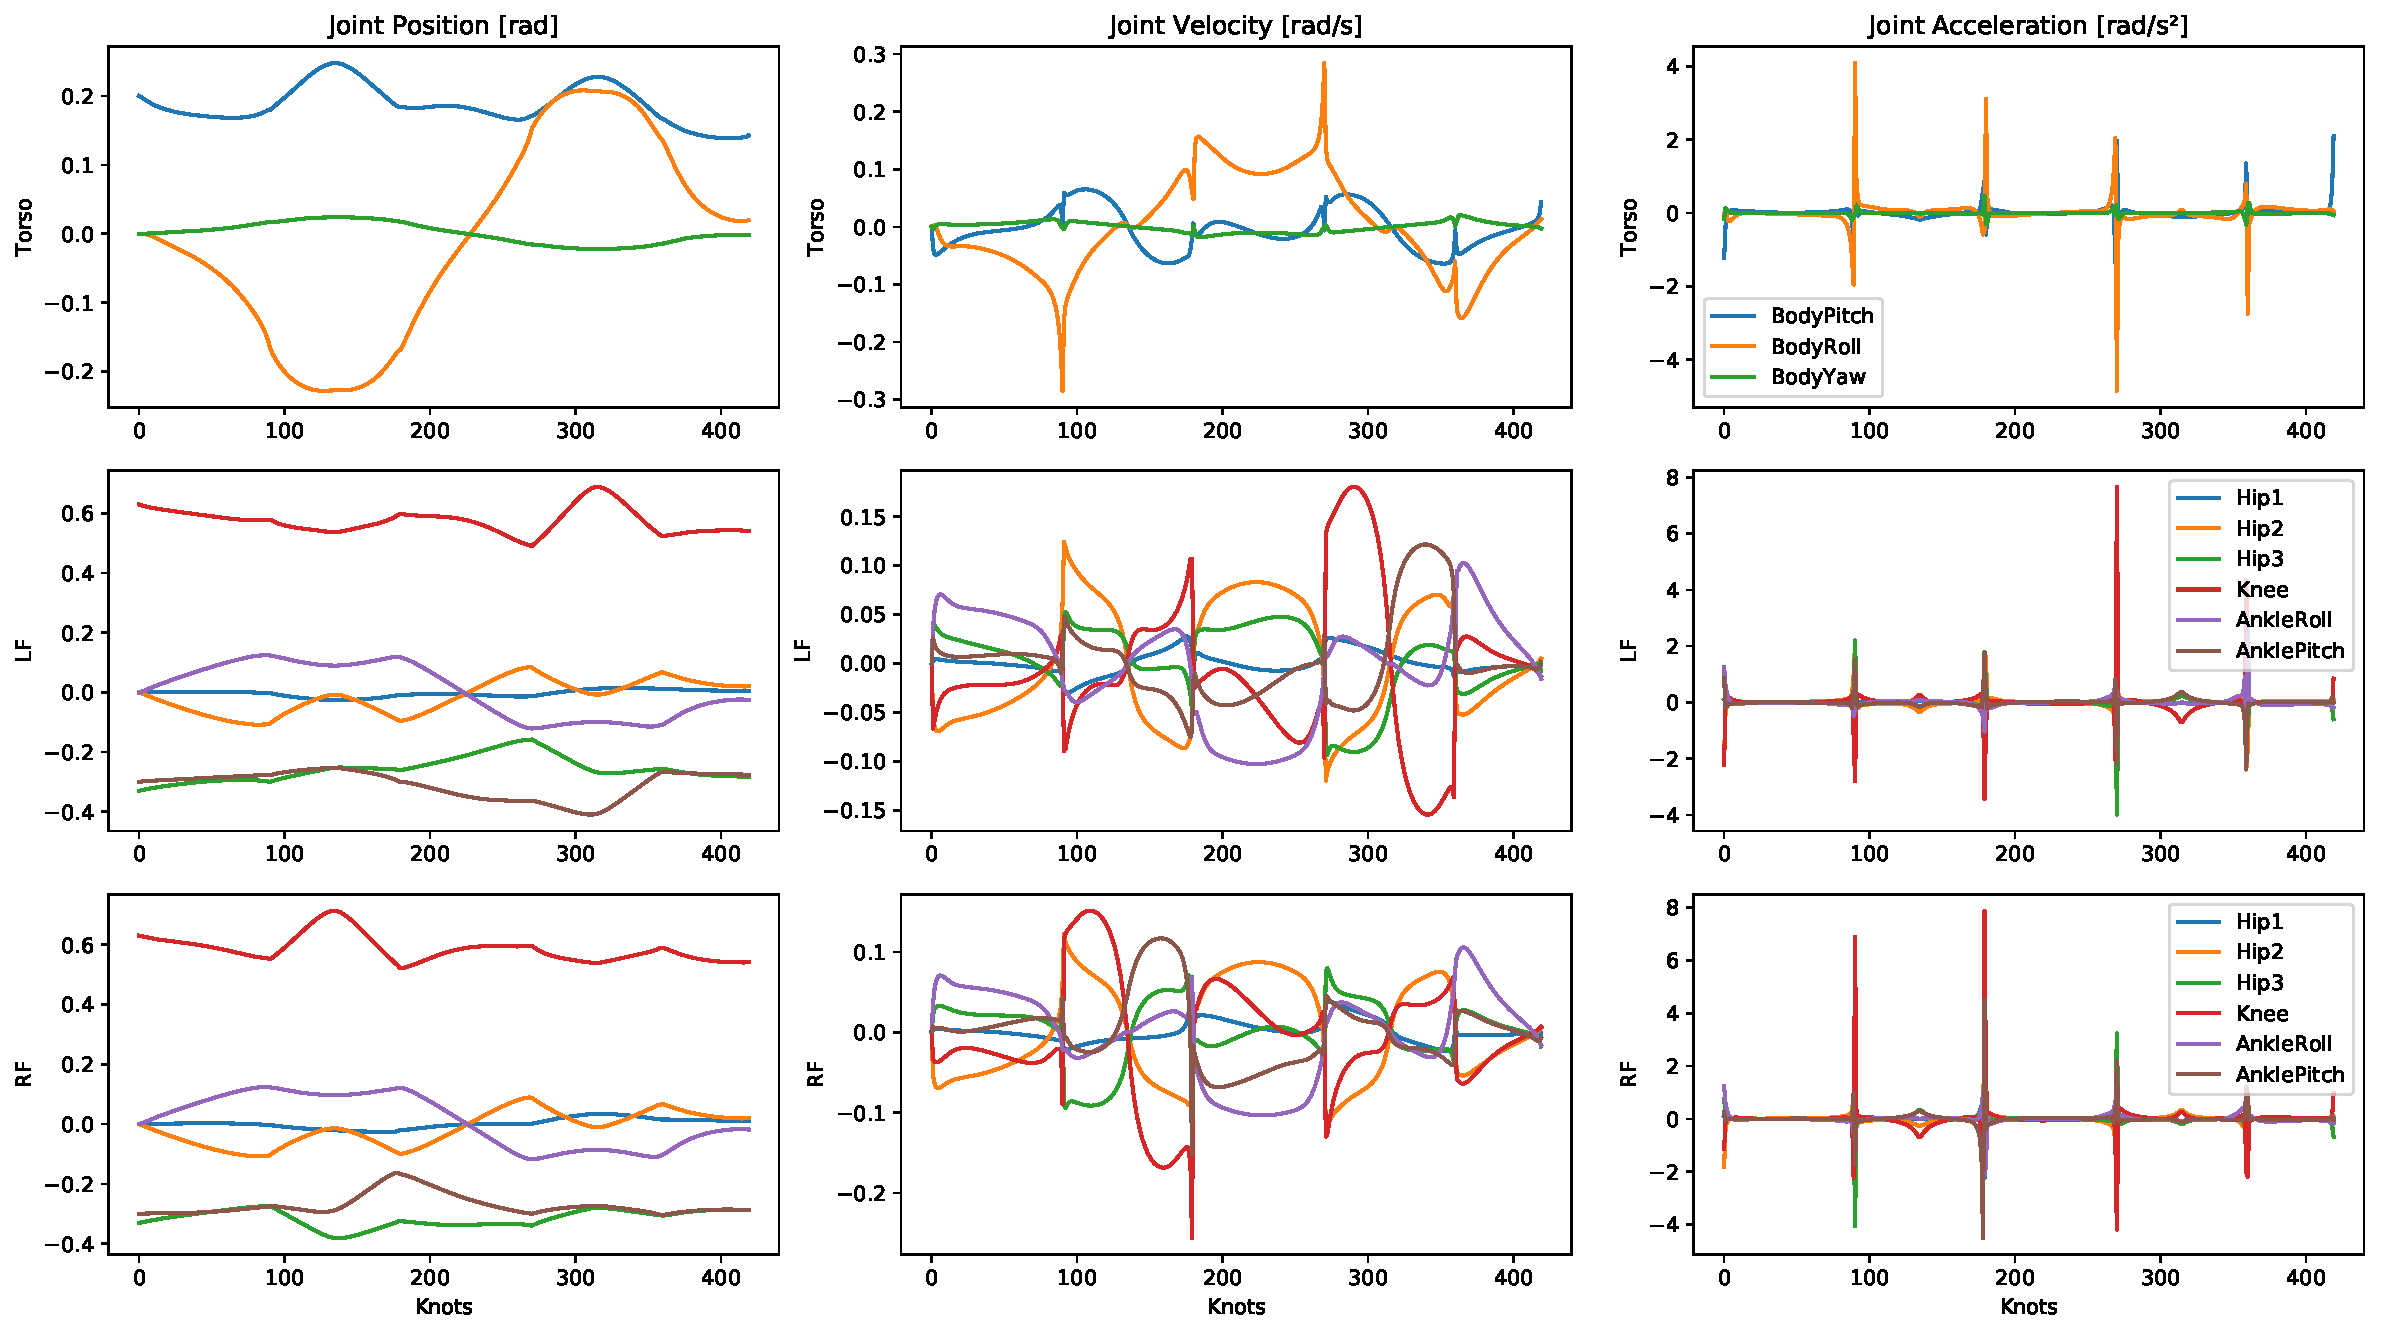
\includegraphics[width=1\textwidth]{fig/walkStatic/JointState}
\caption[Static walking gait solution of the joint states]{Static walking gait solution of the joint states. Due to the slow nature of the motion, joint limits are far from being reached and velocity discontinuities remain within reasonable ranges.}
\label{fig:walkStatic_JointState}
\end{figure} 

\subsection{Dynamic Walking}
The analysis of a dynamic walking gait is concerned about generating efficient motions with higher velocities. This part forms the basis of the stability evaluation in the next section.

Focus of investigation is a dynamic walking motion. Compared to the previously studied static walking gait these motions are characterized by higher velocities and dynamic forces exceeding the static ones. These characteristics imply that dynamic stability criteria become necessary. To this end, we apply the proposed approach of contact stability constrained DDP described in \cref{c3}. Consequently, the \gls{CoP} of each foot is constrained instead of following a reference \gls{CoM} trajectory. By this, the solver is enabled to find an optimal, dynamic \gls{CoM} shifting along with the requested contact stability constraints. 

\cref{tab:walkDynamic} compactly summarizes the gait characteristics and applied optimization constraints. The optimization problem is composed of a total of five locomotion phases visualized in \cref{fig:walkDynamic_Snaps}. From (a) an initial pose in \gls{DS}, (b,c) perform a right step, (d,e) perform a left step and (f) recover to the initial pose. In accordance with biomechanical findings \cite{kuo2001simple}, we choose a desired step length of 40 \nolinebreak cm with 1.5 s per step and deliberately define a stance to swing ratio of one to three.

\begin{table}[t]
\centering
\caption[Dynamic walking gait characteristics and optimization constraints]{Dynamic walking gait characteristics and optimization constraints for a stance to swing ratio of one to three.}
\begin{tabular}{|ll|ll|}
\hline
\multicolumn{2}{|l|}{\textbf{Gait Characteristics}} & \multicolumn{2}{l|}{\textbf{Optimization Constraints}} \\ \hline
Step length:& 40 cm 	& Tasks: 			& $\Phi_{\text{foot}}$\\ \hline
Step height:& 5 cm 	& Stability: 		&$\Phi_{\text{CoP}}$, $\Phi_{\text{friction}}$ \\ \hline
Time:& 1.5 s/step	& Limits: 			& $\Phi_{\text{joint}}$, torques \\ \hline
Step size:& 0.03 s	& Regularization: 	& $\Phi_{\text{posture}}$, $\Phi_{\text{torque}}$\\ \hline
\end{tabular}
\label{tab:walkDynamic}
\end{table} 

\begin{figure}
\begin{subfigure}{.16\textwidth}
	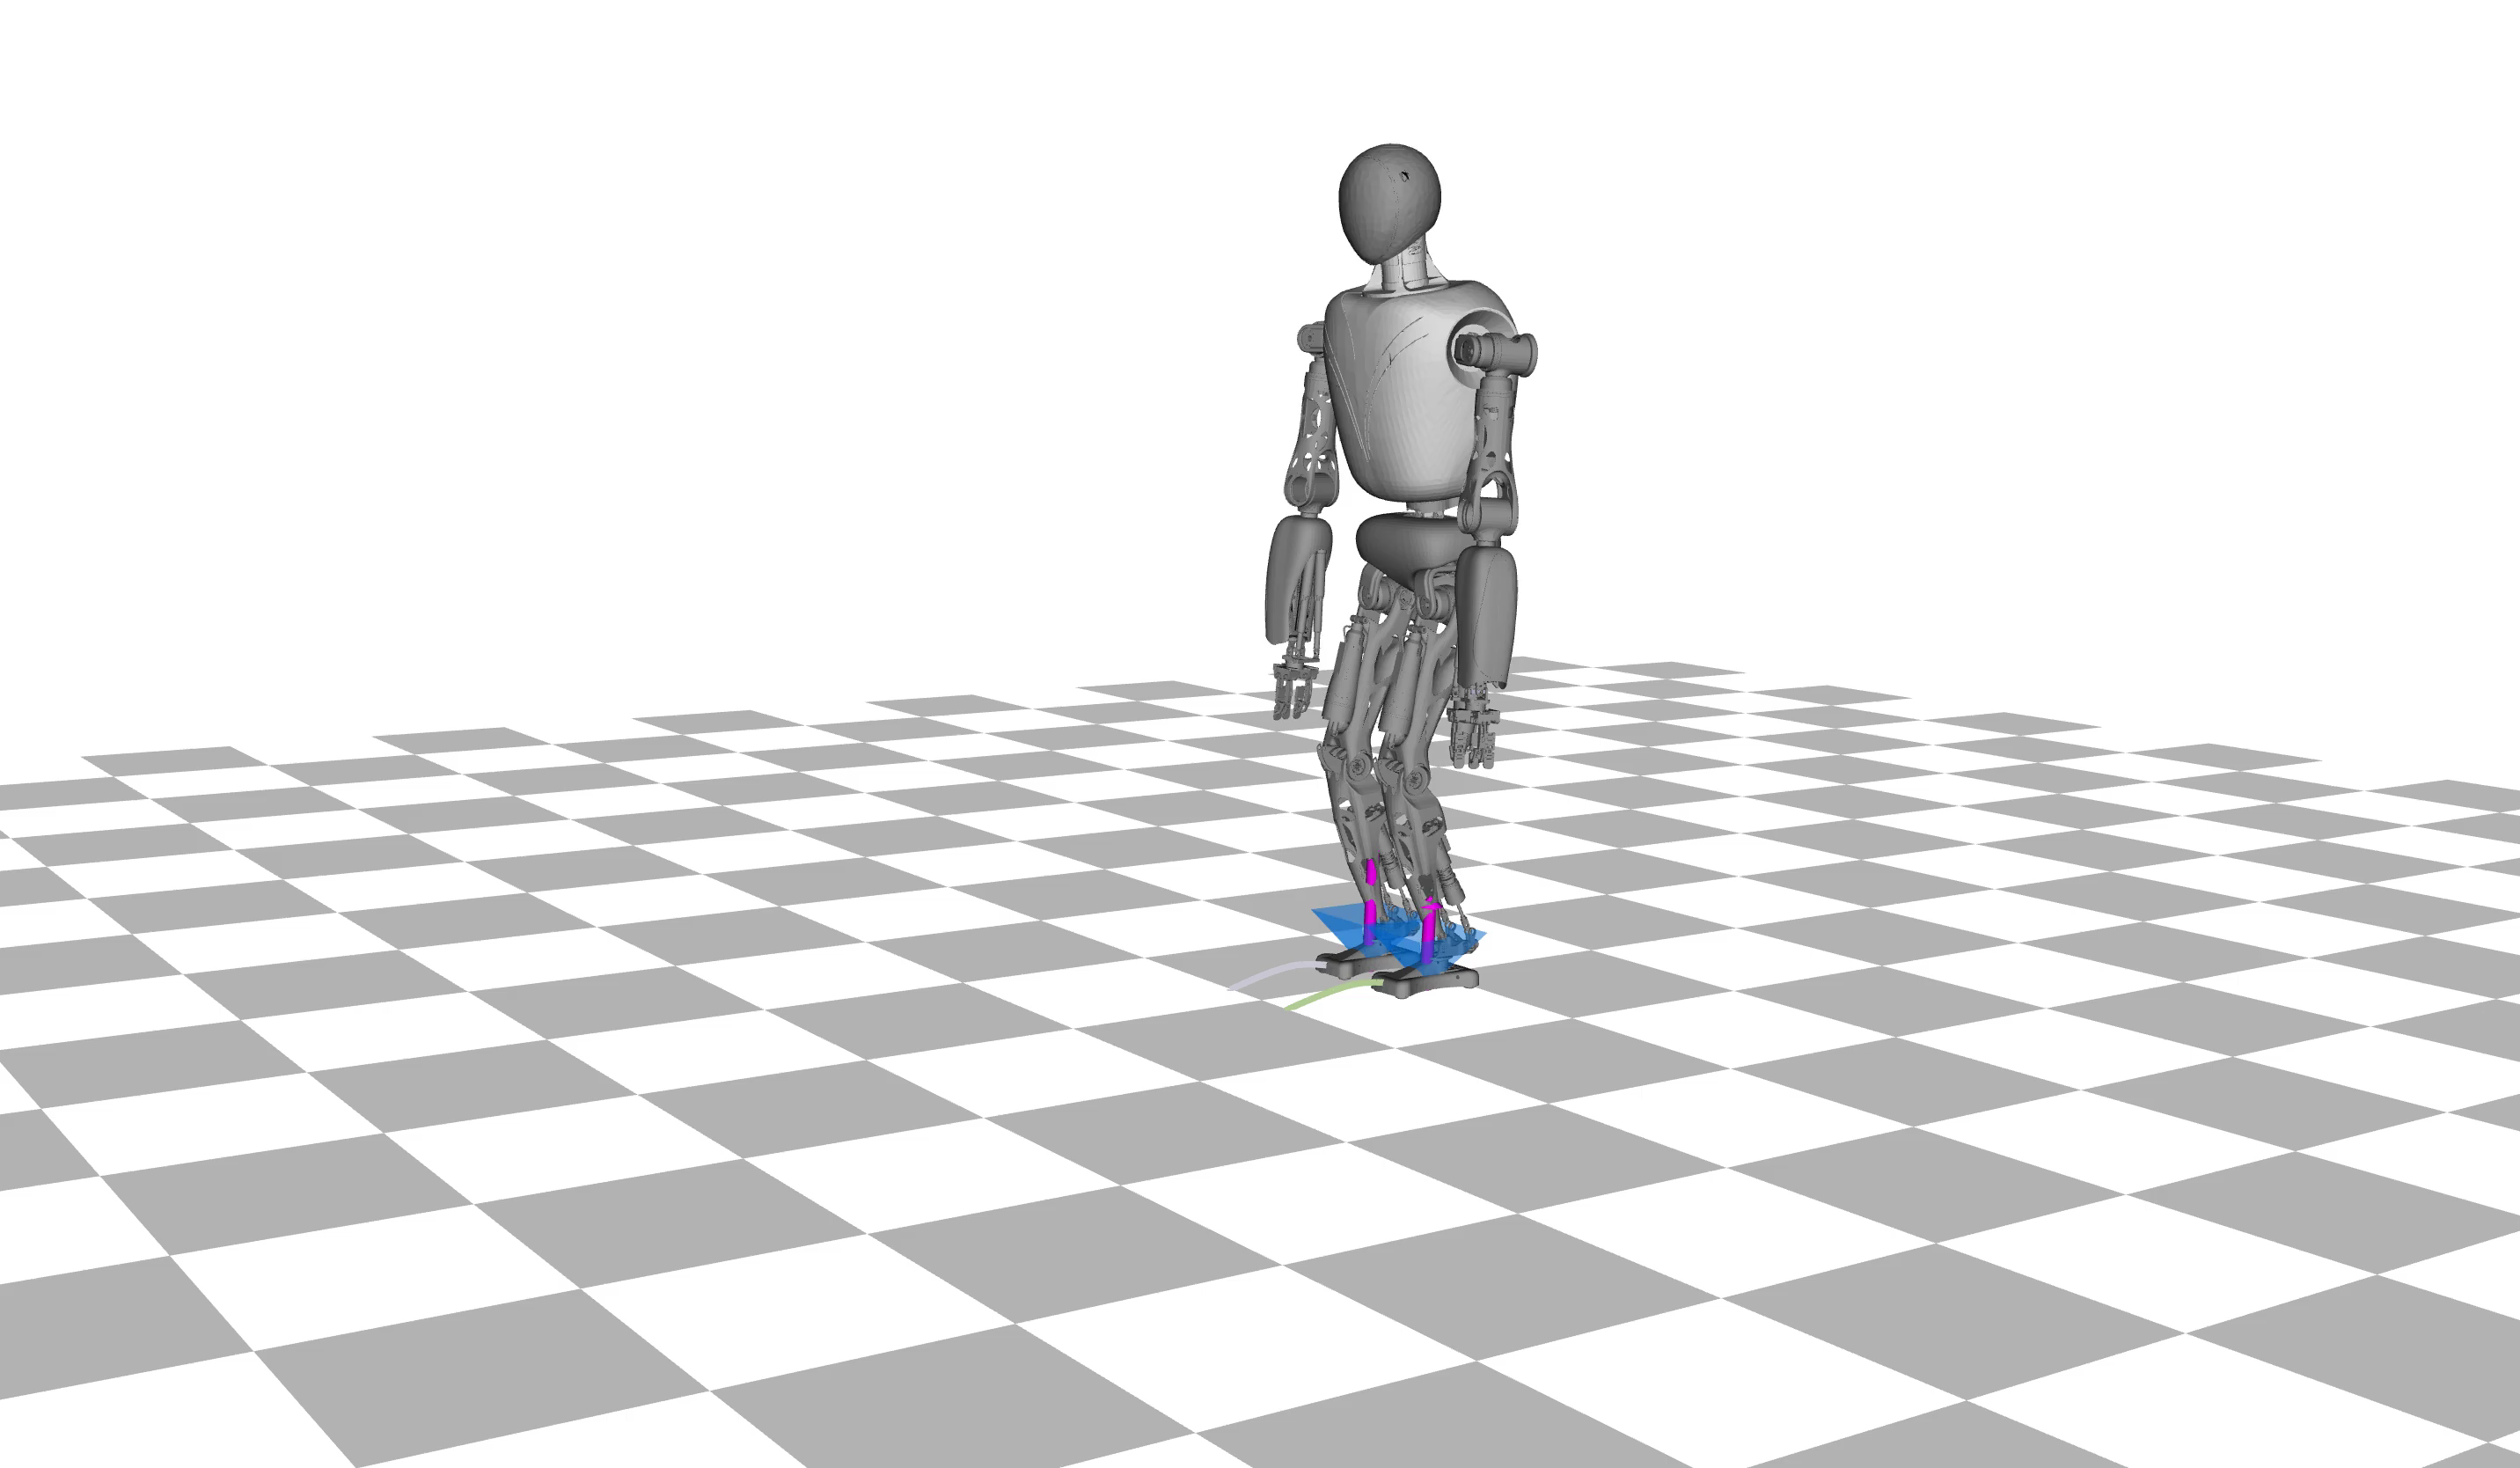
\includegraphics[width=.95\linewidth]{fig/walkDynamic/snaps/1}
	\caption{}
\end{subfigure}%
\begin{subfigure}{.16\textwidth}
	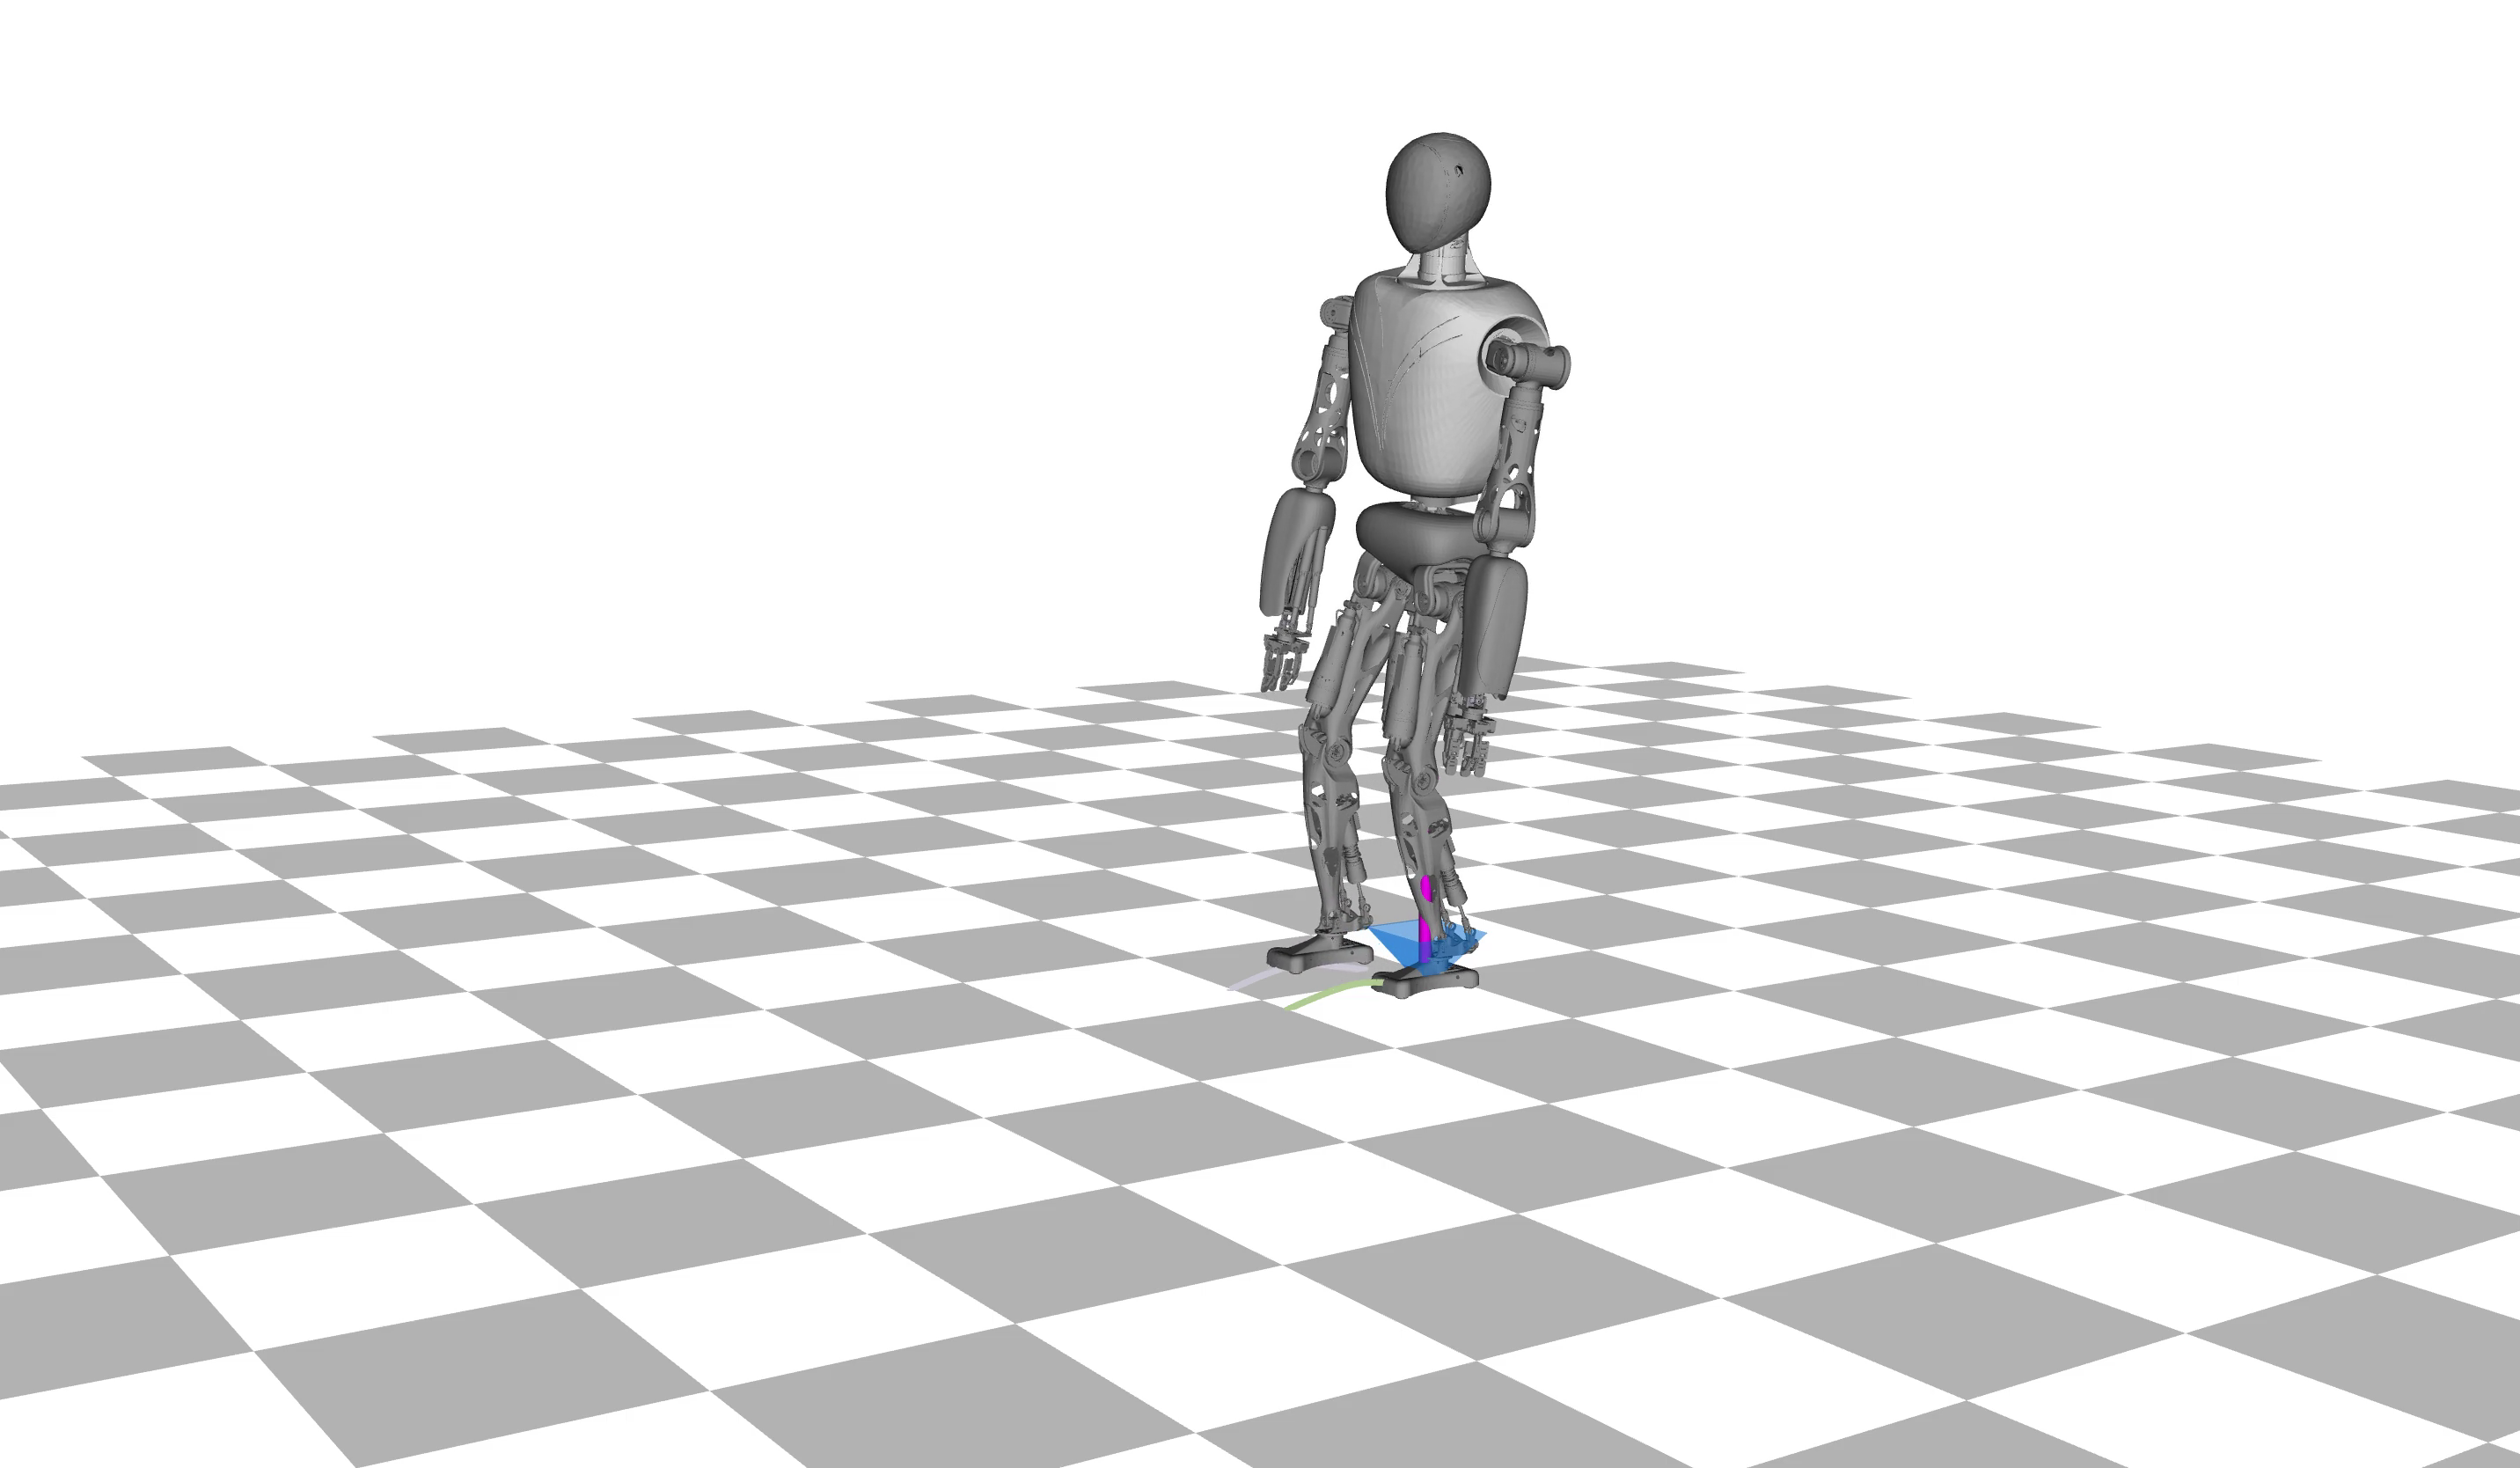
\includegraphics[width=.95\linewidth]{fig/walkDynamic/snaps/3}
	\caption{}
\end{subfigure}%
\begin{subfigure}{.16\textwidth}
	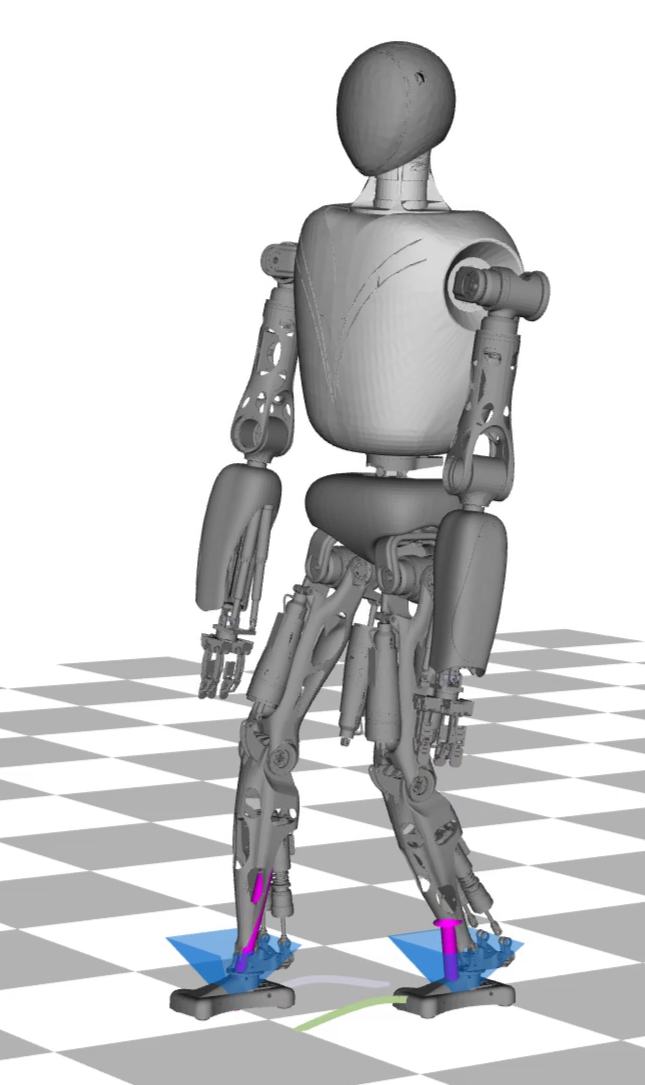
\includegraphics[width=.95\linewidth]{fig/walkDynamic/snaps/4}
	\caption{}
\end{subfigure}%
\begin{subfigure}{.16\textwidth}
	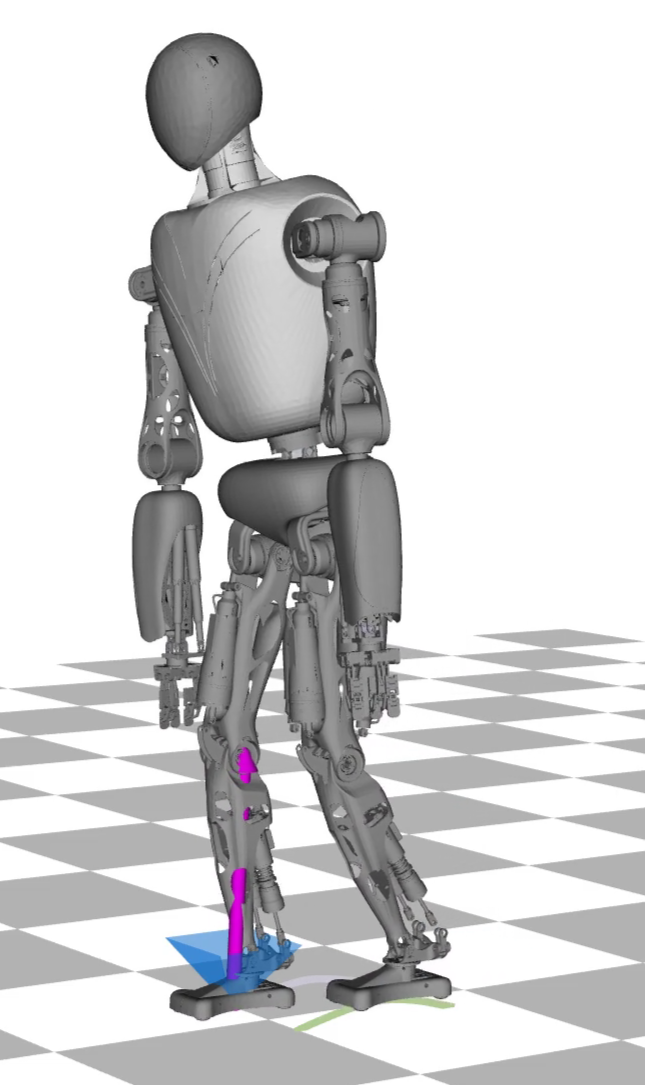
\includegraphics[width=.95\linewidth]{fig/walkDynamic/snaps/6}
	\caption{}
\end{subfigure}%
\begin{subfigure}{.16\textwidth}
	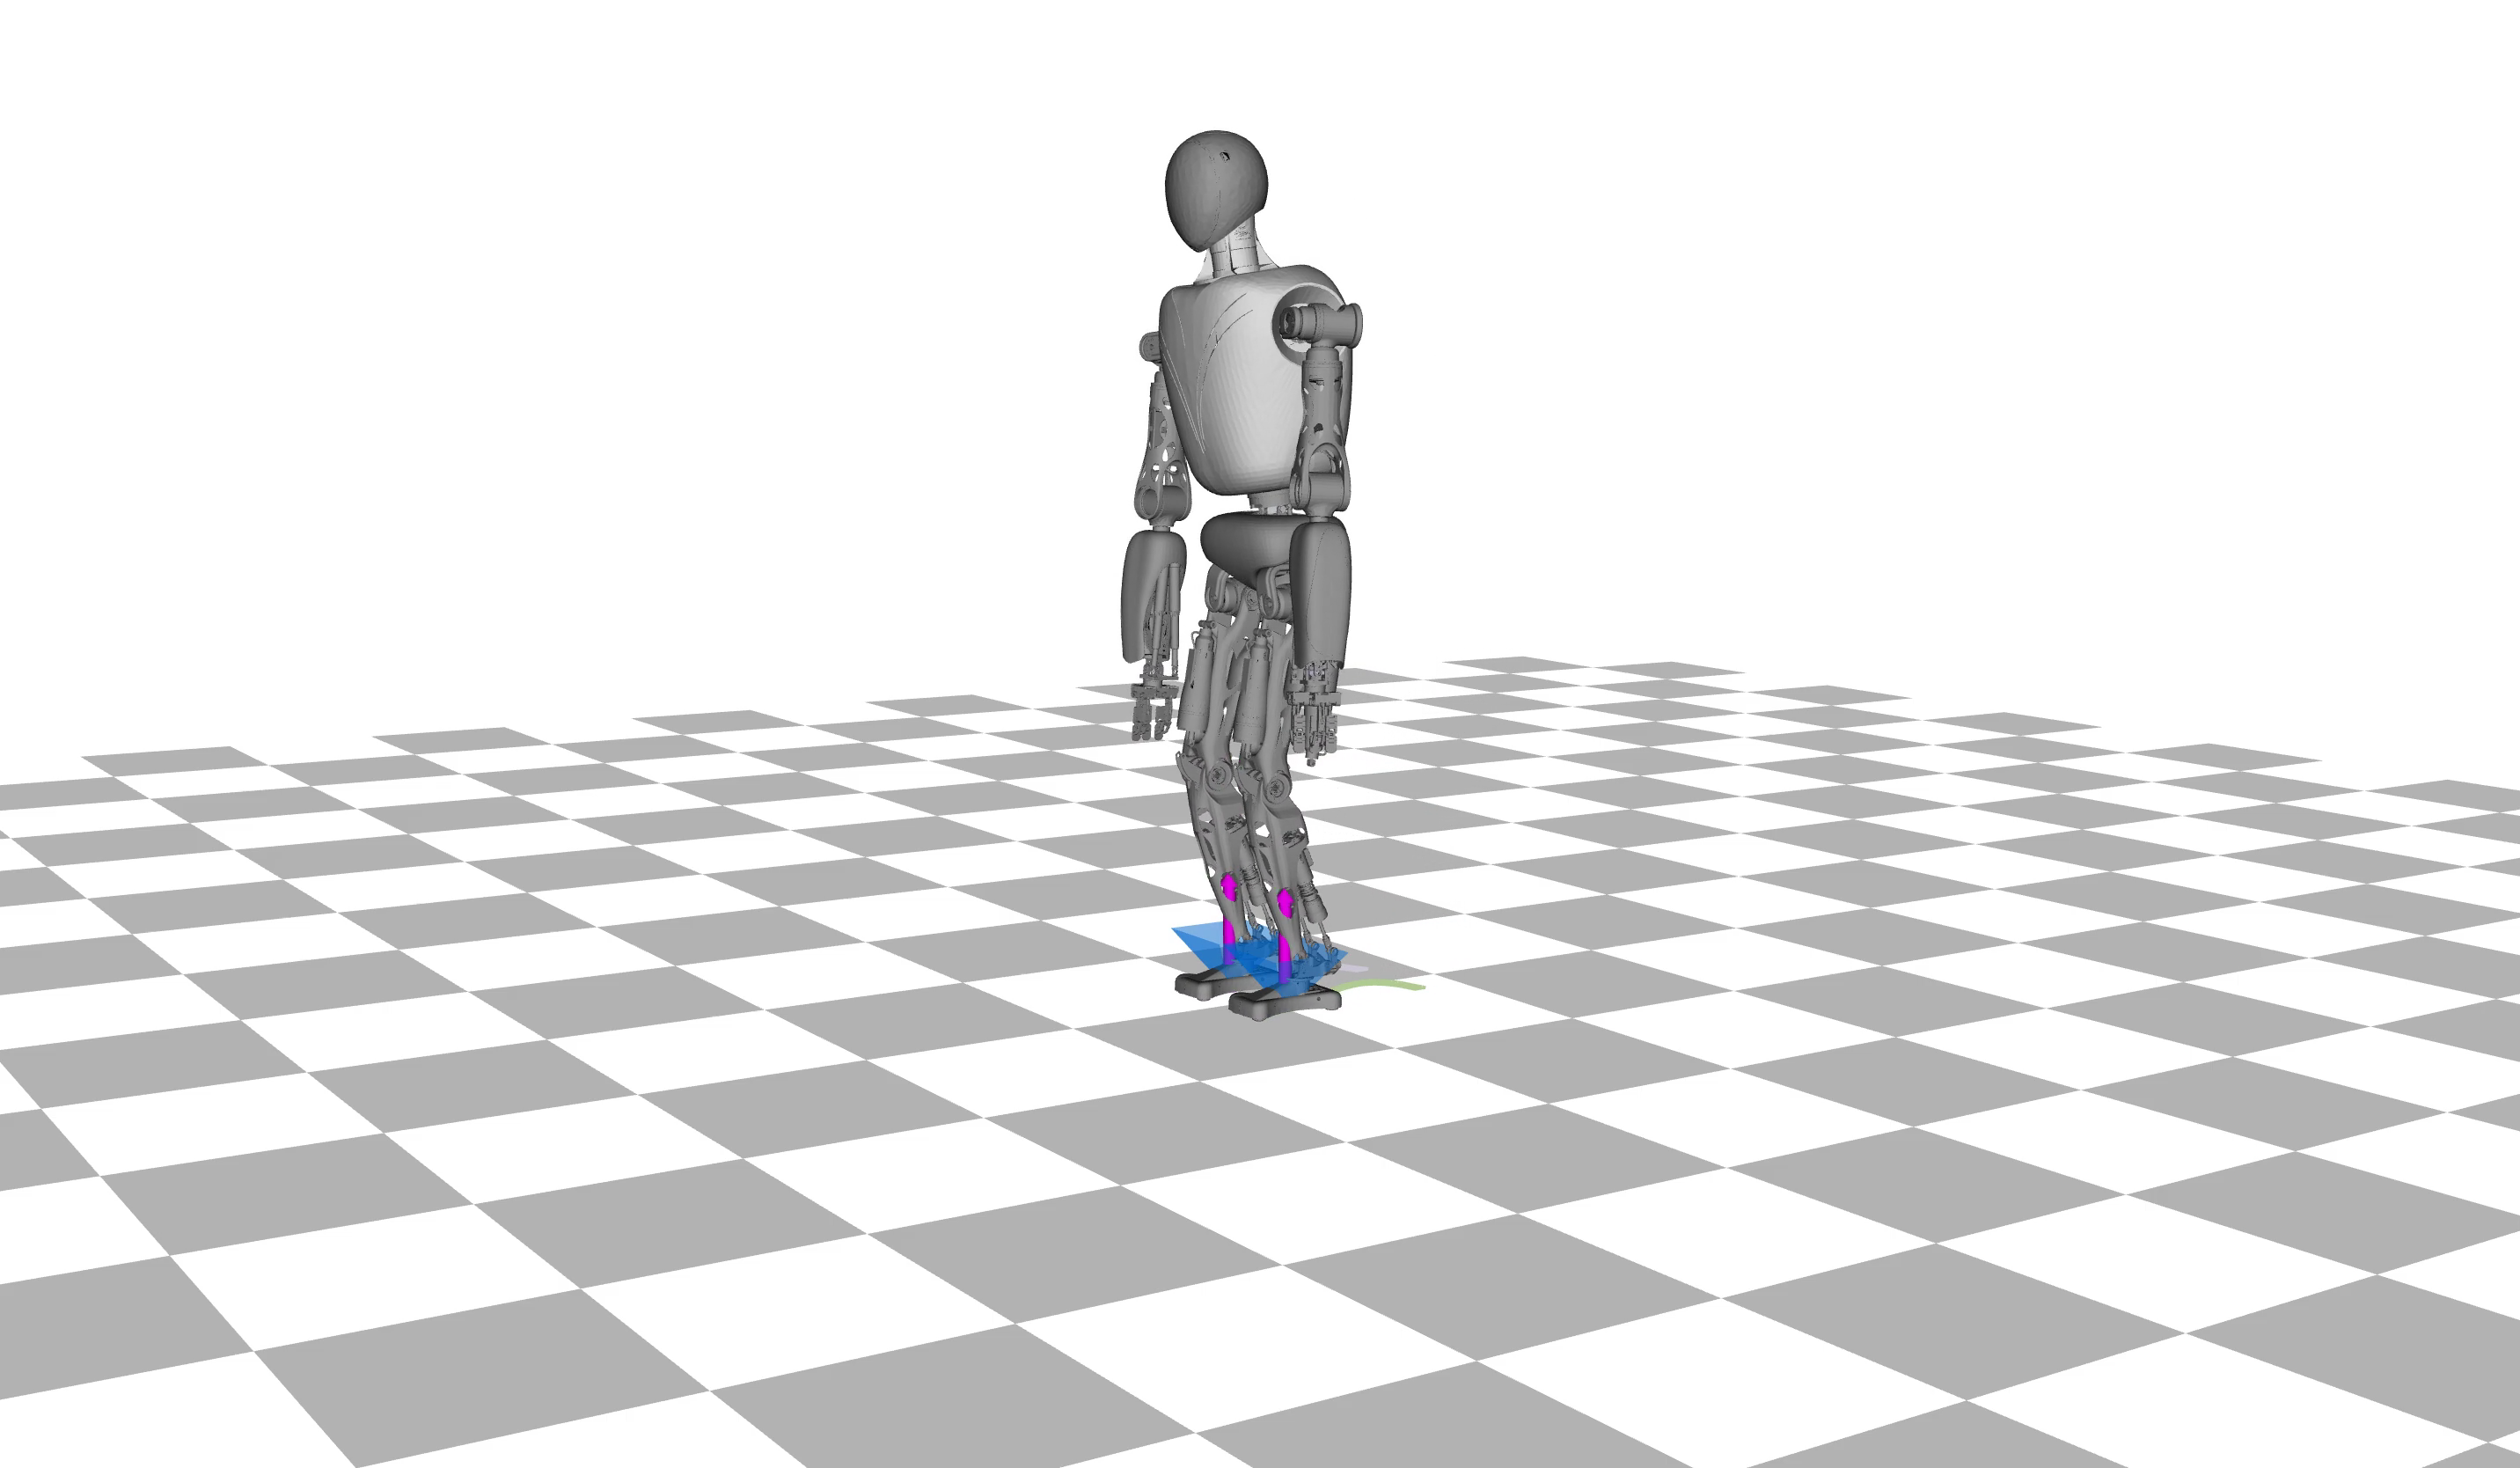
\includegraphics[width=.95\linewidth]{fig/walkDynamic/snaps/7}
	\caption{}
\end{subfigure}%
\begin{subfigure}{.16\textwidth}
	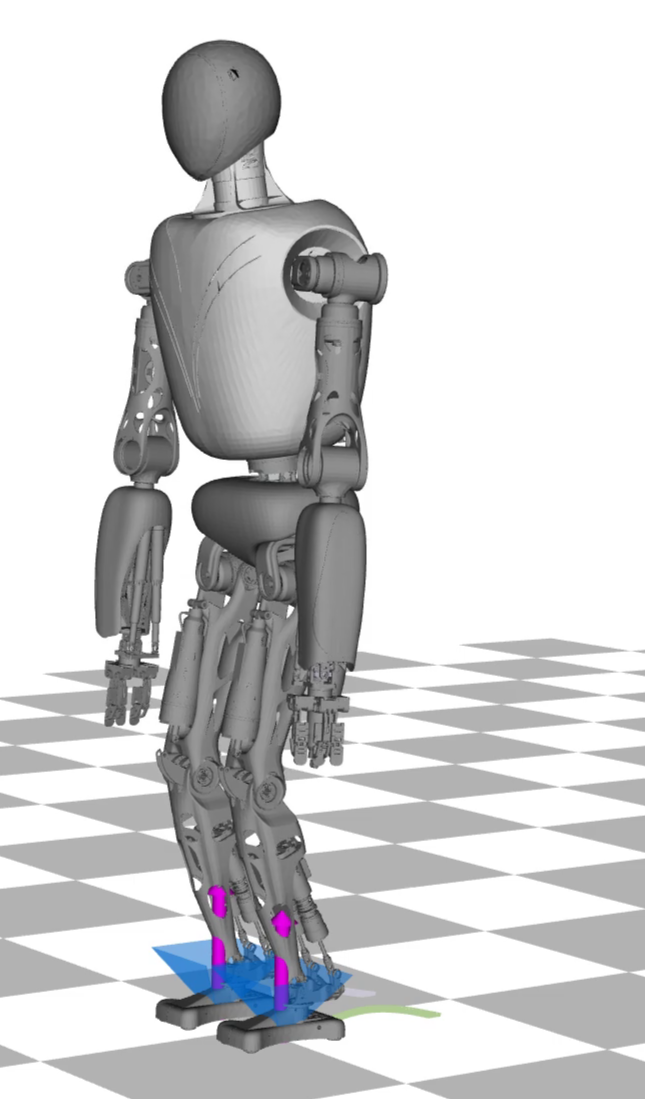
\includegraphics[width=.95\linewidth]{fig/walkDynamic/snaps/8}
	\caption{}
\end{subfigure}
\caption[Dynamic walking based on the contact stability constrained \gls{DDP}]{Dynamic walking gait based on the contact stability constrained \gls{DDP} approach, consisting of the locomotion phases (a) initial pose, (b,c) right step, (d,e) left step and (f) pose recovery. A natural \gls{CoM} shifting emerges resulting from the inequality constraints for the \gls{CoP} of each foot. \href{https://github.com/julesser/ma-thesis-simulation-results/blob/master/DynamicWalking_LargeSteps_CoP100_ArmsFreed/crocoddyl.mp4}{[Video]}}
\label{fig:walkDynamic_Snaps}
\end{figure}

As becomes clear from \cref{fig:walkDynamic_TaskSpace}, a natural \gls{CoM} shifting to the sides emerges resulting from the inequality constraints for the \gls{CoP}, which is about half of the amount as for the static walking case. Although the \gls{CoM} height is not explicitly constrained, it stays in a reasonable range of about $+$3 cm, which may be caused from the final posture regularization. The end-effector velocities in z-direction are about twice as high as for the case of static walking, which is explained by the higher walking speed. 
\cref{fig:walkDynamic_JointState} shows the resulting joint states for the dynamic walking gait. The velocity and acceleration contain higher peaks and the joint deflections are stronger, which is reasonable due to the higher walking speed.       

\begin{figure}[h!]
\centering	
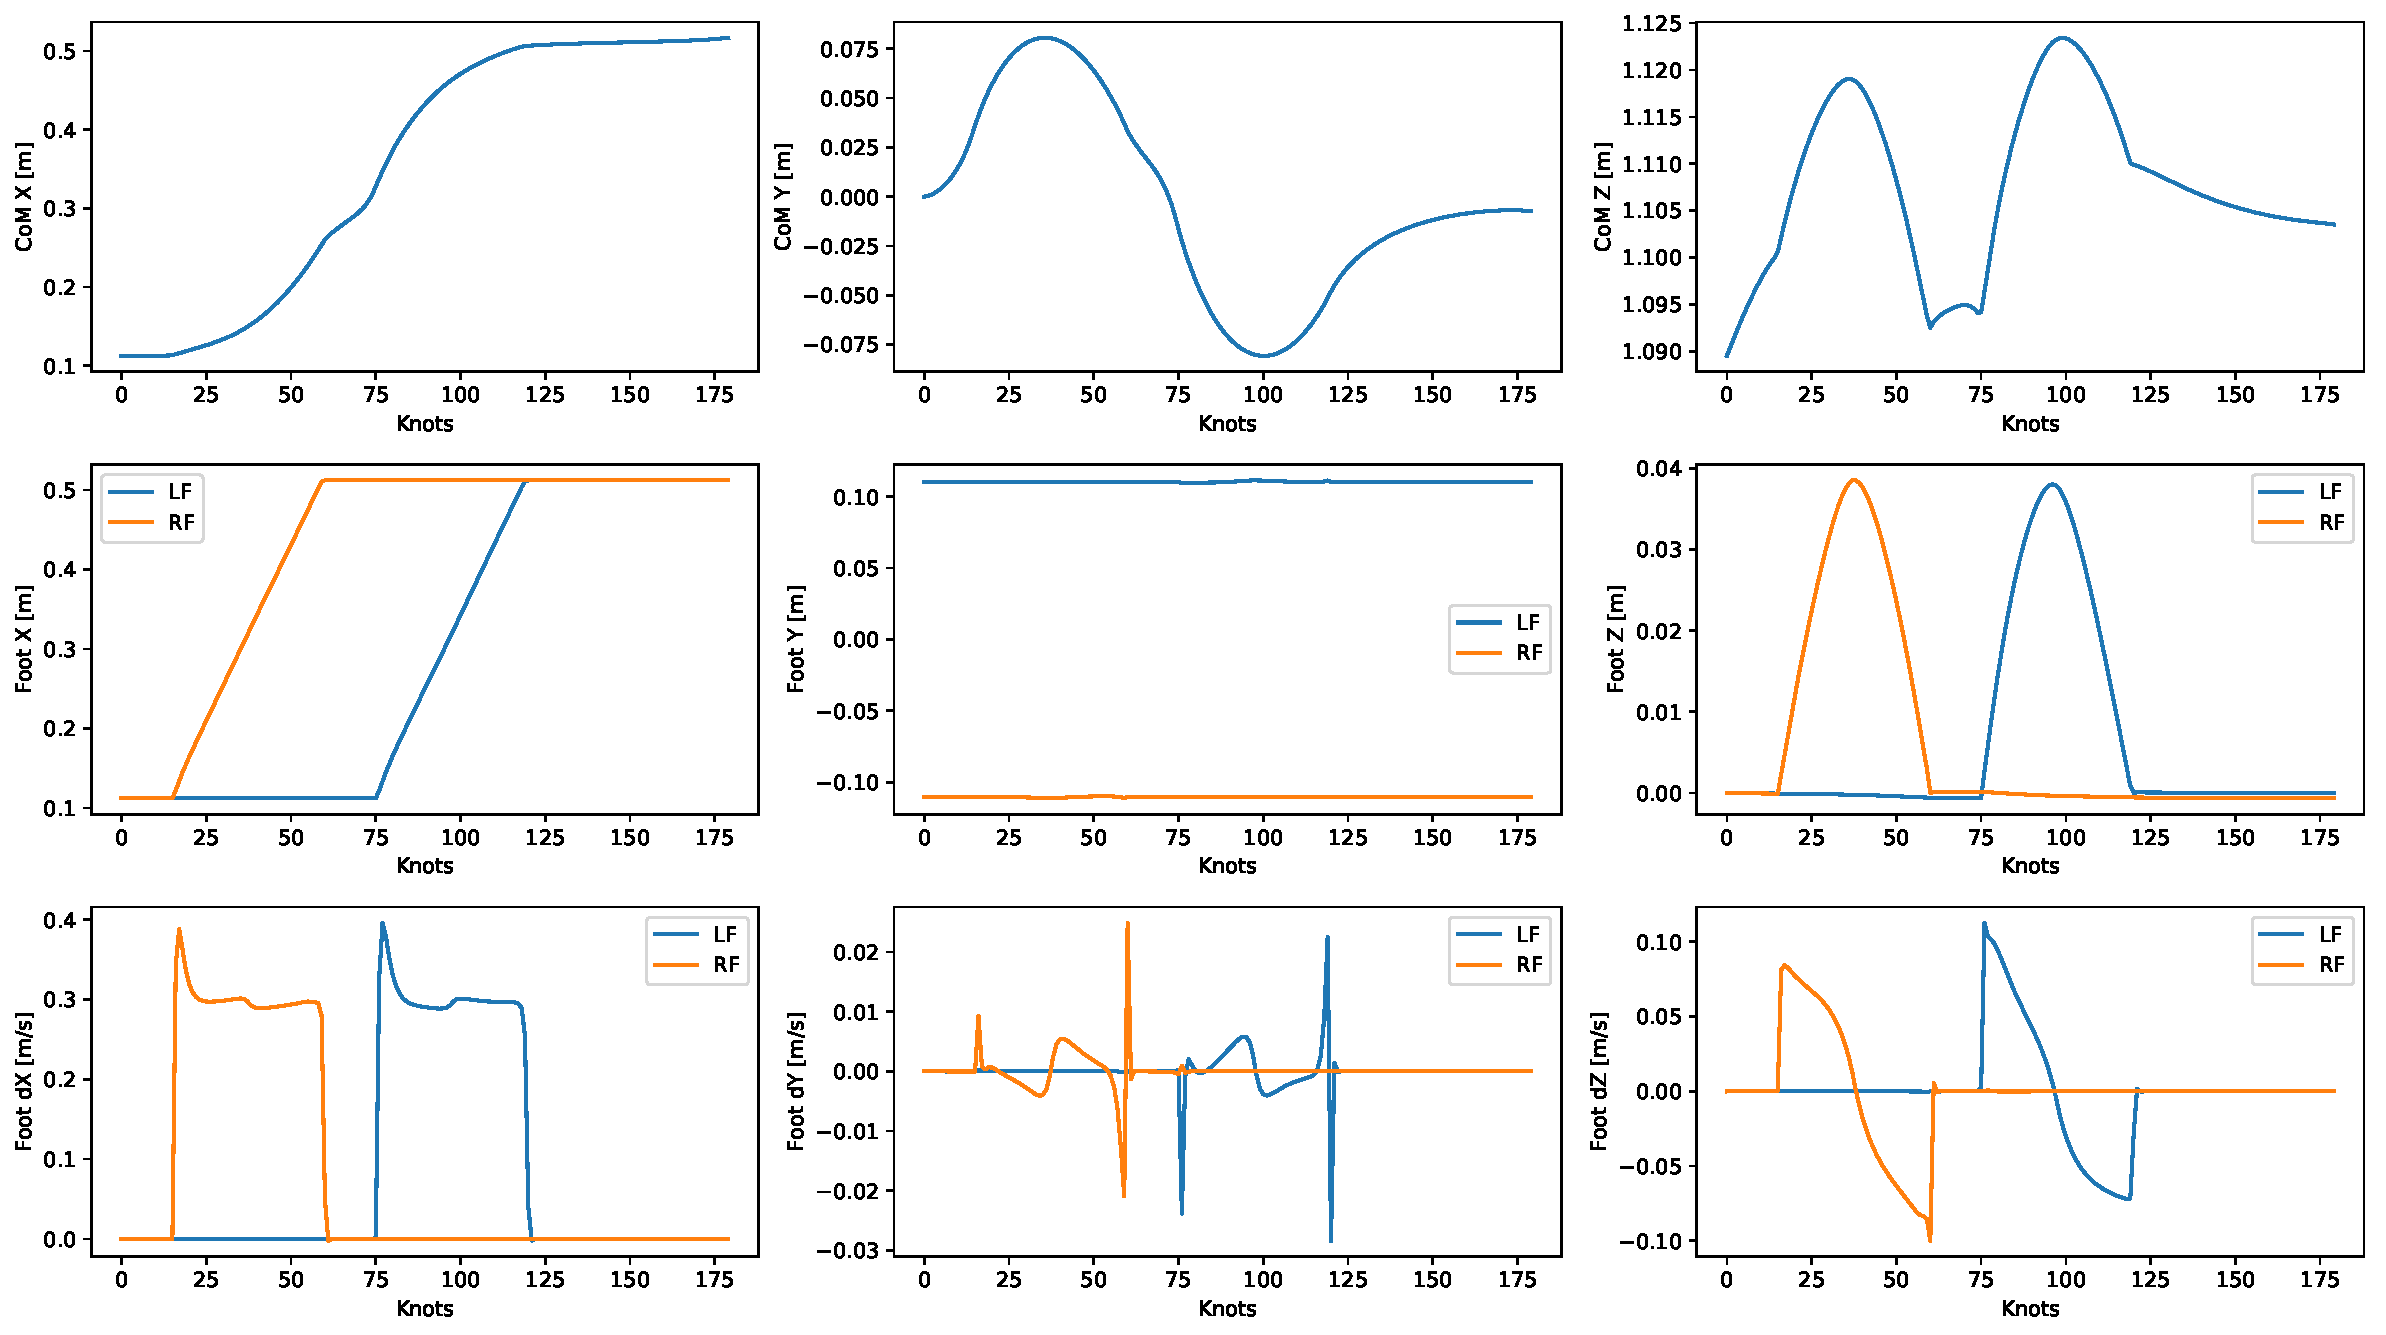
\includegraphics[width=.9\textwidth]{fig/walkDynamic/TaskSpace}
\caption[Dynamic walking gait solution in task space]{Dynamic walking gait solution in task space. It becomes evident that a natural \gls{CoM} shifting in y-direction emerges resulting from the inequality constraints for the \gls{CoP} of each foot.}
\label{fig:walkDynamic_TaskSpace}
\end{figure} 

\begin{figure}[h!]
\centering	
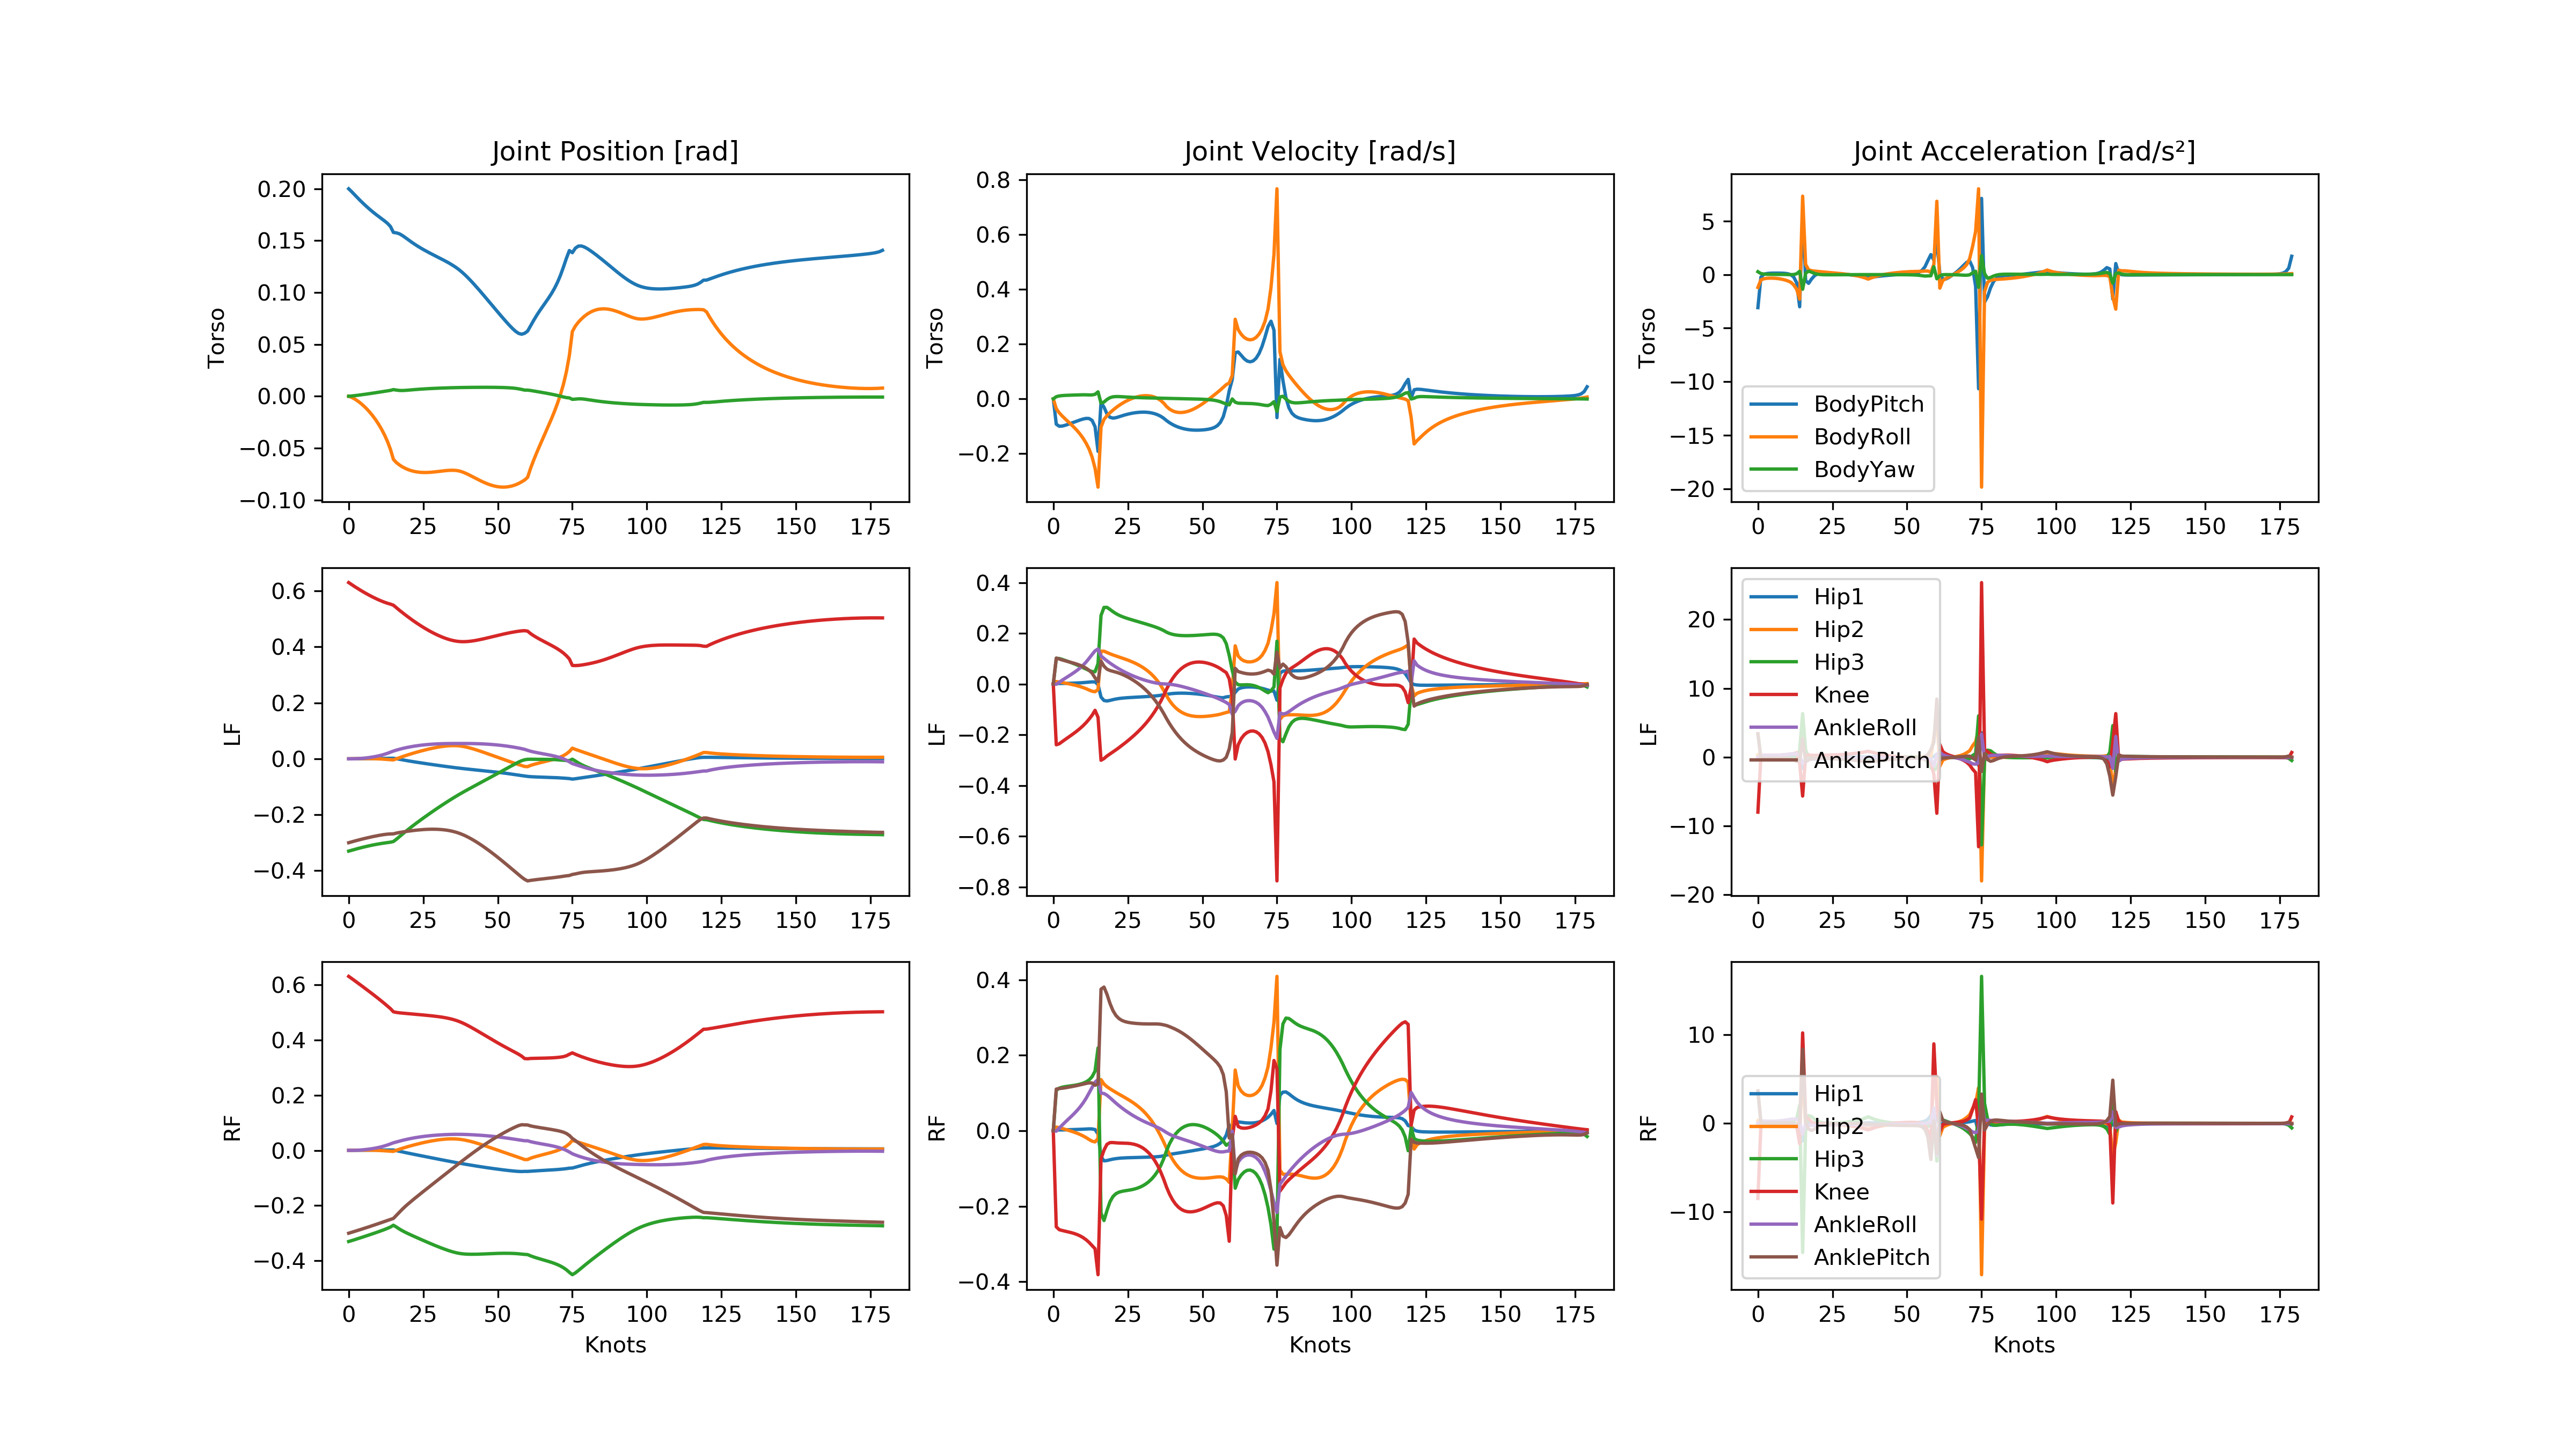
\includegraphics[width=.9\textwidth]{fig/walkDynamic/JointState}
\caption[Dynamic walking gait solution of the joint states.]{Dynamic walking gait solution of the joint states. Both joint velocities and acceleration show higher peaks along with higher joint deflections compared to the static walking, which is reasonable due to the higher walking speed.}
\label{fig:walkDynamic_JointState}
\end{figure} 

%\subsection{Dynamic Walking: Long Gait as Sequence of OC Problems}
%\subsection{Dynamic Walking: The Effect of Different Velocities}


\section{Evaluation of Contact Stability}\label{sec:BipedEvaluation}
This section evaluates, based on the presented dynamic walking gait from the previous section, the proposed approach of contact stability constrained DDP (\cref{c3}).

\subsection{Dynamically Balanced Walking Motion}
As detailed in \cref{sec:TheoryStability}, the central characteristic for dynamically balanced motions is that the \gls{CoP} or \gls{ZMP} remains within the \gls{SP}. The generic approach presented in \cref{c3} has been applied to the dynamic walking gait presented in the previous section. It utilizes the \gls{CoP} criterion for each contact surface and hence the motion can be called dynamically balanced only if the \gls{CoP} of each foot in contact stays within the according \gls{SP} along the whole motion. 

\cref{fig:walkDynamic_StabilityCoP100} shows the top view of the presented dynamic walking  gait. The rectangles correspond to the true-to-scale dimensions of the robot feet. For clarity, only the first and last \gls{DS} phase are visualized.  
The blue curve shows the time course of the resulting \gls{CoM} trajectory, with relevant points in time marked separately. Since the \gls{CoM} trajectory between lift-off and touch-down is largely outside the respective foot area, no static stability can be present, as expected. 
The orange and green crosses mark the time-dependent position of the \gls{CoP}s for both feet. It is evident that both \gls{CoP}s remain within the corresponding SP over the entire time course of the movement, which is why the movement can be classified as dynamically balanced. 

\subsection{Different Levels of CoP Restriction}
Although the dynamic walking motion is inherently balanced, it becomes clear from \cref{fig:walkDynamic_StabilityCoP100} that the \gls{CoP} partly lies \textit{on} or \textit{near} the border of the respective foot area. This effect can be attributed to the formulation of the \gls{CoP} cost function (\cref{eqn:CoPCostComputation}), which is defined to be zero whenever the \gls{CoP} lies within the given foot area and a quadratic penalization prevents the \gls{CoP} to leave the \gls{SP}. 
Theoretically, this formulation is sufficient to generate balanced motions. 
In practice however, it might be convenient for real-world experiments to consider a dedicated safety factor so that the \gls{CoP}s maintain a certain distance from the edge. With the presented \gls{CoP} cost function, this objective can be easily achieved by reducing the desired foot geometry. 
\cref{fig:walkDynamic_StabilityCoP50} shows the dynamic walking gait, where the \gls{CoP} inequality constraints are active for a \gls{SP} reduced to 50 percent of the original foot geometry. It becomes evident that also these more conservative contact stability constraints can be solved, which might be useful for the purpose of experimental validation. 

\begin{figure}[h!]
\centering	
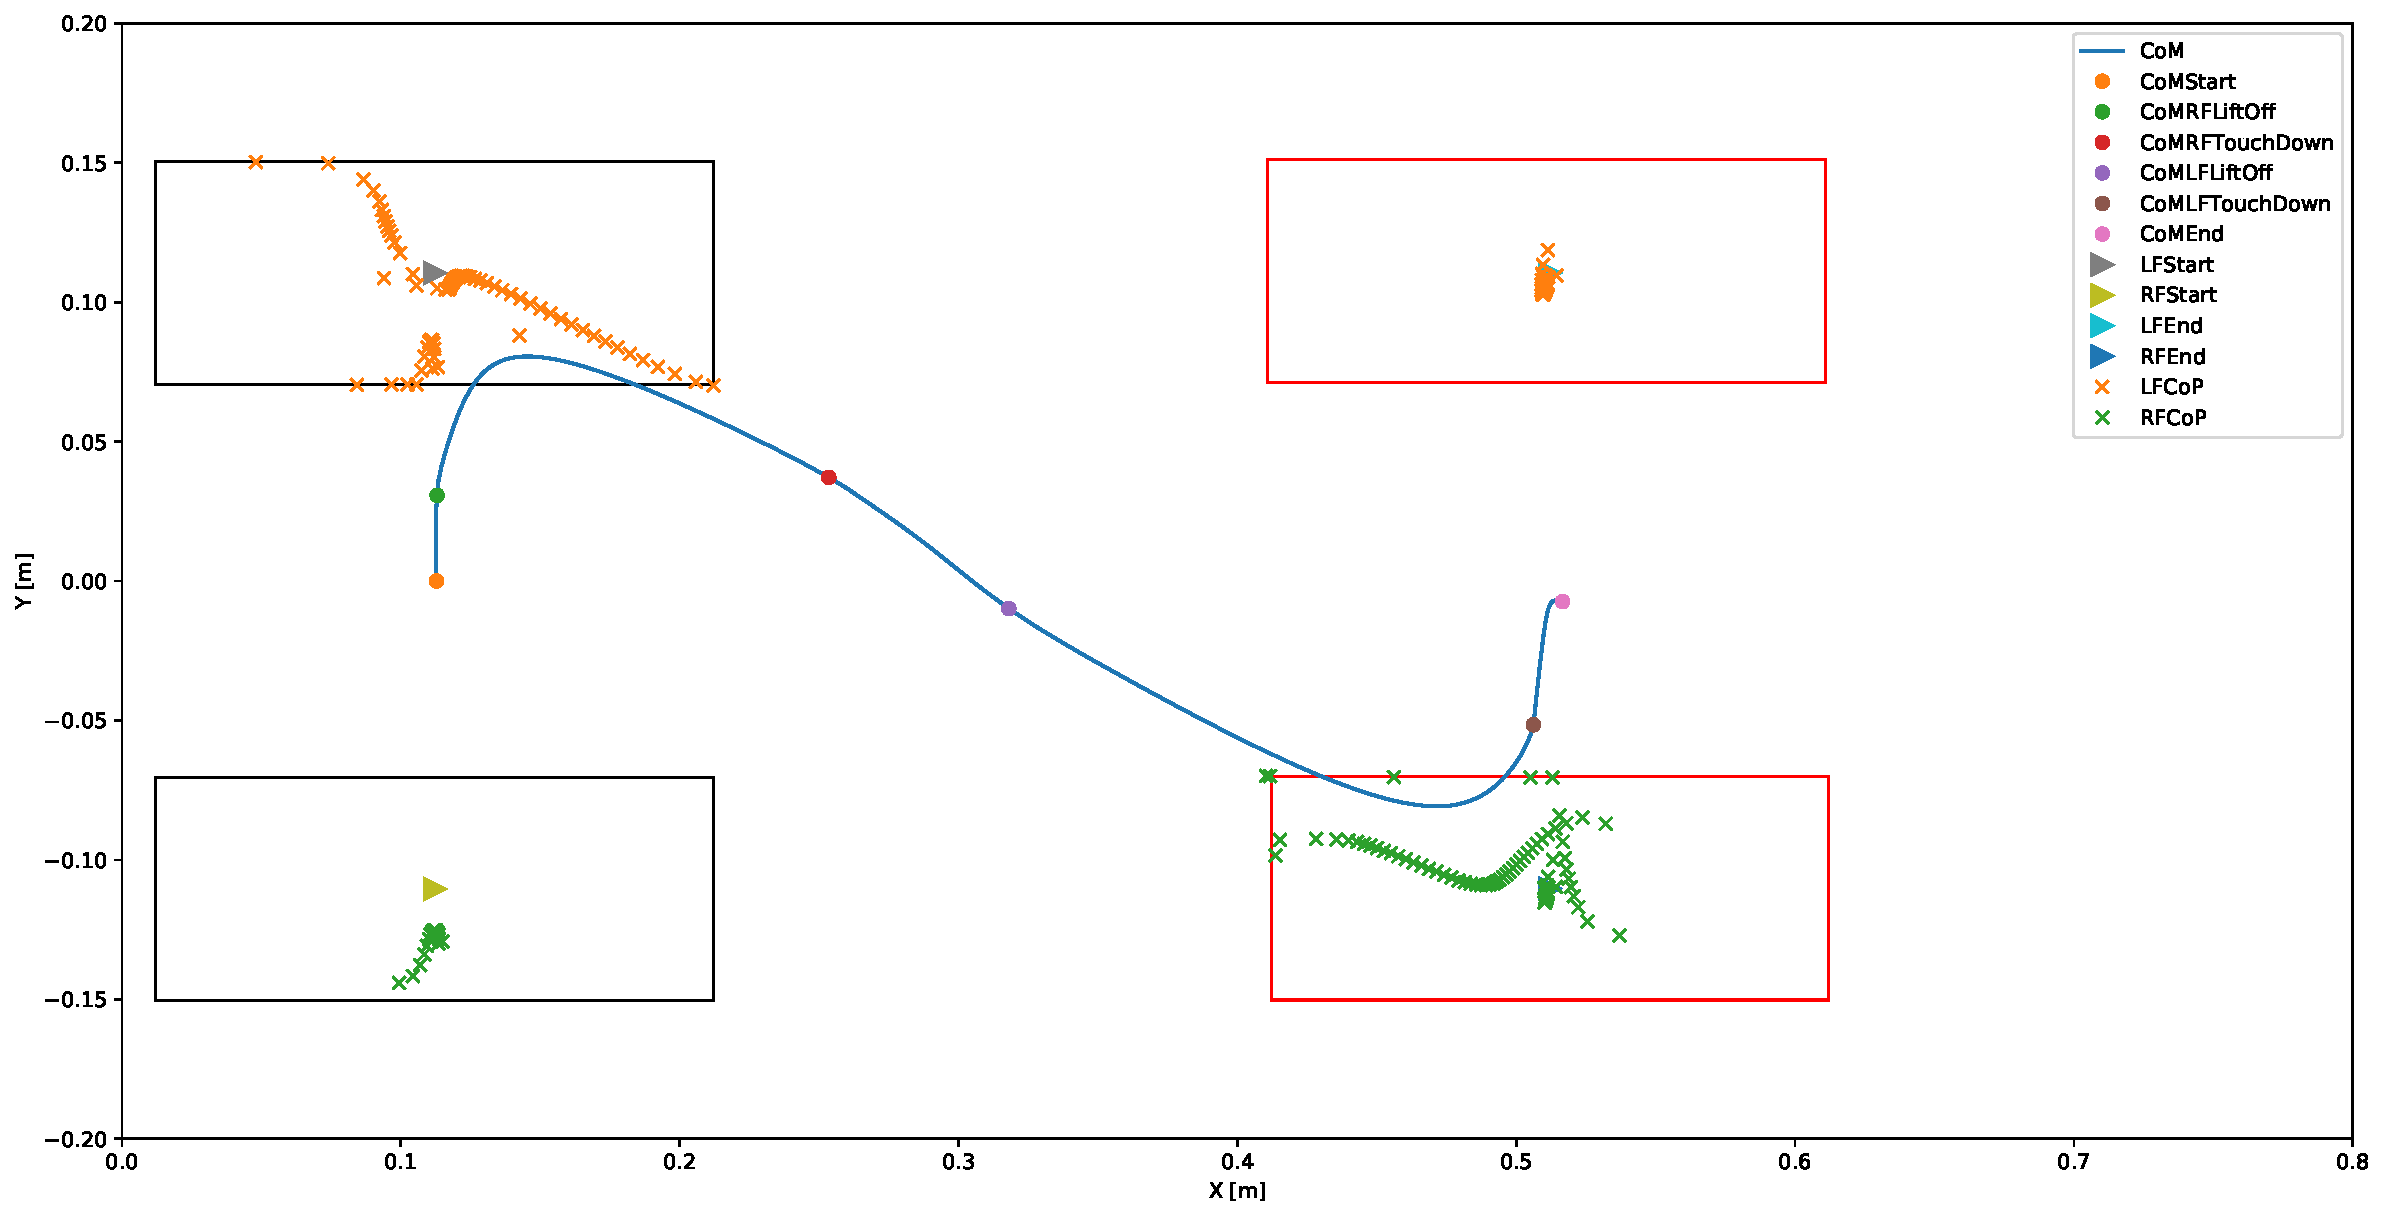
\includegraphics[width=1\textwidth]{fig/walkDynamic/StabilityAnalysis_CoP100}
\caption[Stability Analysis of the dynamic walking gait]{Stability Analysis of the dynamic walking gait. As both \gls{CoP}s remain within the corresponding SP, the movement can be classified as dynamically balanced. Hence, the functionality of the proposed contact stability constrained \gls{DDP} approach is verified.}
\label{fig:walkDynamic_StabilityCoP100}
\end{figure} 

\begin{figure}[h!]
\centering	
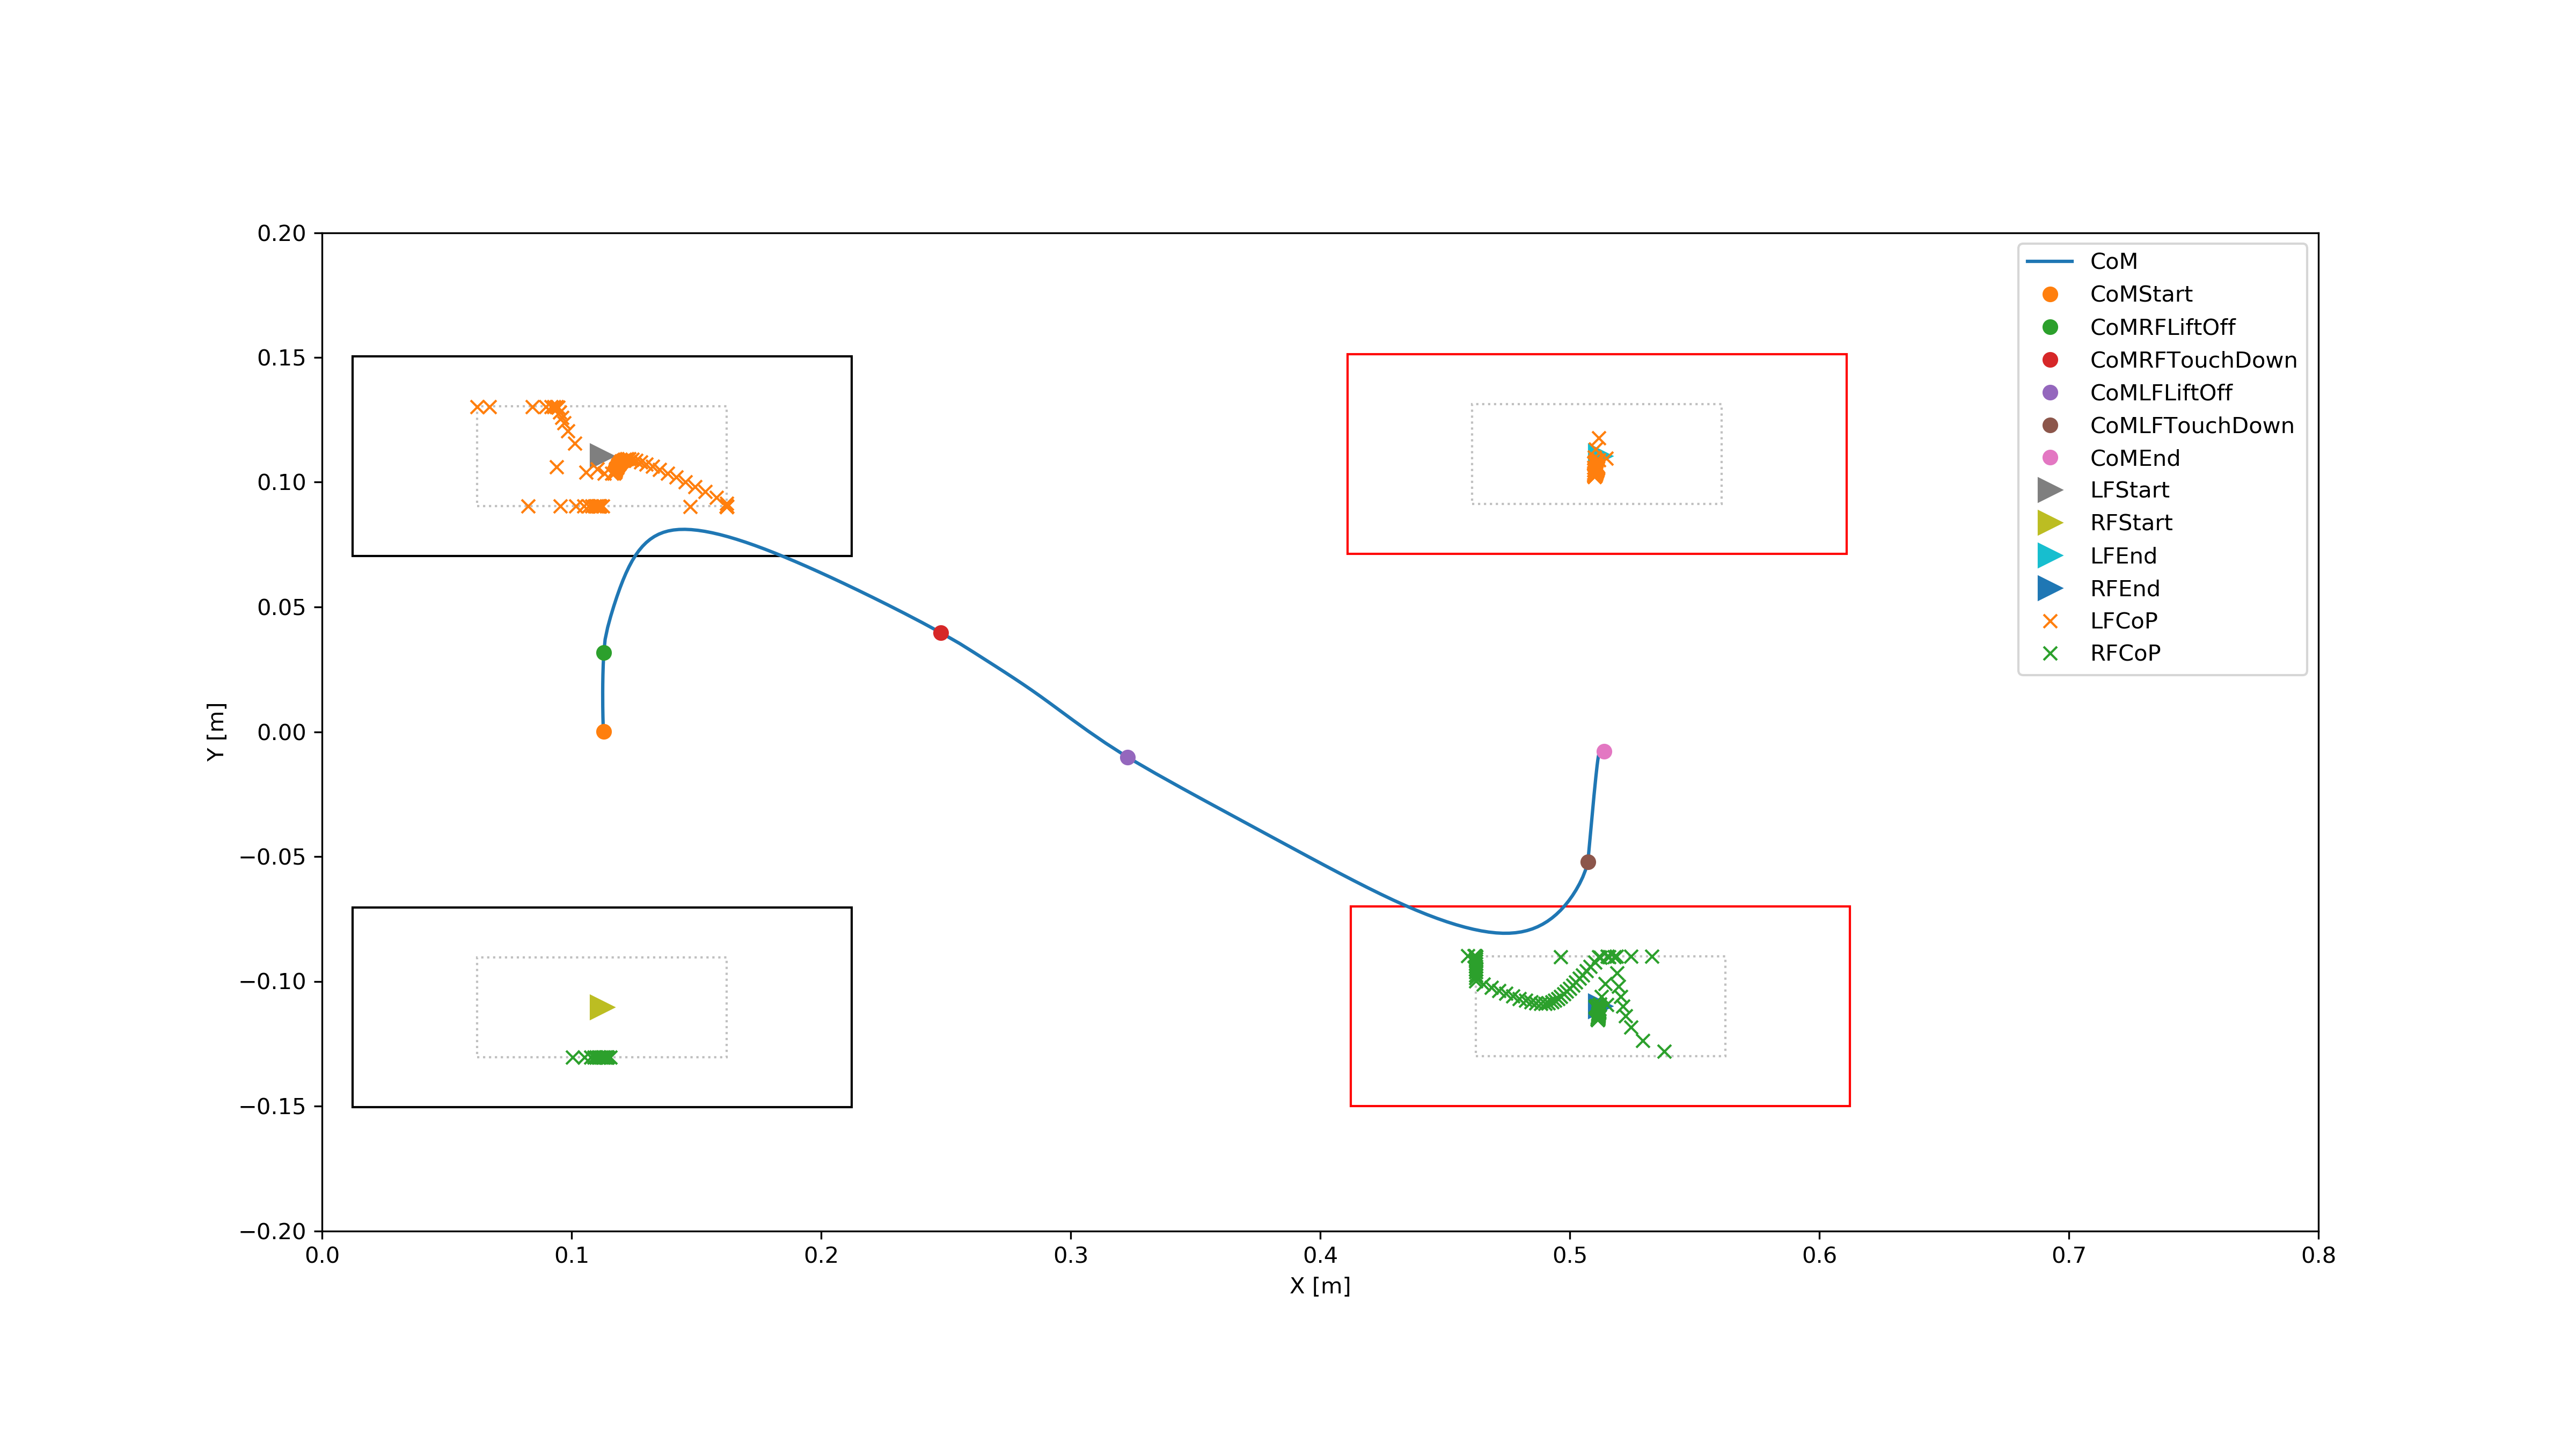
\includegraphics[width=1\textwidth]{fig/walkDynamic/StabilityAnalysis_CoP50}
\caption[Dynamic walking stability analysis with conservative \gls{CoP} restriction]{Stability analysis of the dynamic walking gait with a \gls{CoP} that is constrained in a \gls{SP} reduced by 50 percent. By this, the stability is more conservative, which may be convenient for real-world experiments}
\label{fig:walkDynamic_StabilityCoP50}
\end{figure}

In this section we have seen that the proposed contact stability constrained DDP produces motions that are dynamically balanced. In \cref{c6} we investigate if the generated motions can be tracked by a simple online stabilizer based on position control in joint space. Beforehand, in \cref{c5}, we explore the effect of the motion planning approach and physical system limits on highly dynamic movements.

























%%-----------------------------------------------------------------------------%
%                                                                             %
%    K A P I T E L   5                                                        %
%                                                                             %
%-----------------------------------------------------------------------------%

\chapter{Highly-Dynamic Movements}\label{c5}
This chapter presents an analysis of the proposed motion planning approach for highly-dynamic movements of the full-size humanoid RH5. To begin with, the central building blocks of the optimization problem are again briefly addressed. Then the simulation results for jumping tasks of increasing complexity are presented. Finally, an analysis of the maximal system performance based on the allowed joint and torque limits is presented.  


\section{Formulation of the Optimization Problem}
This section concisely summarizes the constraints of the \gls{OC} problem used to generate highly-dynamic movements as demonstrated in the following up section. 

The vertical jump formulation follows an optimization problem of the form described in \cref{eqn:optimizationProblem}. For performing multiple forward jumps over obstacles instead, we successively solve $P$ individual optimization problems of range $N$ for each jump. To this end, we formulate a multi-phase \gls{OC} problem as follows: 
\begin{equation}\label{eqn:optimizationProblemSequence}
\myM{X}^*,\myM{U}^*= 
\arg\min_{\mathbf{X},\mathbf{U}} \sum_{p=0}^{P}
\sum_{k=0}^{N-1} \int_{t_k}^{t_k+\Delta t} l_p(\mathbf{x},\mathbf{u})dt. 
\end{equation} 

We constrain the optimization based on the building blocks introduced in \cref{sec:BipedFormulation}. Precisely, we define a foot tracking cost $\Phi_1$ based on piecewise-linear functions to incorporate the basic jumping height and length. We apply the contact stability constrained \gls{DDP} (\cref{c3}) with dedicated cost functions for \gls{CoP} ($\Phi_3$) and friction cone ($\Phi_4$). Physical compliance is ensured via the torque bounds of the solver and joint limits costs $\Phi_5$. We use a \gls{CoM} tracking cost $\Phi_2$ only for the final stabilization of the motion. Additionally, torque minimization ($\Phi_6$) and posture regularization ($\Phi_7$) are optimized.

Biomechanical studies have shown that the effect of arm swinging is elementary for the performance in human jumping \cite{harman1990effects}. To this end, we also include the arms in the optimization for our jumping tasks. 
In order to account for the dynamic nature of the movements, it turned out to be useful to reduce the integration step size. We found a higher feasibility of the jumping tasks with an integration step size of 10ms compared to 30ms for the bipedal walking gaits (see \cref{sec:BipedSimulation}). Since we do not use a contact planner along with this work, the contact timings had to be chosen to approximately match the physic of flight phases. 
Highly dynamic movements are subject to higher impulse forces than is the case with walking movements. As described in \ref{sec:TheoryDDP}, \gls{DDP} relies on integration of the system dynamics in each step to obtain the states. The higher impulse forces then in turn cause numerical drifts of higher order in the contact constraints. This effect is visible as drifting of the support feet after touchdown. Through an extensive grid search, we found a set of valid Baumgarte gains that reduce these numerical drifts for highly-dynamic movements.

\section{Simulation Results for Increasing Task Complexity}
This section presents the simulation results for three case studies of highly-dynamic movements obtained by solving an optimization problem based on the description in the previous section. First, we study the task of vertically jumping upwards, then we investigate forward jumping and finally we explore a challenging sequence of multiple forward jumps over obstacles.

\subsection{A Simple Vertical Jump}
The analysis of a simple vertical jump is a good example to understand the underlying challenges highly-dynamic movements bring along in the context of numerical optimization.

\begin{table}[t]
\centering
\caption{Vertical jump characteristics and applied optimization constraints.}
\begin{tabular}{|ll|ll|}
\hline
\multicolumn{2}{|l|}{\textbf{Jump Characteristics}} & \multicolumn{2}{l|}{\textbf{Optimization Constraints}} \\ \hline
Jump height:& 10 cm 	& Tasks: 			& Foot ($\Phi_1$) \\ \hline
Total time:& 0.9 s 		& Stability:    & \gls{CoP} ($\Phi_3$), Friction Cone ($\Phi_4$)\\ \hline
Step size:& 0.01 s 	& Limits: 			& Torque ($\Phi_6$)\\ \hline
& 					& Regularization: 	& Posture ($\Phi_7$), Torque ($\Phi_8$)\\ \hline
\end{tabular}
\label{tab:jumpVertical}
\end{table}

The vertical jumping task (see \cref{tab:jumpVertical}) consists of five phases as depicted in \cref{fig:jumpVertical_Snaps}. From the initial position (a), a descending into the jump (b) takes place. Then, an upward motions accelerates the base until the take off (c). The symmetrical flight phase (d) is ended with a touch down (e) followed by a pose recovery (f). 

\begin{figure}[h!]
\begin{subfigure}{.16\textwidth}
	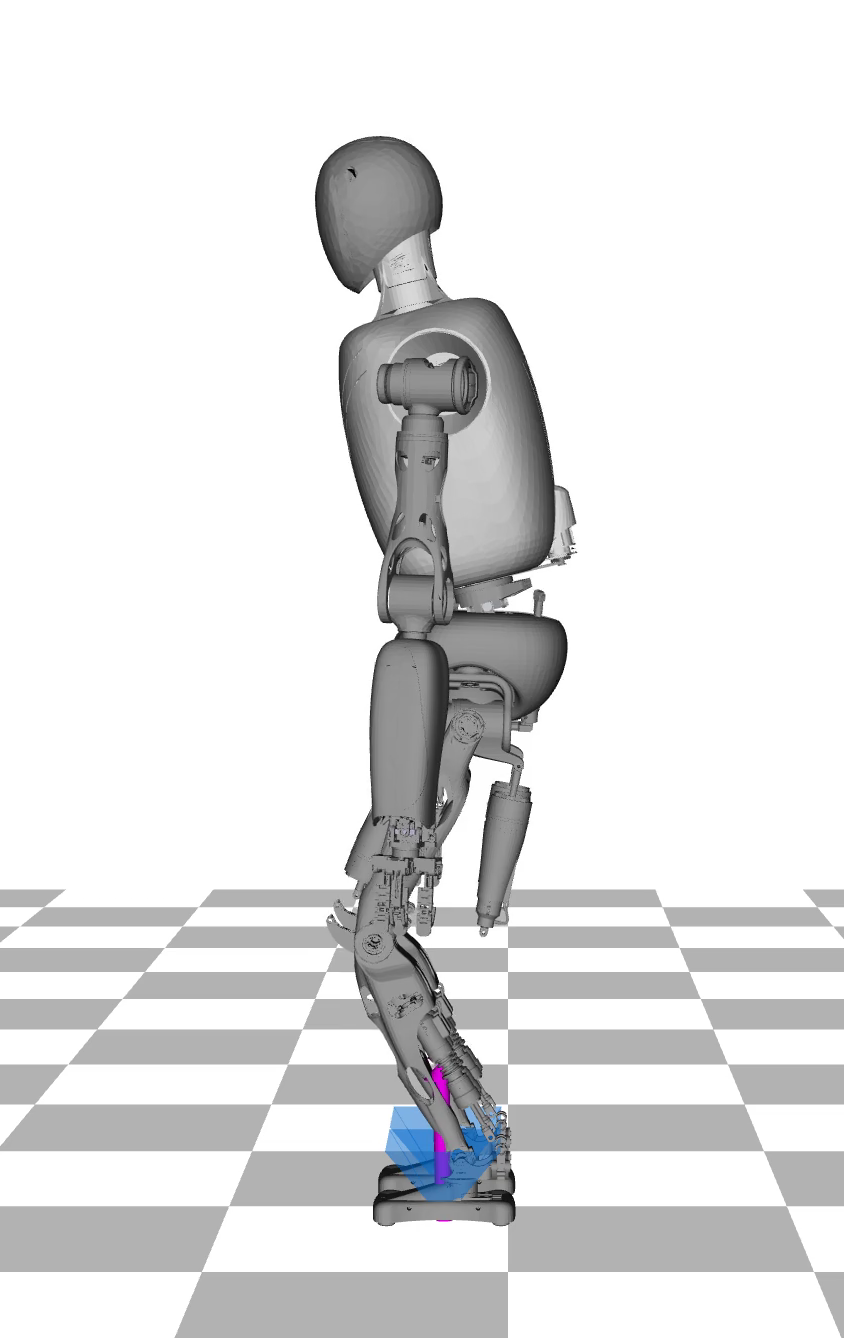
\includegraphics[width=1\linewidth]{fig/jumpVertical/snaps/1x}
	\caption{}
	\end{subfigure}%
\begin{subfigure}{.16\textwidth}
	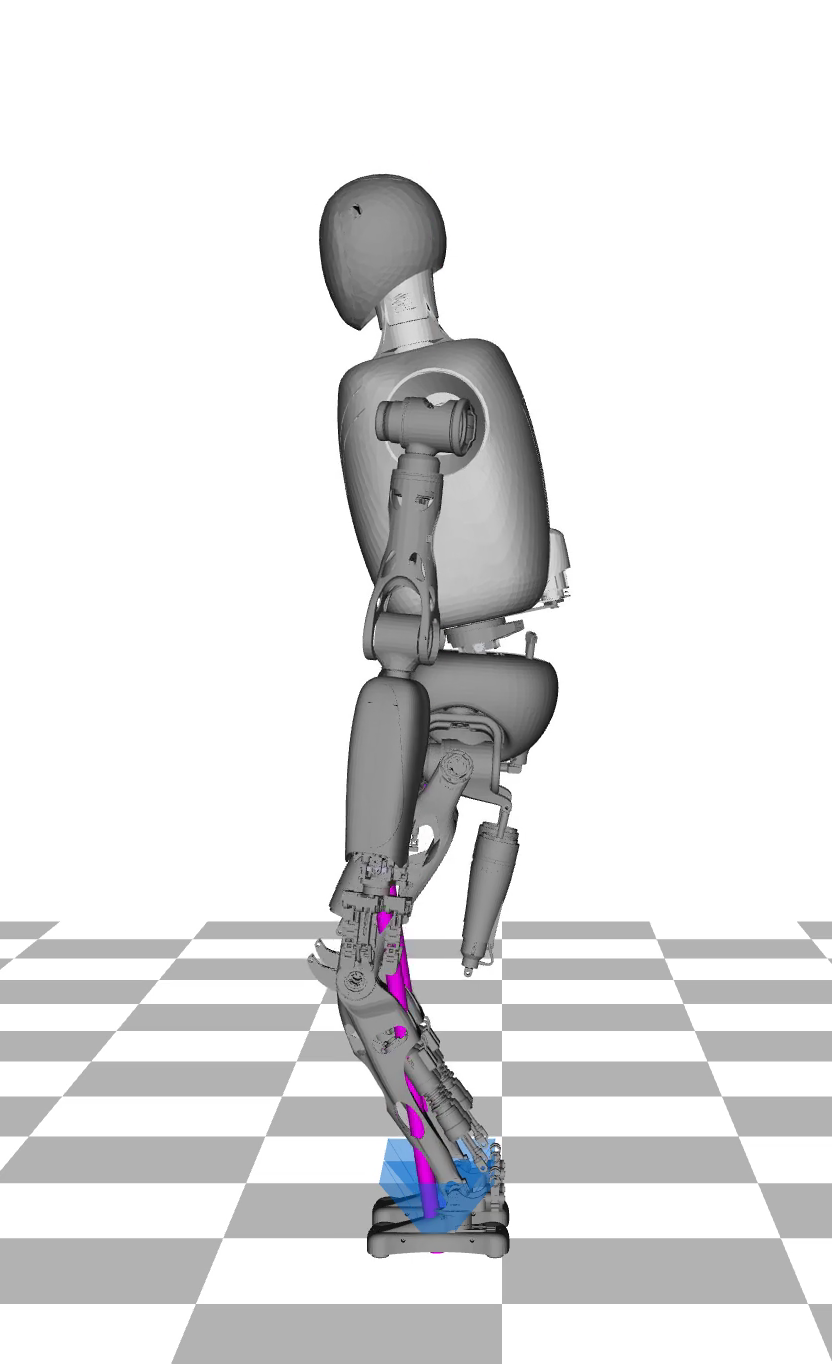
\includegraphics[width=1\linewidth]{fig/jumpVertical/snaps/2x}
	\caption{}
\end{subfigure}%
\begin{subfigure}{.16\textwidth}
	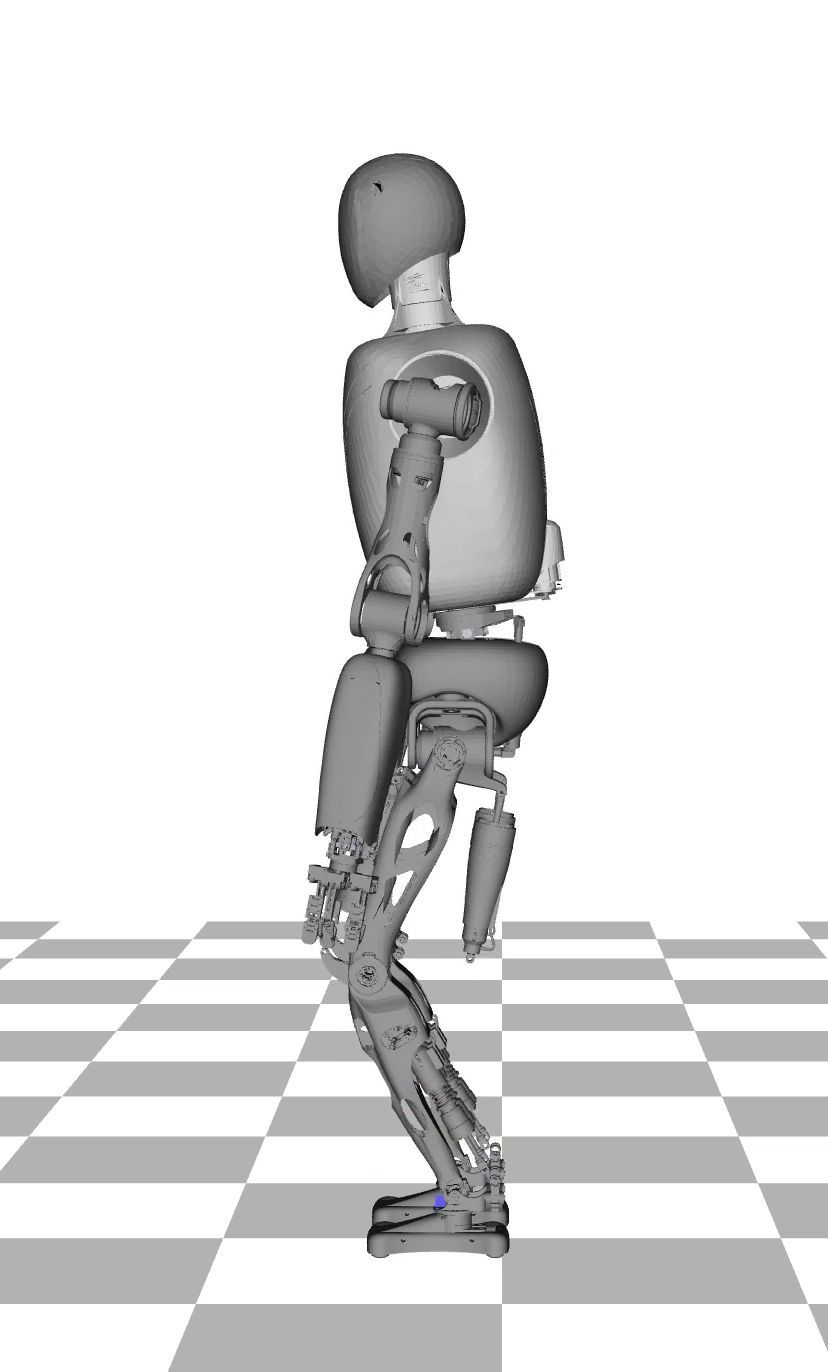
\includegraphics[width=1\linewidth]{fig/jumpVertical/snaps/3x}
	\caption{}
	\end{subfigure}%
\begin{subfigure}{.16\textwidth}
	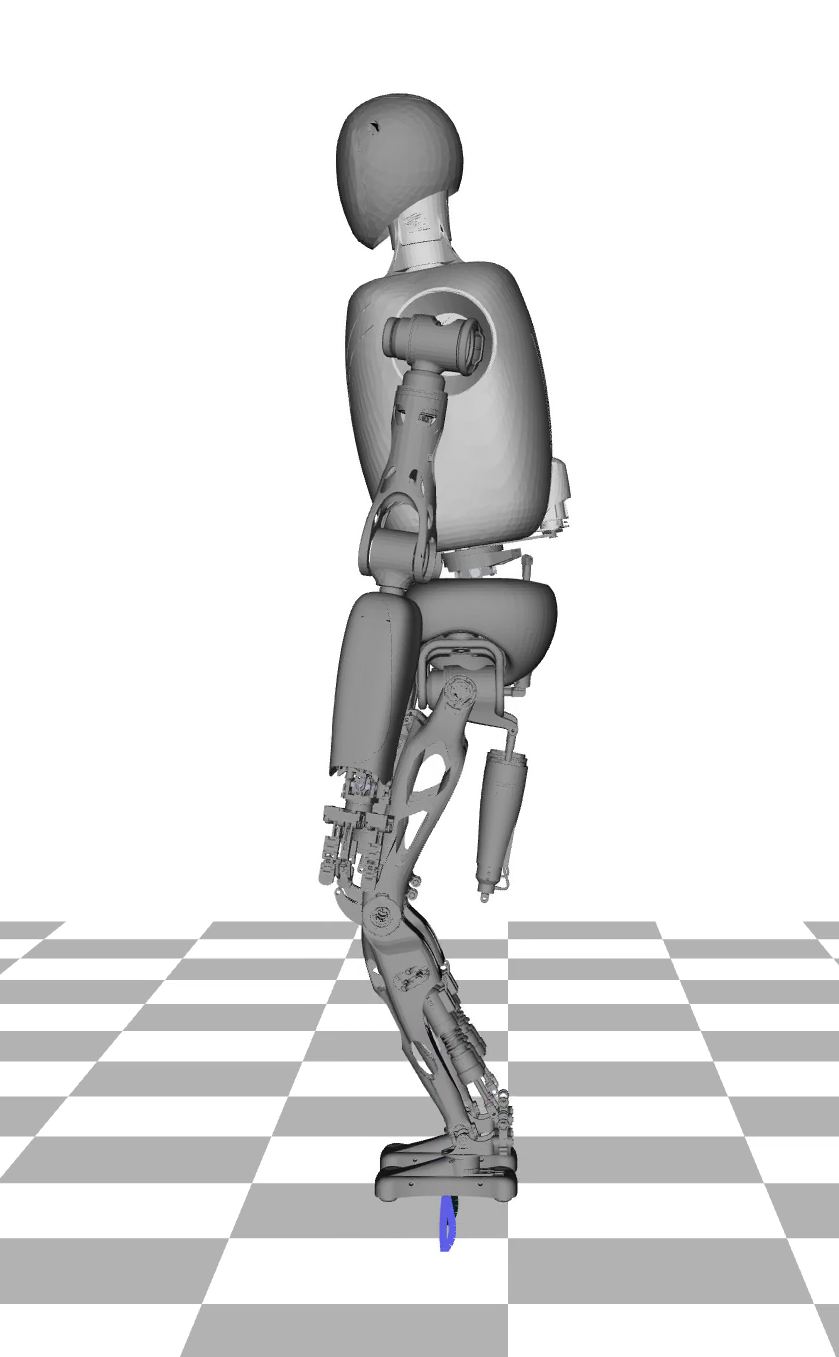
\includegraphics[width=1\linewidth]{fig/jumpVertical/snaps/4x}
	\caption{}
\end{subfigure}%
\begin{subfigure}{.16\textwidth}
	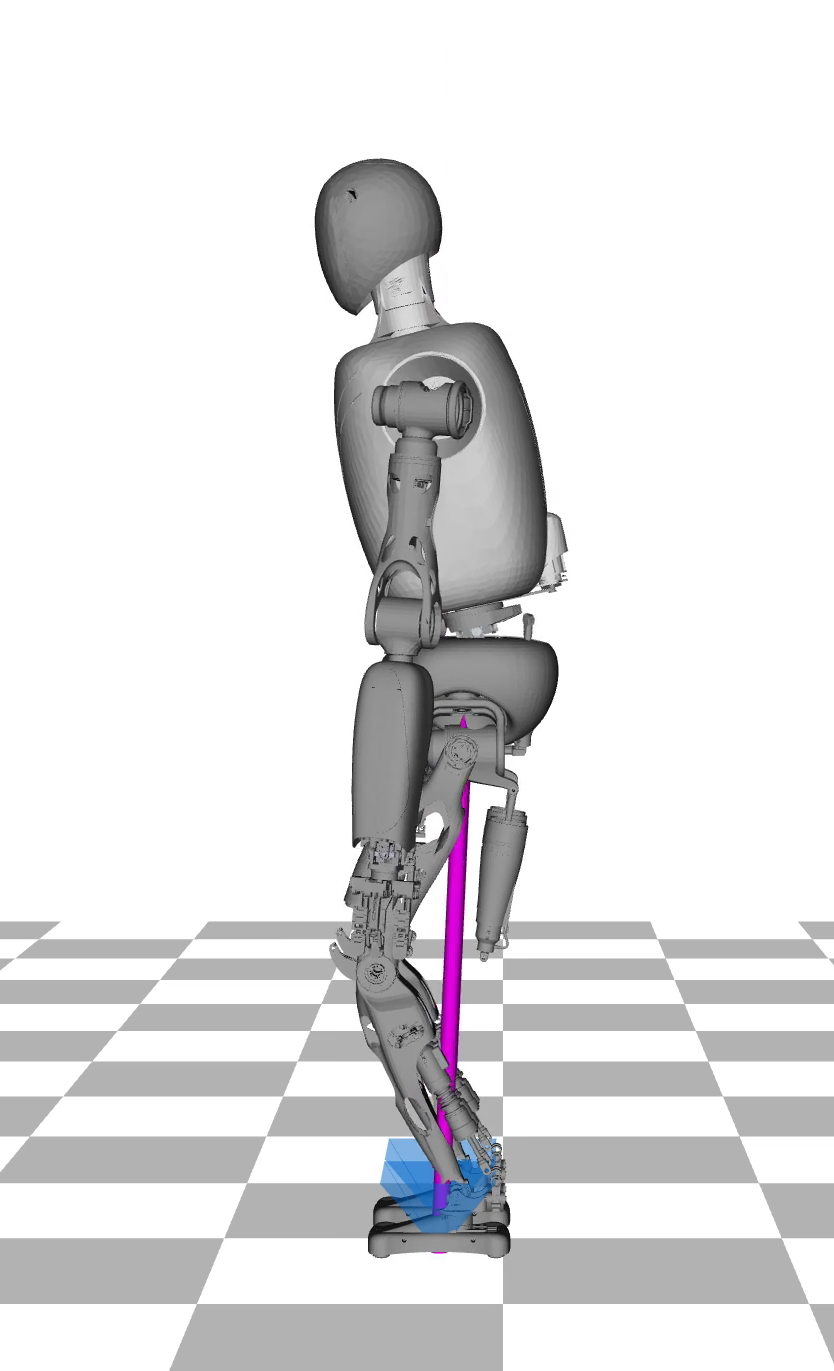
\includegraphics[width=1\linewidth]{fig/jumpVertical/snaps/5x}
	\caption{}
	\end{subfigure}%
\begin{subfigure}{.16\textwidth}
	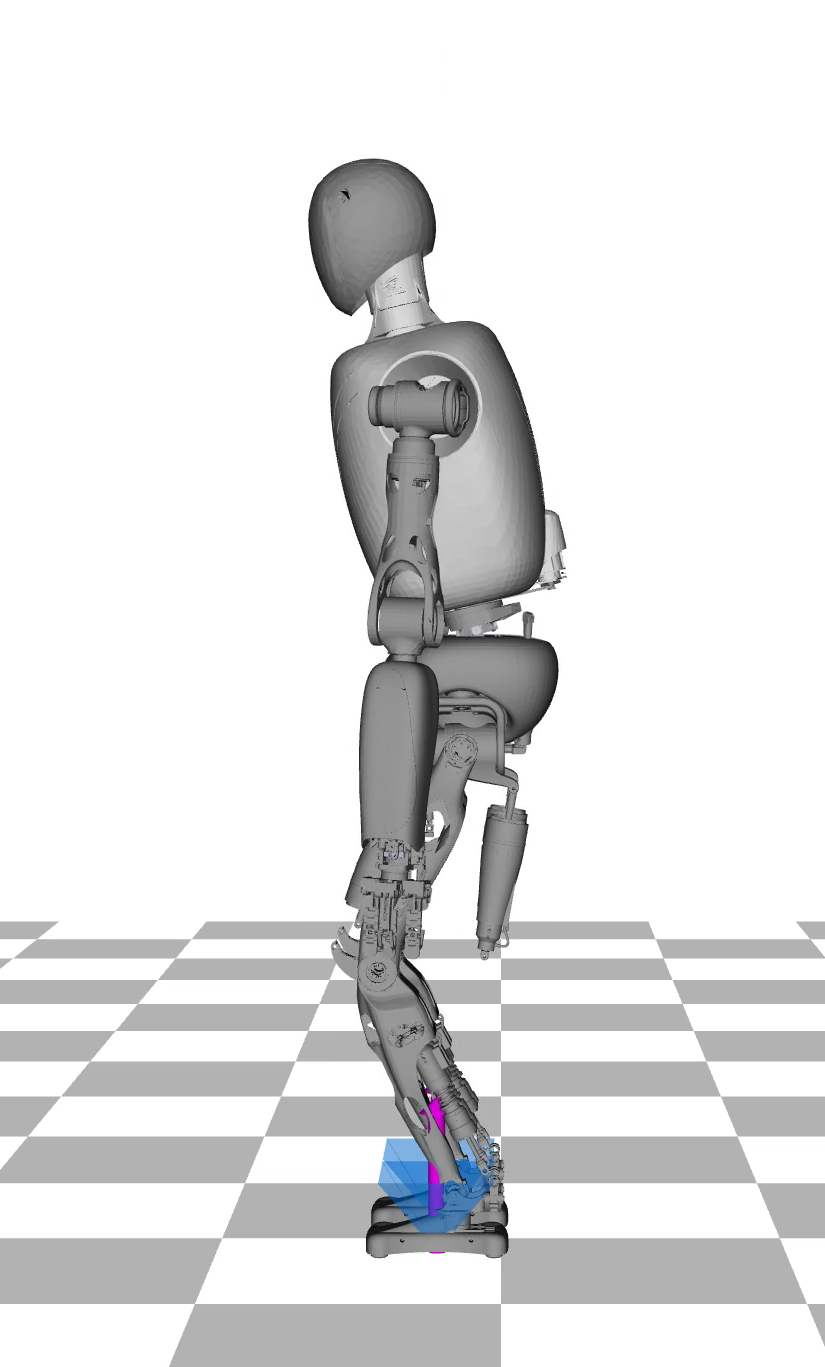
\includegraphics[width=1\linewidth]{fig/jumpVertical/snaps/6x}
	\caption{}
\end{subfigure}%
\caption{A simple vertical jump.}
\label{fig:jumpVertical_Snaps}
\end{figure} 

\cref{fig:jumpVertical_JointState} provides insights in the dynamic nature of the motion. As can be seen, the joint positions stay within reasonable ranges. However, velocity peaks at the take off exceed the maximum joint velocities of the body pitch and knee joints by a factor of two and four, respectively. This effect is plausible, since both the knee deflection as well as the torso swing are essential for a jump. Consequently, the short time horizon of the jump requires high peak velocities in these task-relevant joints. 

\begin{figure}[h!]
\centering	
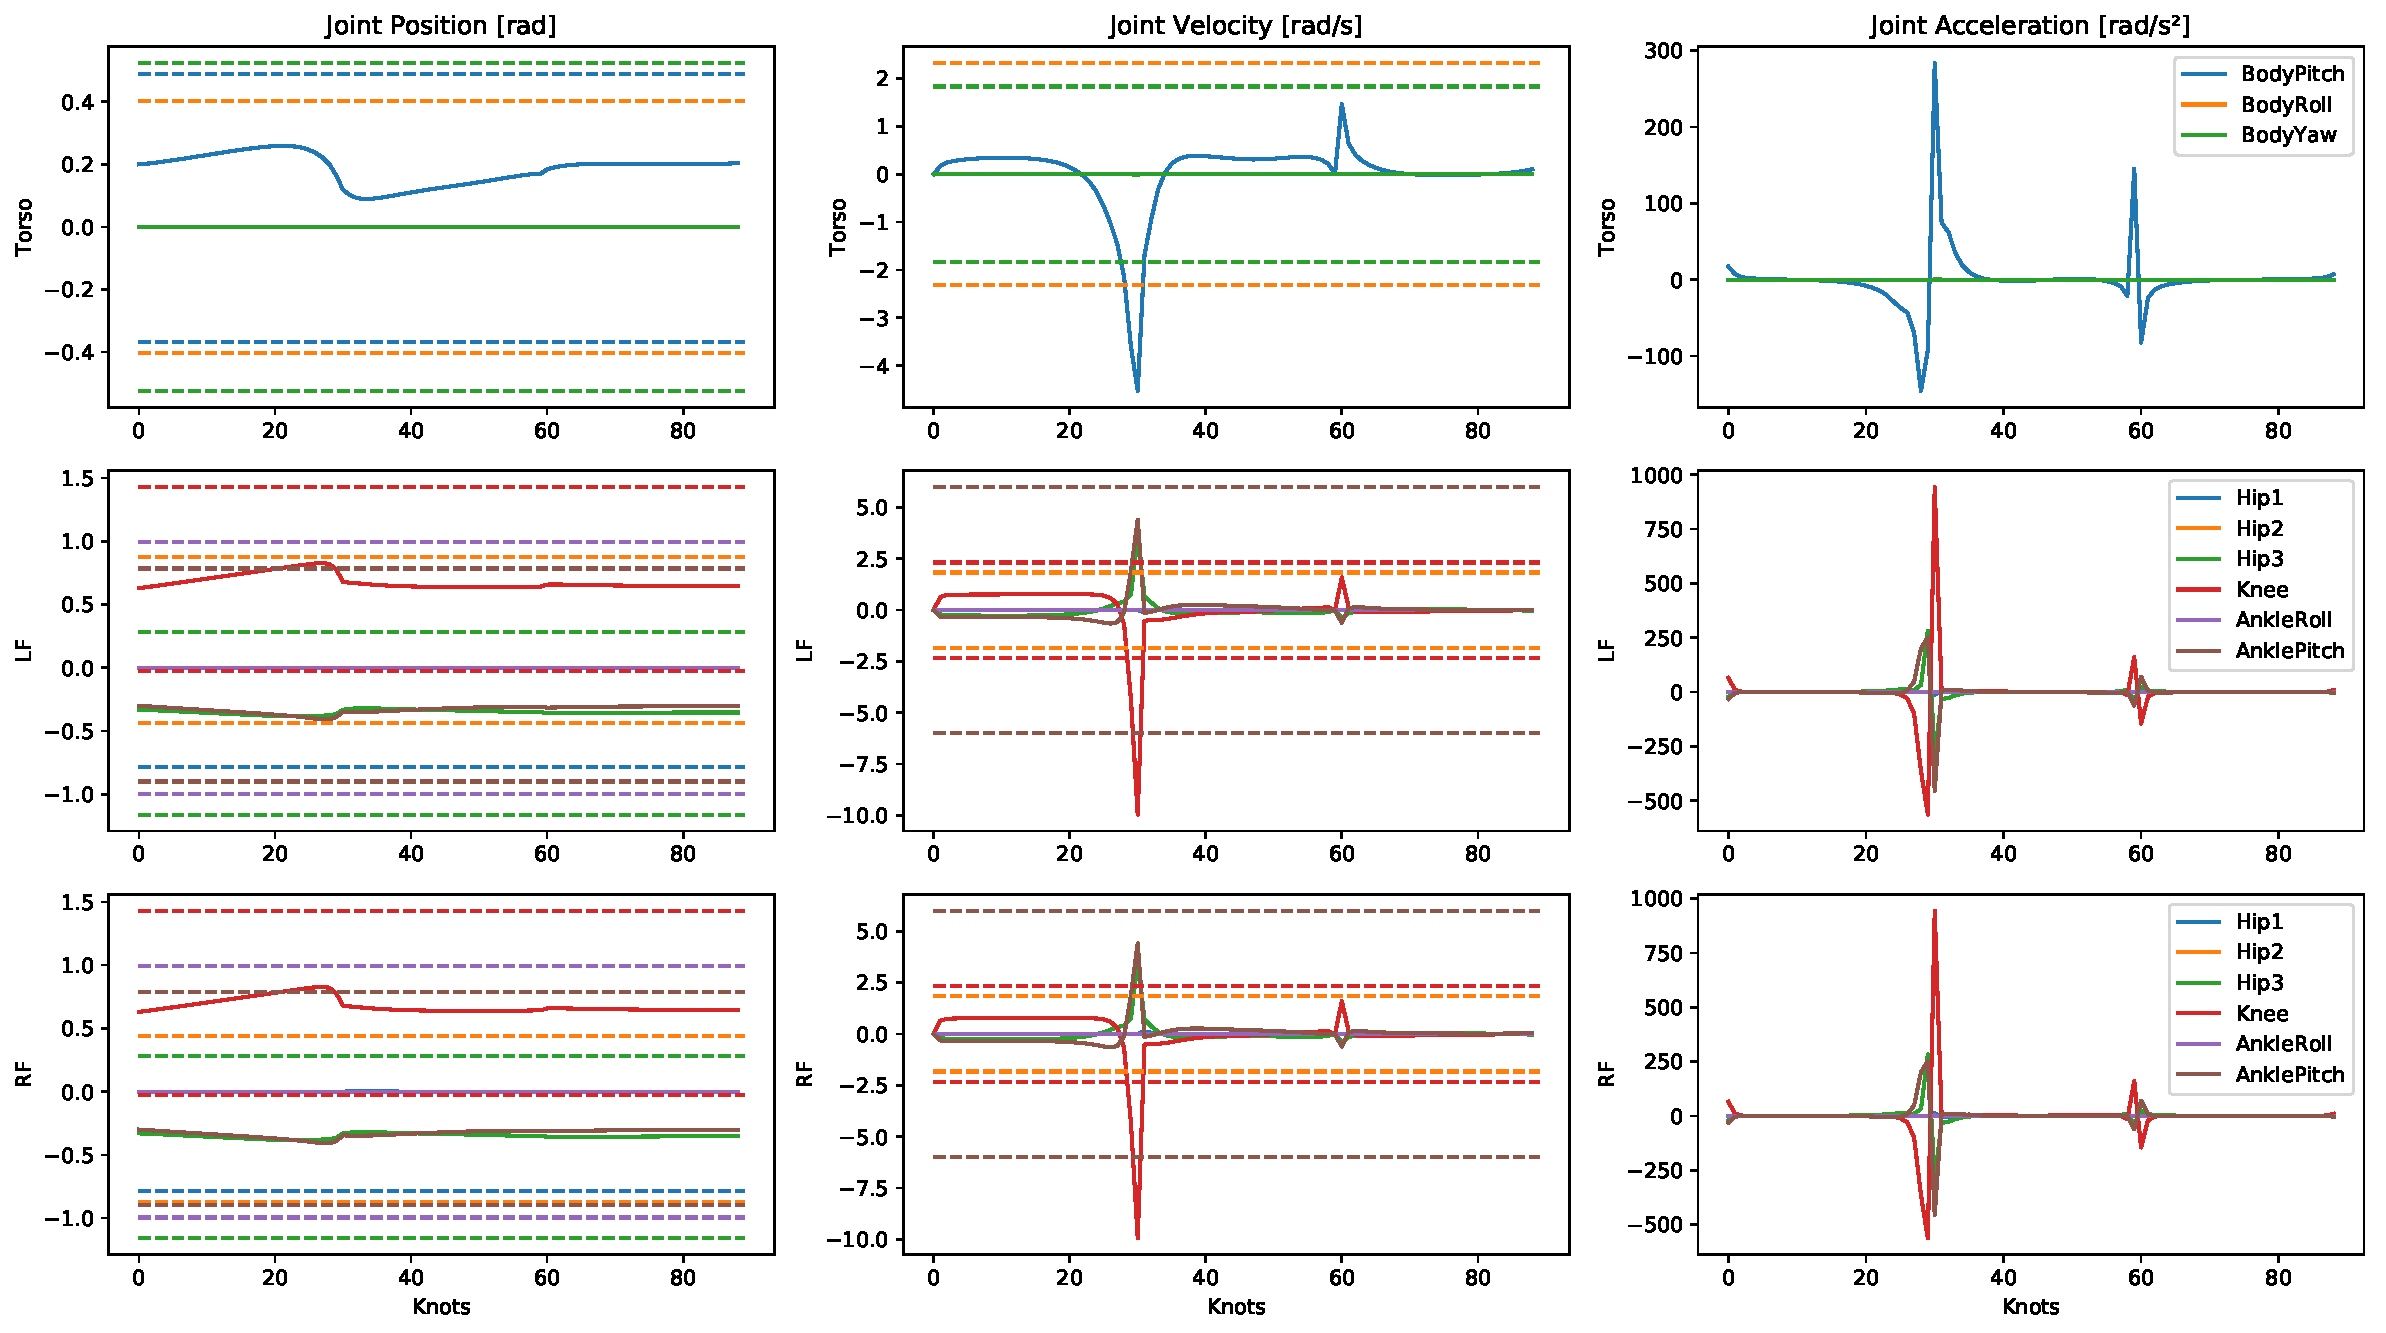
\includegraphics[width=1\textwidth]{fig/jumpVertical/JointState}
\caption{Vertical jump solution of the joint states with according joint limits visualized as dashed lines. The maximum velocities of the body pitch and knee joints turn out to be insufficient for the highly-dynamic take off.}
\label{fig:jumpVertical_JointState}
\end{figure} 

A similar observation applies to the joint torques as shown in \cref{fig:jumpVertical_JointTorques}. Although the solver prevents the body pitch and knee torques to exceed the limits in this case, it becomes evident that maximum torques for these joints are necessary over longer time horizons. Such continuous loads should be avoided as far as possible in order to guarantee the durability of the robotic system.

\begin{figure}[h!]
\centering	
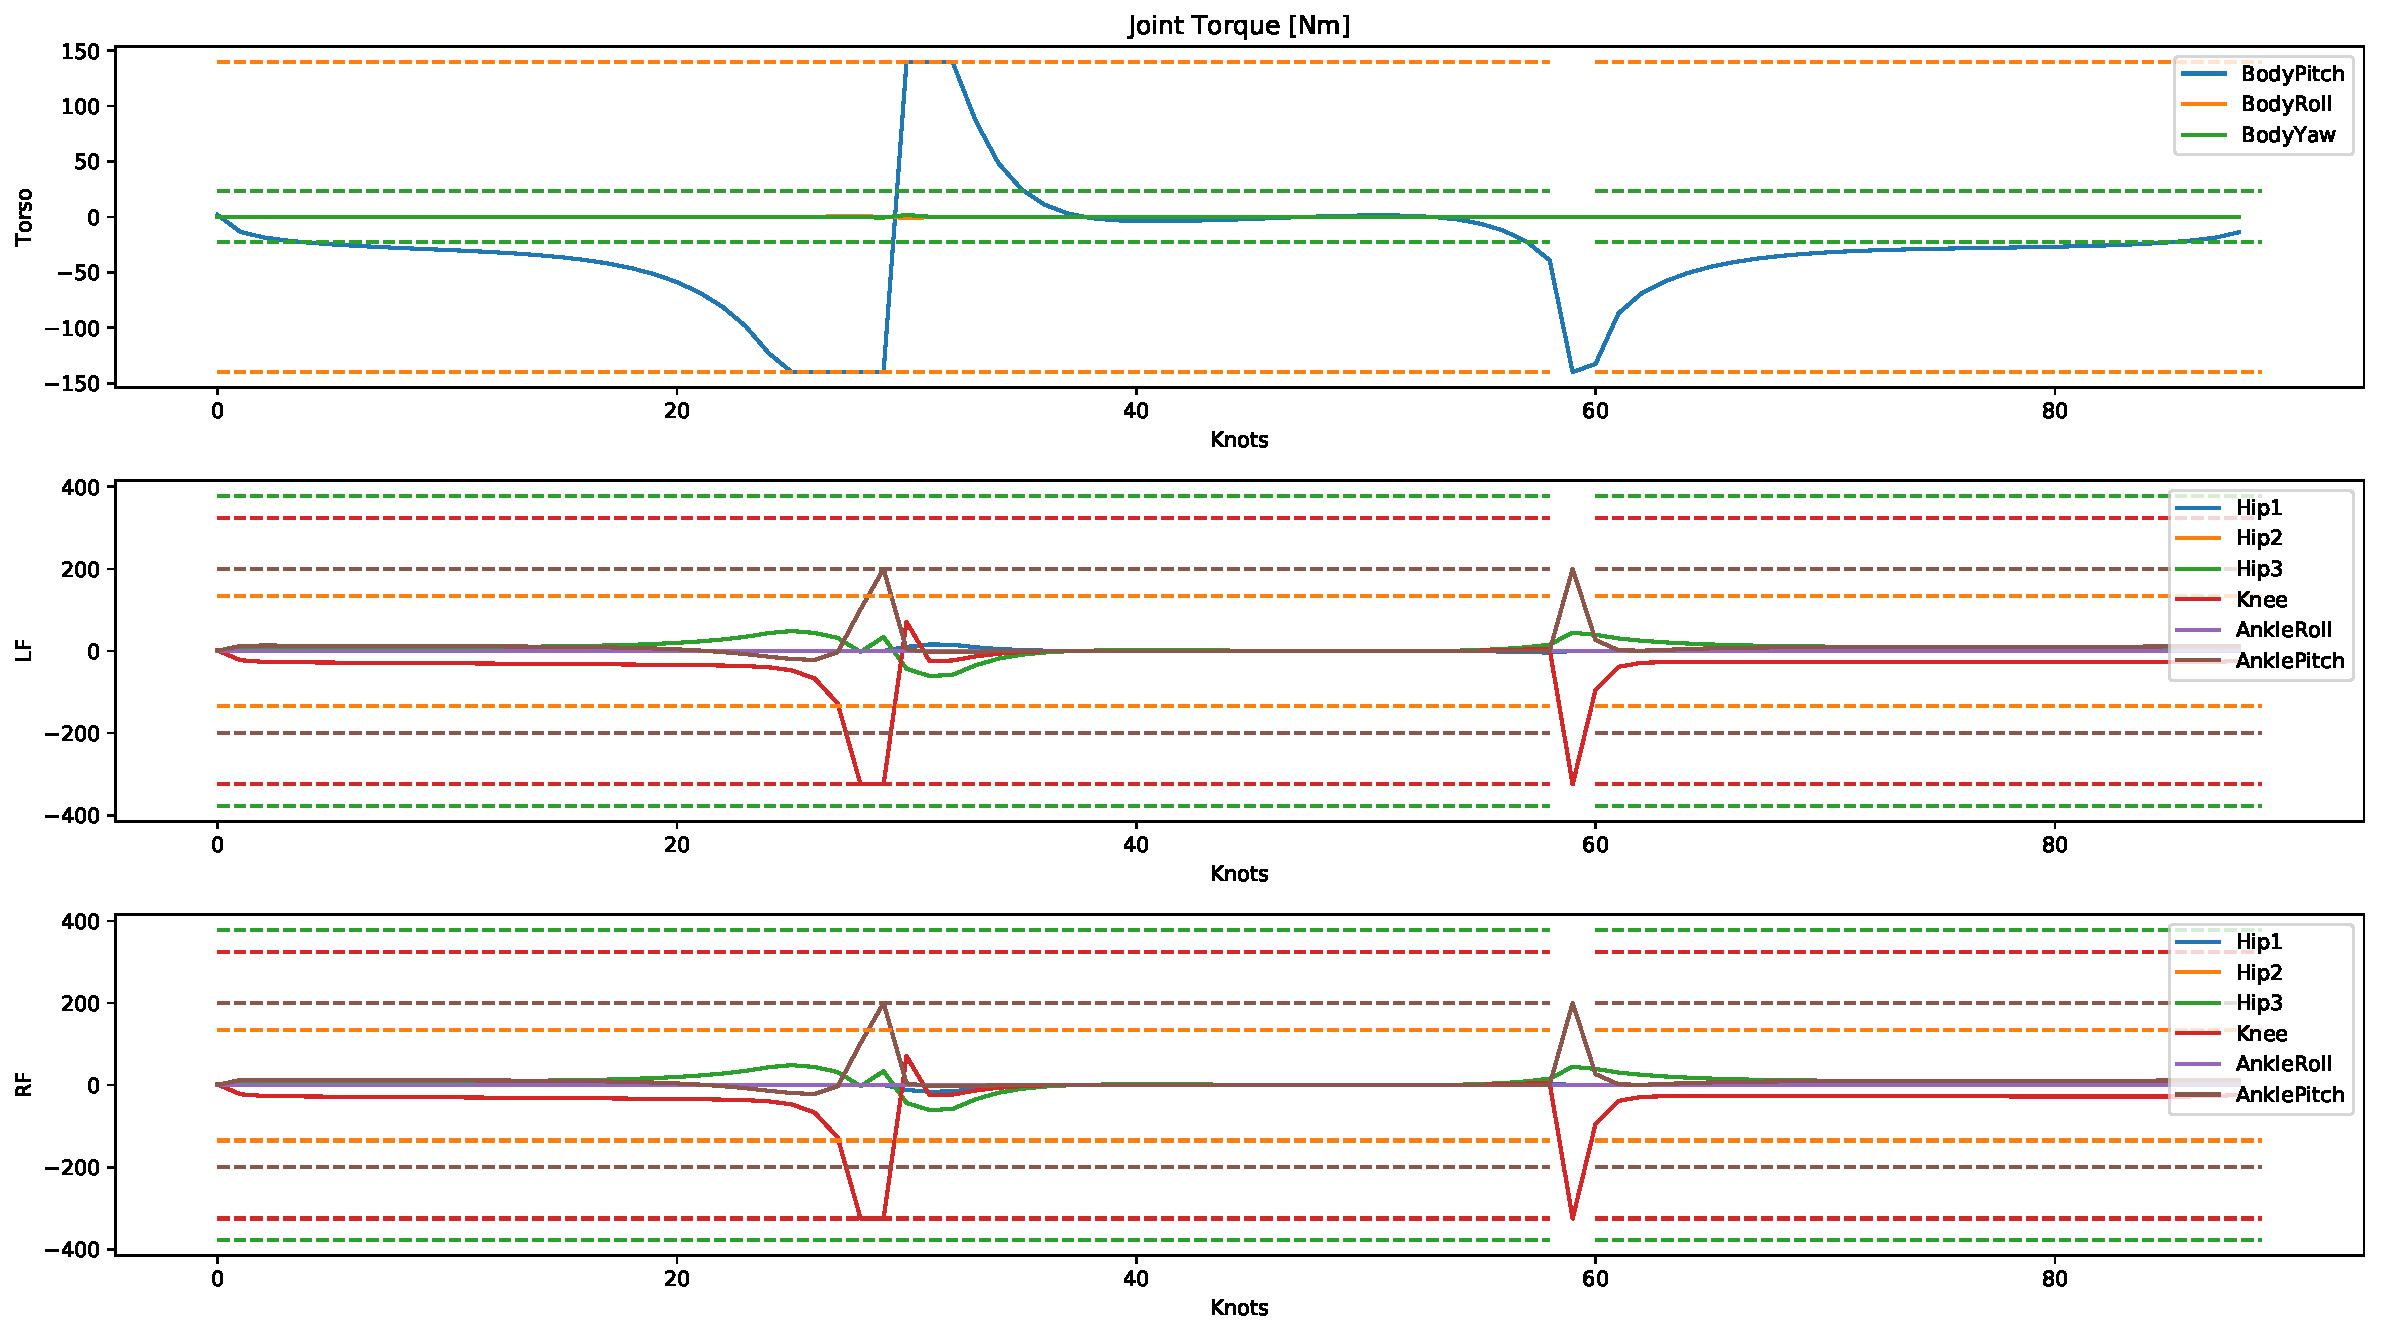
\includegraphics[width=1\textwidth]{fig/jumpVertical/JointTorques}
\caption{Vertical jump solution of the joint torques with according motor limits visualized as dashed lines. The solver prevents the body pitch and knee torques to exceed the limits, but still maximum torques are required for these joints over longer time horizons.}
\label{fig:jumpVertical_JointTorques}
\end{figure} 

\subsection{A Simple Forward Jump}
Focus of investigation is a more dynamic forward jump to study the effect of increasing task complexity on the contact forces and stability.

\cref{tab:jumpForward} summarizes the characteristics and optimization constraints. The forward jumping problem consists of the same five locomotion phases as the vertical jump described previously (see \cref{fig:jumpForward_Snaps}). 
We can draw similar conclusions regarding the physical compliance of the system, namely appropriate joint position ranges and torque limits, but insufficient maximal velocities for the body pitch and knee joints. 

\begin{table}[t]
\centering
\caption{Forward jump characteristics and applied optimization constraints.}
\begin{tabular}{|ll|ll|}
\hline
\multicolumn{2}{|l|}{\textbf{Jump Characteristics}} & \multicolumn{2}{l|}{\textbf{Optimization Constraints}} \\ \hline
Jump length:& 30 cm 	& Tasks: 			& Foot ($\Phi_1$) \\ \hline
Jump height:& 10 cm 	& Stability: 		& \gls{CoP} ($\Phi_3$), Friction Cone ($\Phi_4$)\\ \hline
Total time:& 0.9 s  	& Limits: 			& Torque ($\Phi_6$)\\ \hline
Step size:& 0.01 s   & Regularization: 	& Posture ($\Phi_7$), Torque ($\Phi_8$)\\ \hline
\end{tabular}
\label{tab:jumpForward}
\end{table}

\begin{figure}[h!]
\begin{subfigure}{.16\textwidth}
	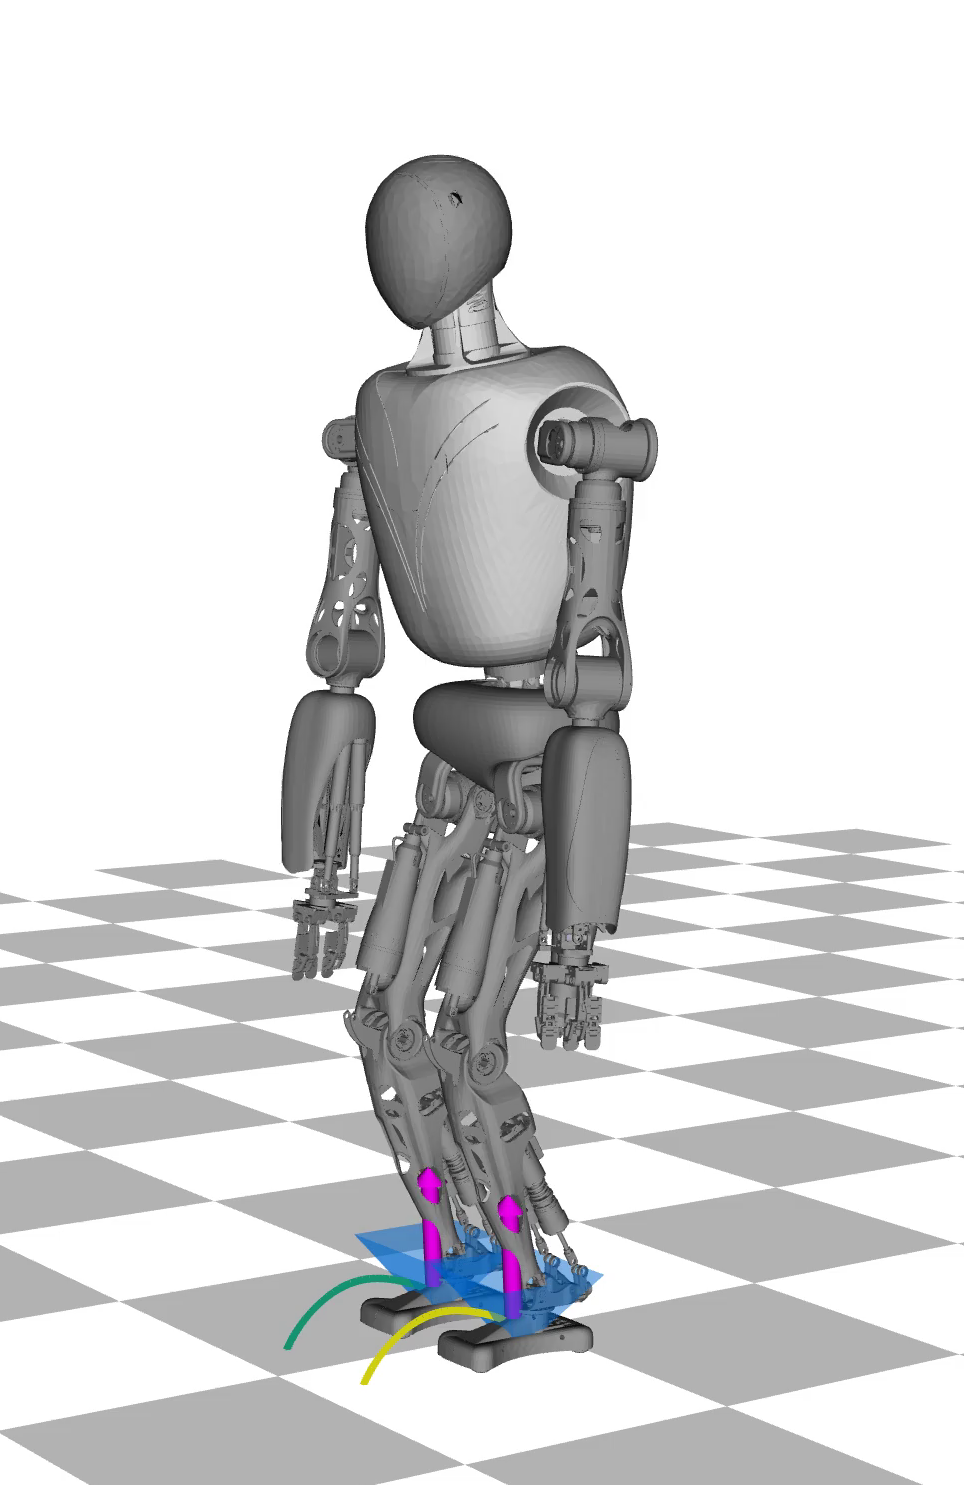
\includegraphics[width=1\linewidth]{fig/jumpForward/snaps/1x}
	\caption{}
	\end{subfigure}%
\begin{subfigure}{.16\textwidth}
	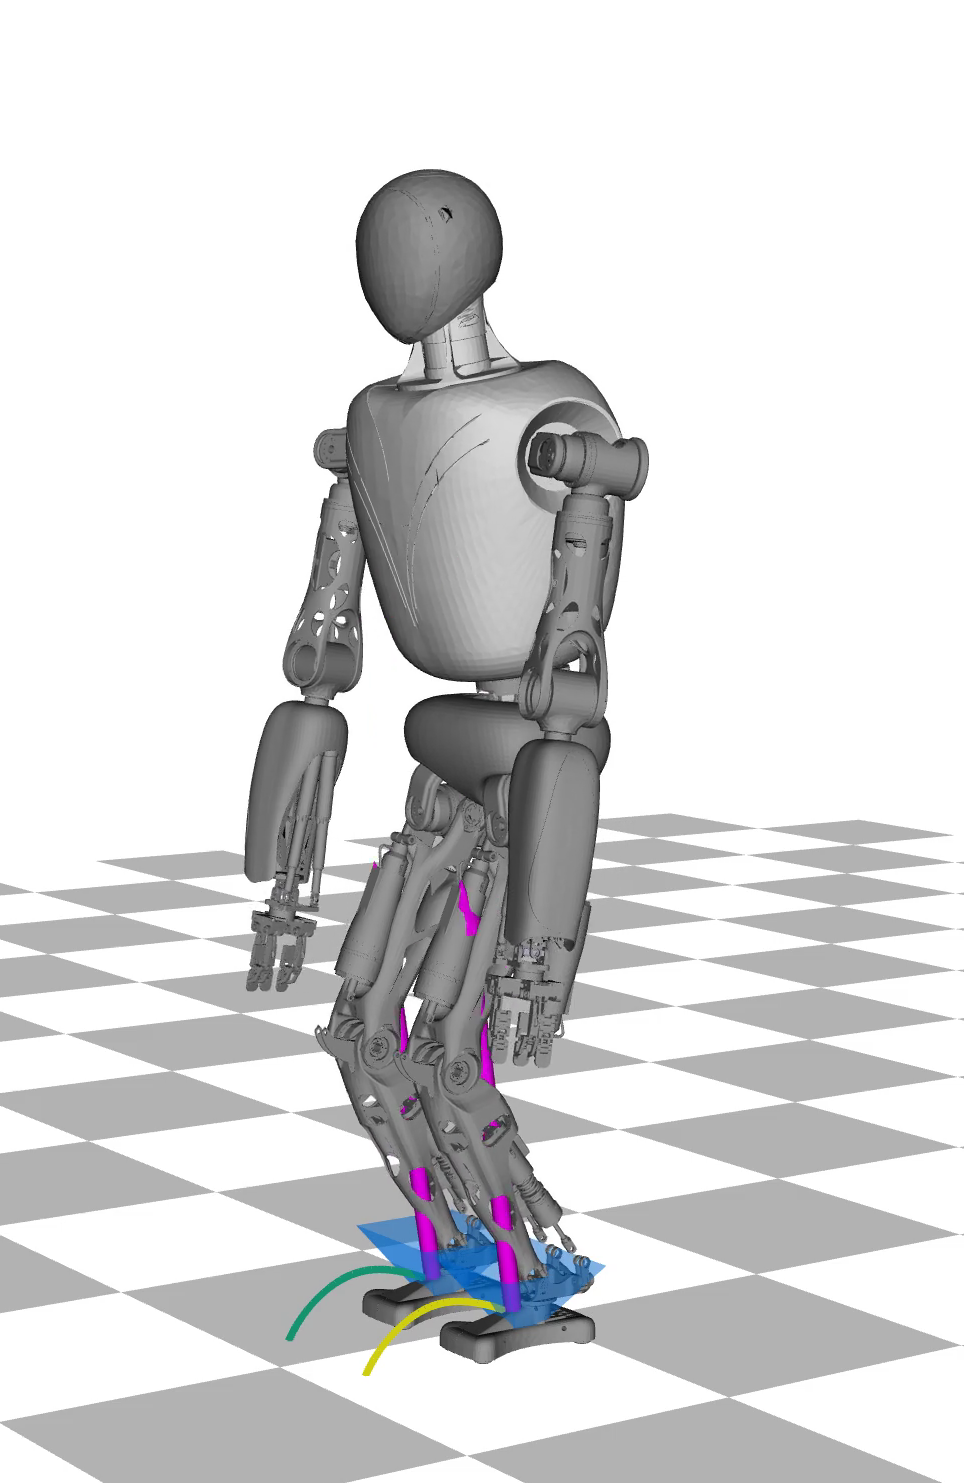
\includegraphics[width=1\linewidth]{fig/jumpForward/snaps/2x}
	\caption{}
\end{subfigure}%
\begin{subfigure}{.16\textwidth}
	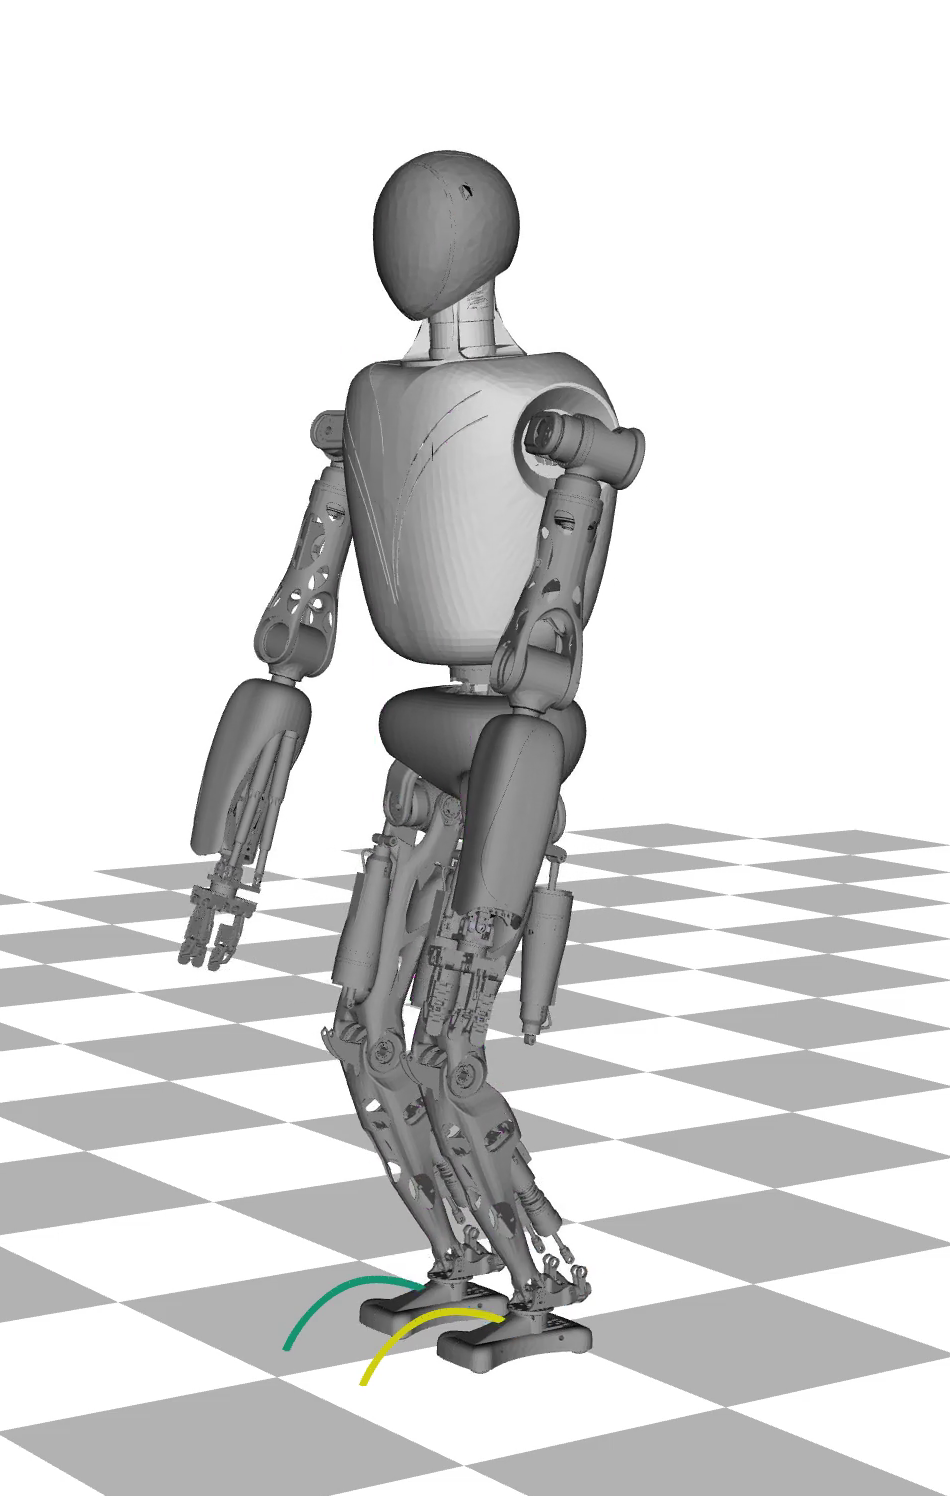
\includegraphics[width=1\linewidth]{fig/jumpForward/snaps/3x}
	\caption{}
	\end{subfigure}%
\begin{subfigure}{.16\textwidth}
	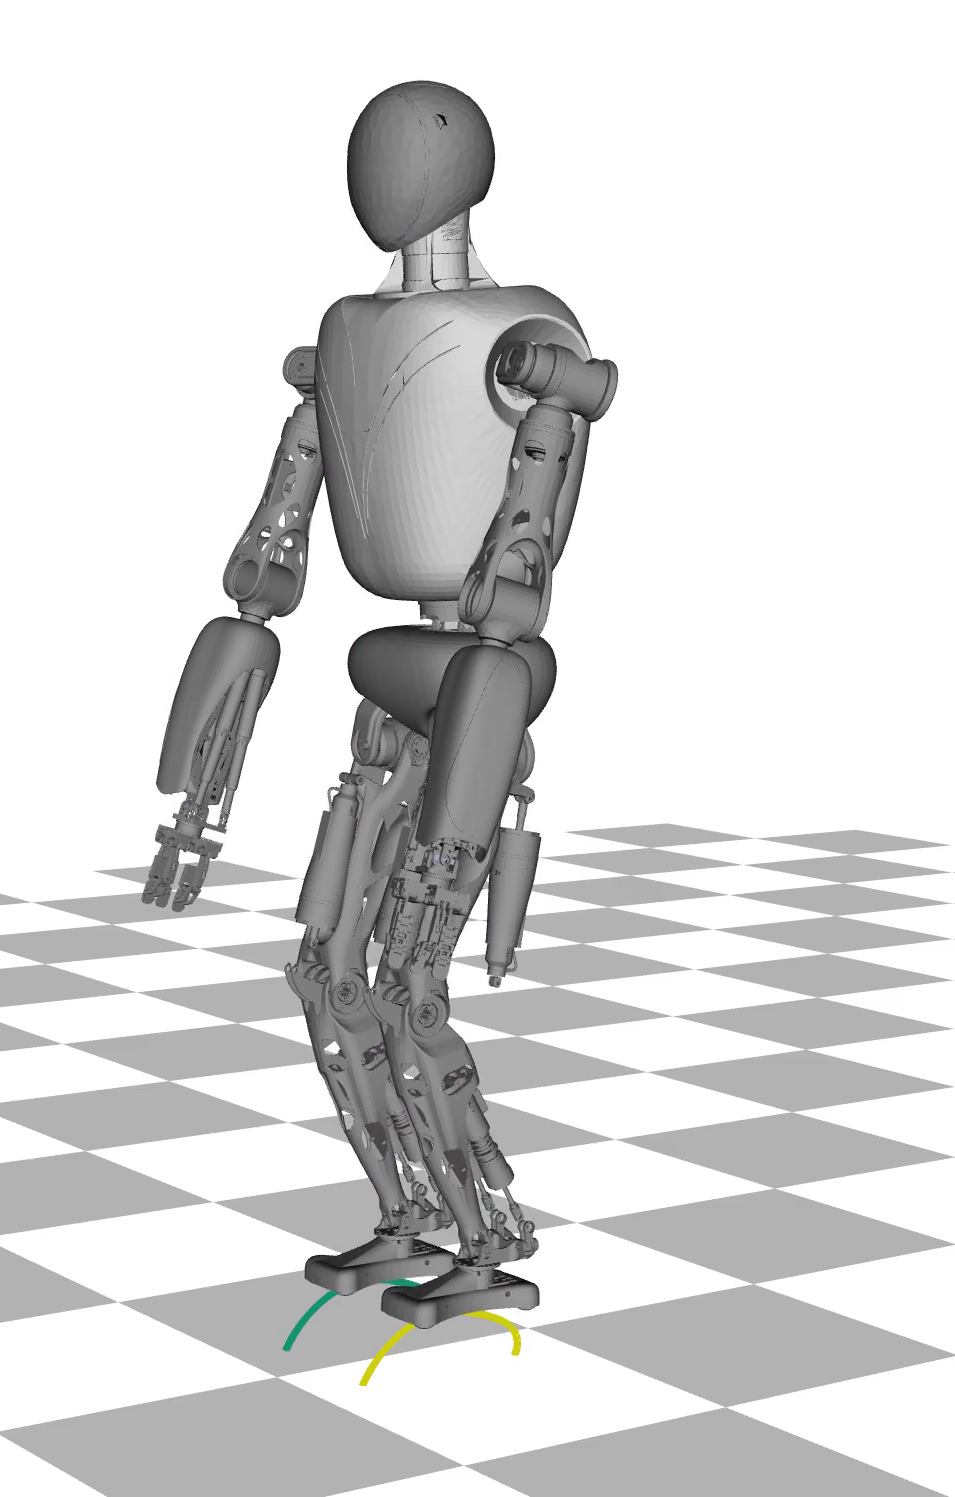
\includegraphics[width=1\linewidth]{fig/jumpForward/snaps/4x}
	\caption{}
\end{subfigure}%
\begin{subfigure}{.16\textwidth}
	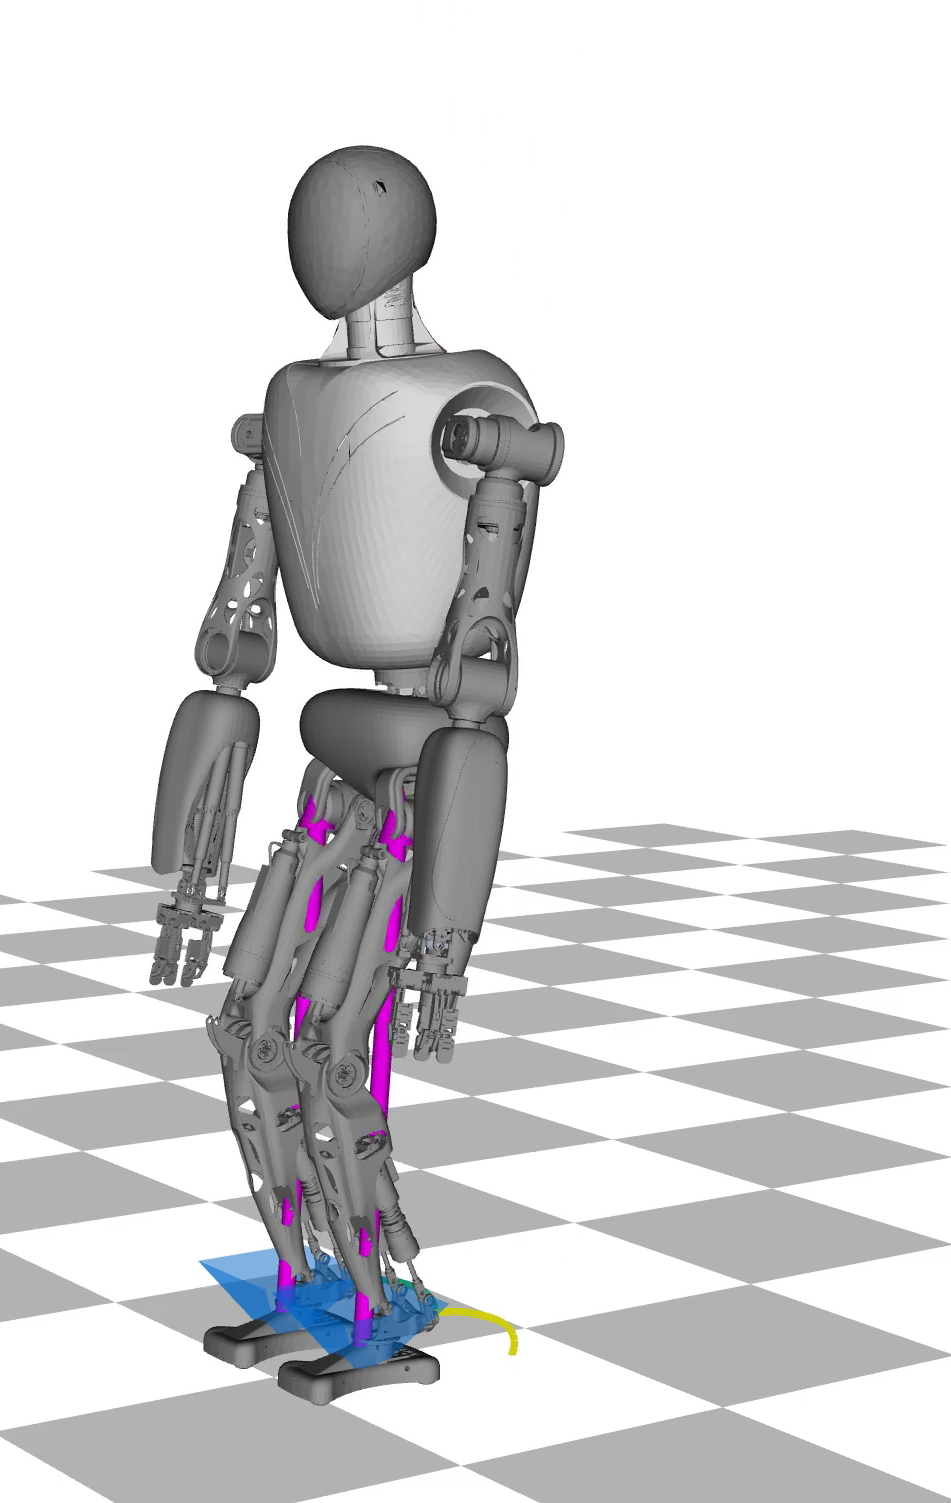
\includegraphics[width=1\linewidth]{fig/jumpForward/snaps/5x}
	\caption{}
	\end{subfigure}%
\begin{subfigure}{.16\textwidth}
	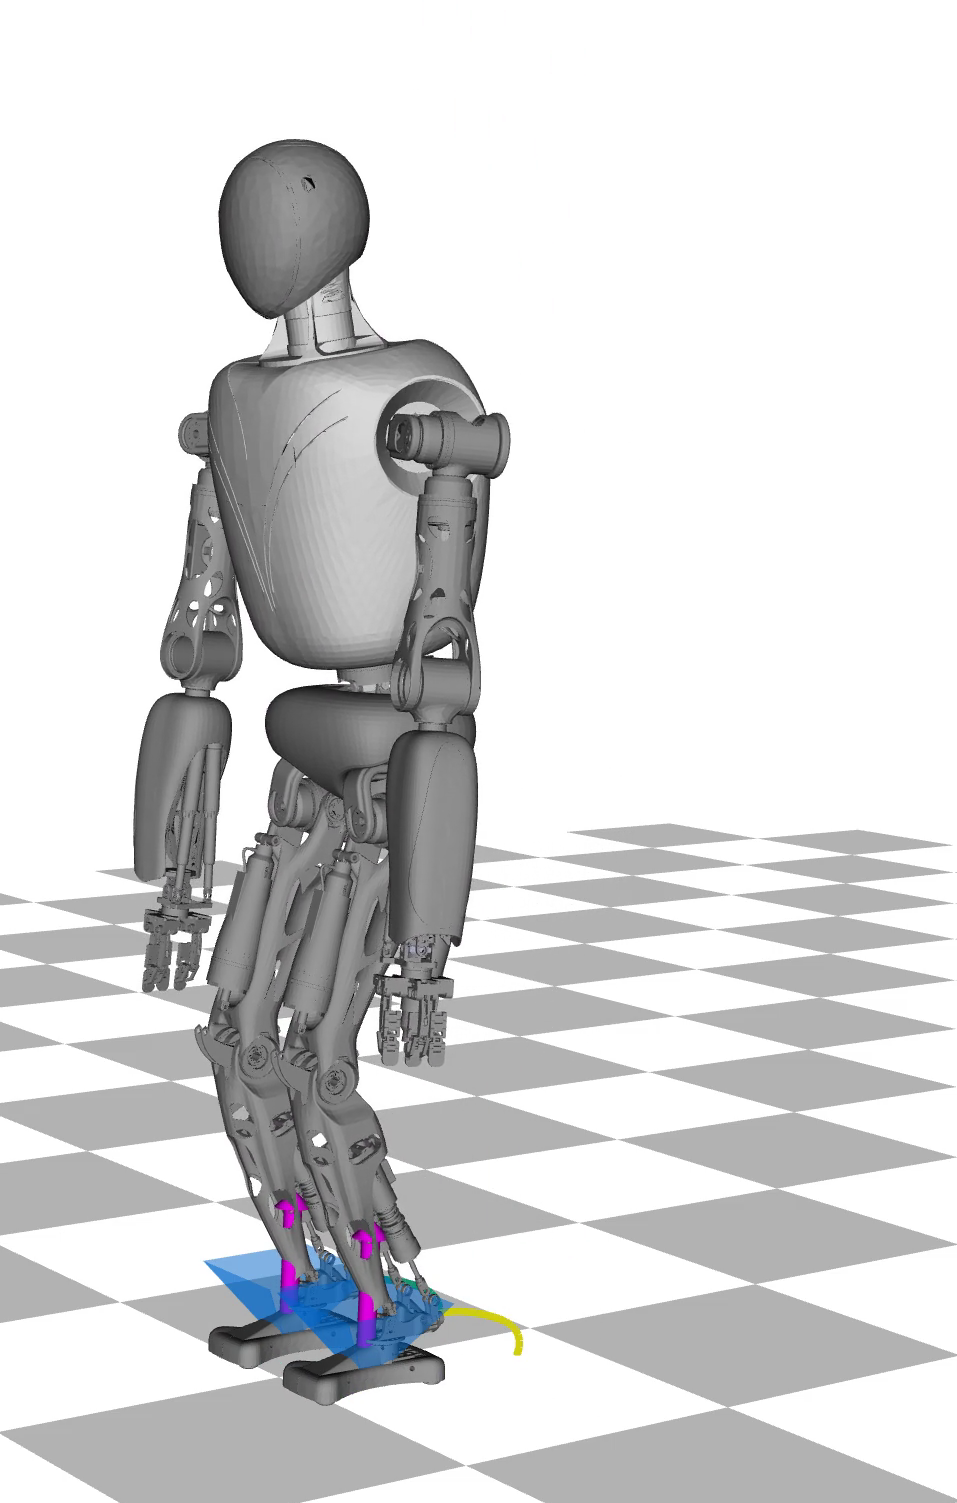
\includegraphics[width=1\linewidth]{fig/jumpForward/snaps/6x}
	\caption{}
\end{subfigure}%
\caption{A simple forward jump.}
\label{fig:jumpForward_Snaps}
\end{figure} 

\cref{fig:jumpForward_ContactWrenches} presents an overview about the solved optimal contact wrenches. When the robot does not move, the sum of vertical forces $F_z$ for left and right foot equals the body's weight, which is about 600 N. It becomes evident that about 4000 N (7 x robot weight) are exerted to the ground at lift off and about 8000 N (14 x robot weight) at touchdown, which is reasonable according to biomechanical findings \cite{meghdari2002dynamical}.
\begin{figure}[h!]
\centering	
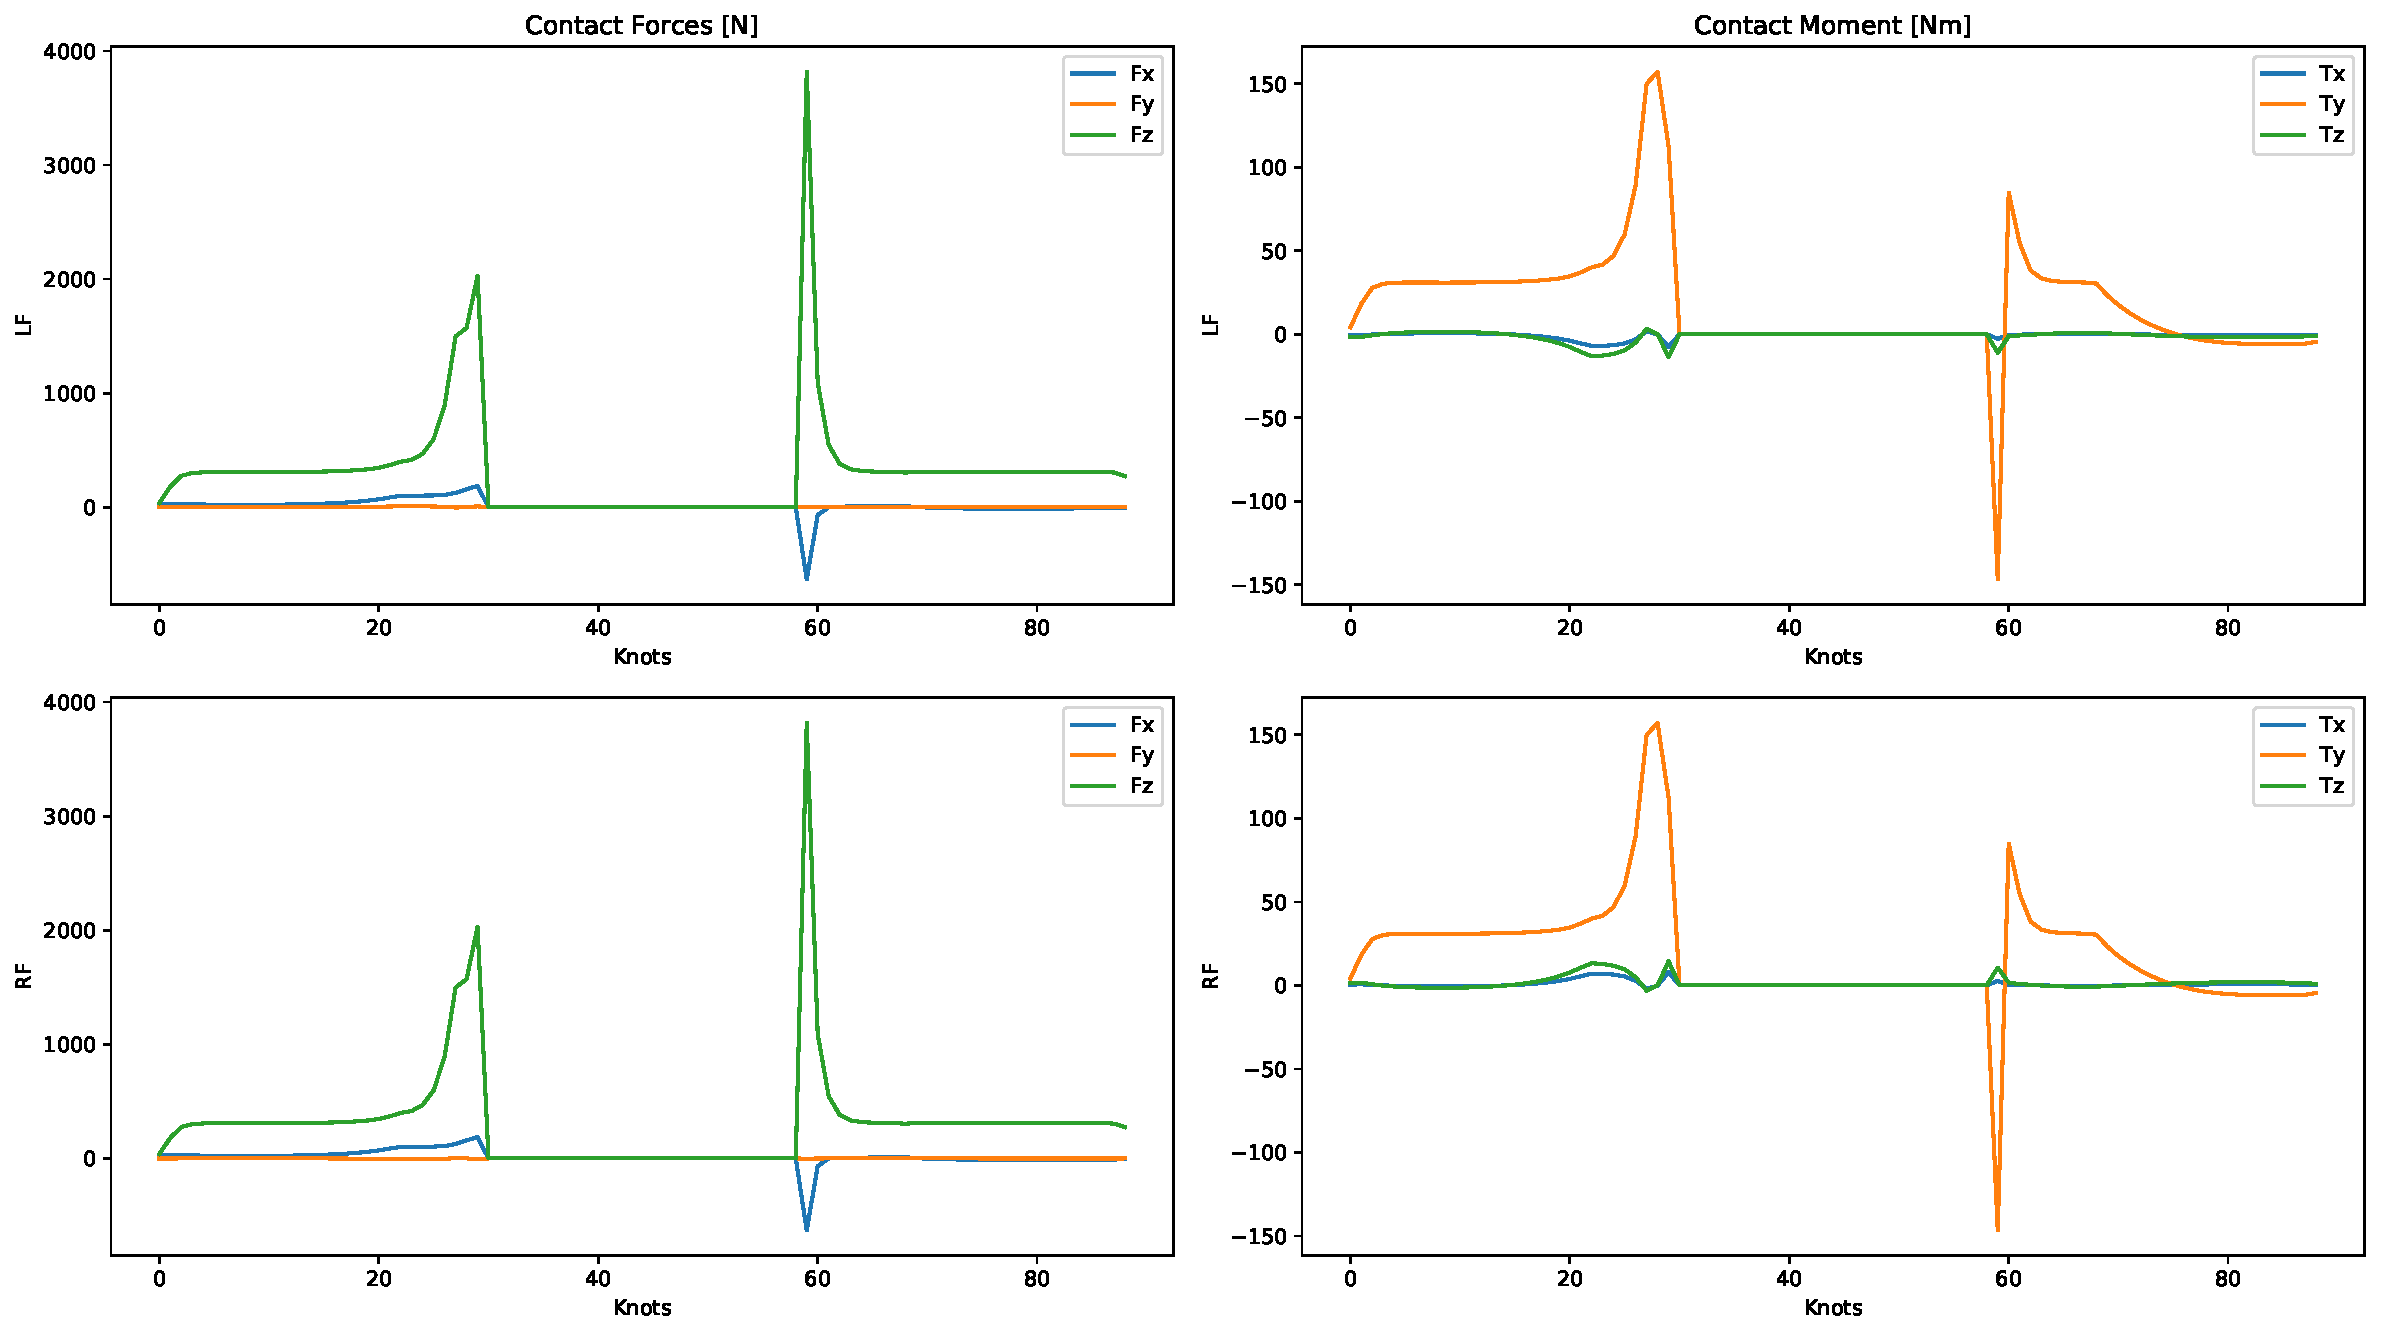
\includegraphics[width=1\textwidth]{fig/jumpForward/ContactWrenches}
\caption{Forward jump solution of the contact wrenches.}
\label{fig:jumpForward_ContactWrenches}
\end{figure} 

We have shown in \cref{sec:BipedEvaluation} that the proposed motion planning approach allows computation of dynamically balanced walking gaits. In the following, we want to investigate the feasibility of contact stability for highly-dynamic movements. \cref{fig:jumpForward_StabilityAnalysis} shows the stability analysis for the forward jumping task. It becomes clear that the \gls{CoP}s lie within the desired contact area of the left and right foot, respectively. Moreover, it can be observed that \gls{CoP}s are located more in the rear area of the sole of the foot before the jump or in the front area after landing. The first effect can be explained due to the angular momentum gained during descending of the base. The latter observation accounts for the rapid deceleration of the base motion in x-direction resulting from the instantaneous impact after the flight phase.    
\begin{figure}[h!]
\centering	
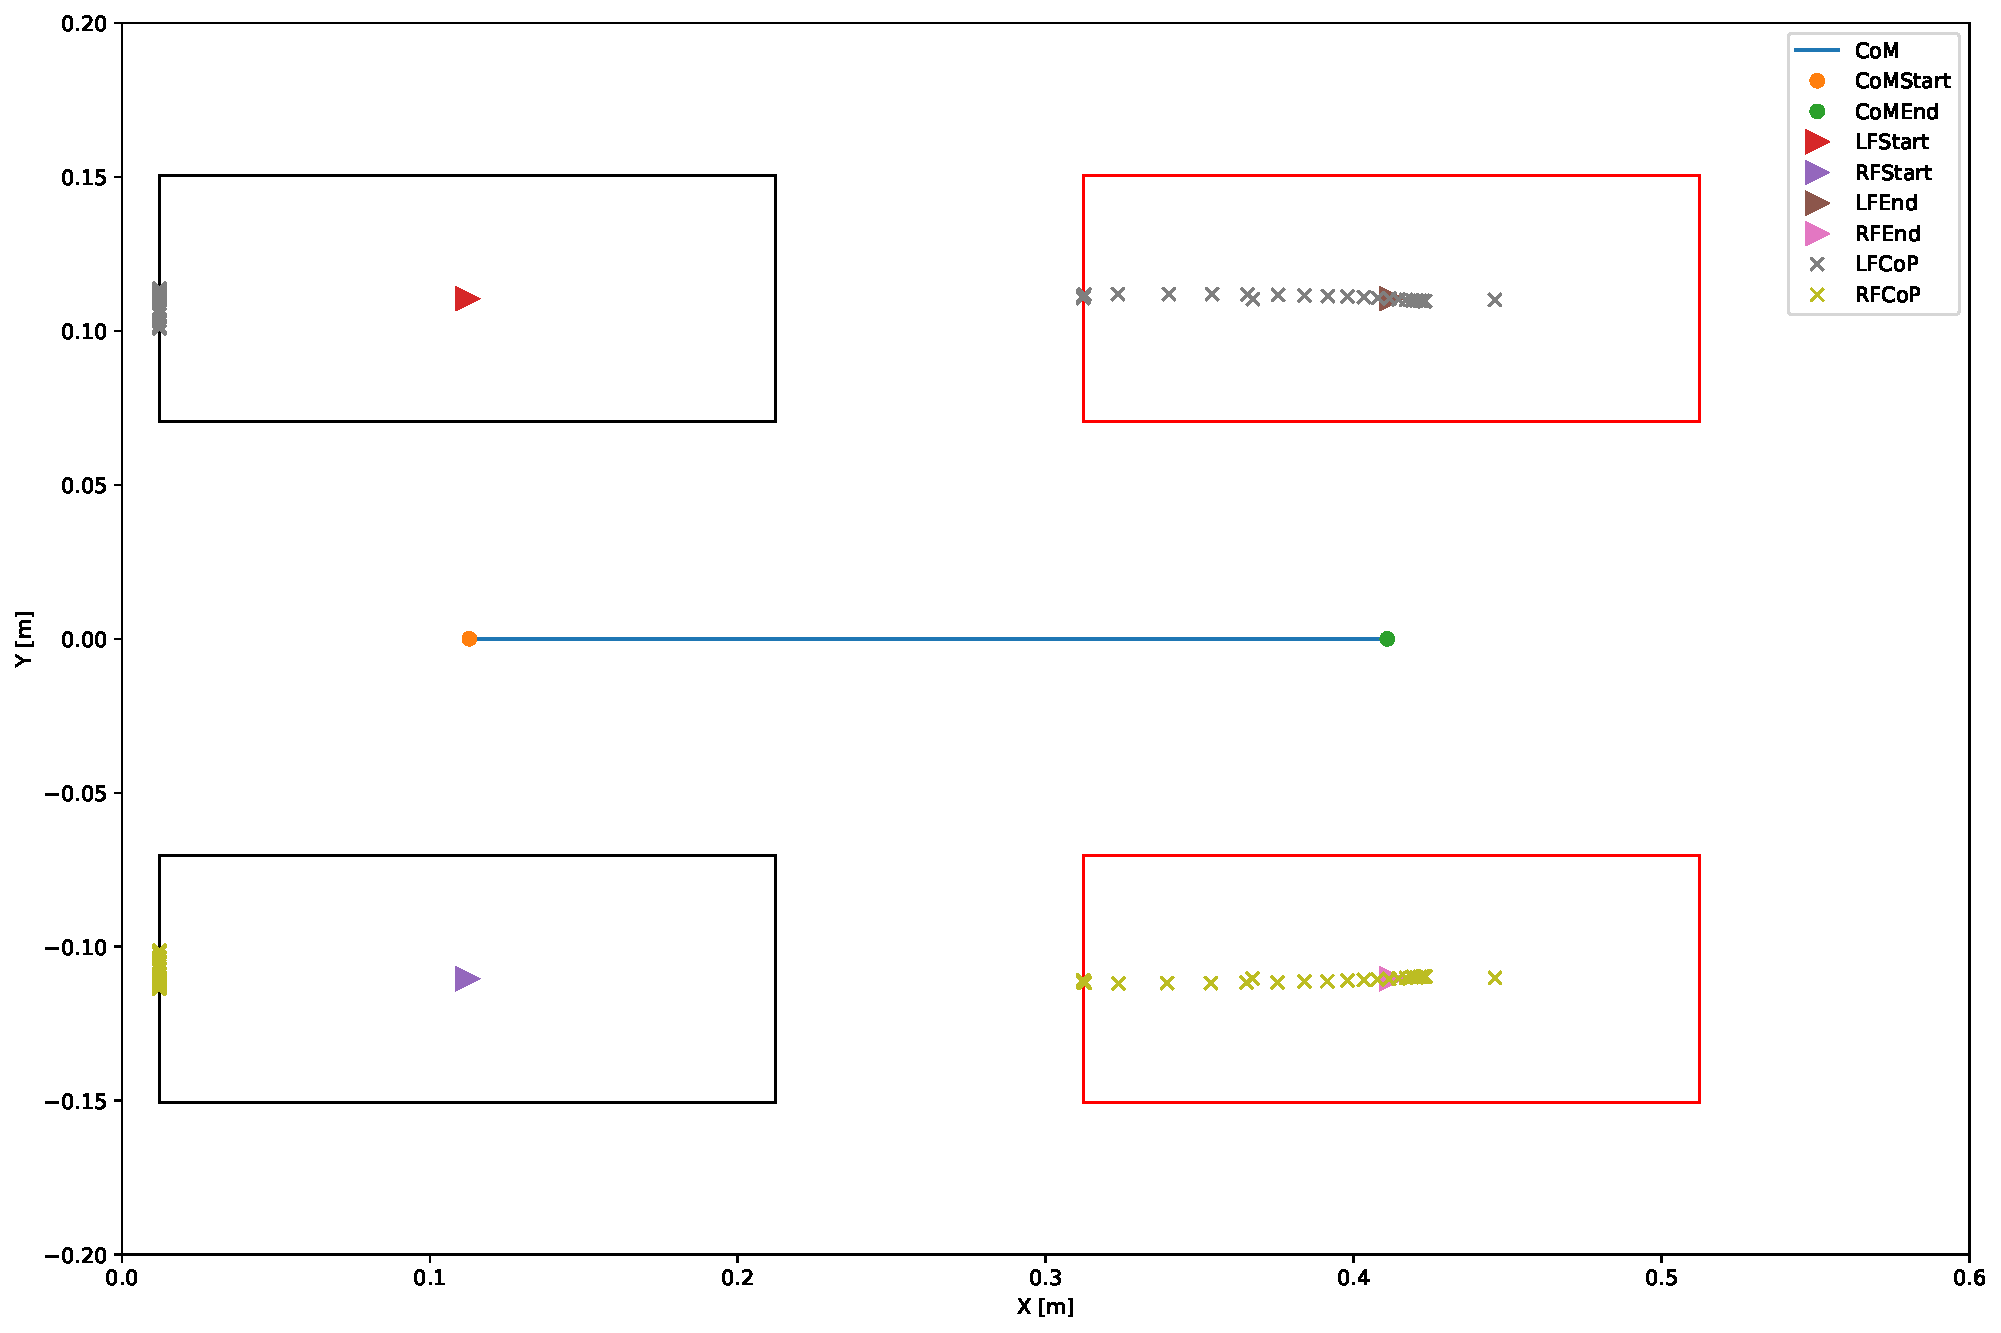
\includegraphics[width=.7\textwidth]{fig/jumpForward/StabilityAnalysis}
\caption{Stability analysis of the simple forward jump.}
\label{fig:jumpForward_StabilityAnalysis}
\end{figure} 

\subsection{Forward Jumping Over Multiple Obstacles}
Finally, we want to further increase the task dynamics and investigate the proposed motion planning approach for a challenging sequence of multiple forward jumps over obstacles. 

We build a sequence of \gls{OC} problems, as introduced in \cref{eqn:optimizationProblemSequence}, consisting of multiple forward jumps with increased jumping height and length (see \cref{tab:jumpObstacles}, accordingly. Since the RH5 humanoid was not designed for tasks of this dynamics, neither joint nor torque limits can be satisfied. In contrast to the simple vertical and forward jumps, this case study is supposed to proof the flexibility of the proposed motion planning approach rather than analyzing the system design. 

\begin{table}[t]
\centering
\caption{Multiple obstacles jumping characteristics and applied optimization constraints.}
\begin{tabular}{|ll|ll|}
\hline
\multicolumn{2}{|l|}{\textbf{Jump Characteristics}} & \multicolumn{2}{l|}{\textbf{Optimization Constraints}} \\ \hline
Number of jumps: & 3 	& Tasks: 			& Foot ($\Phi_1$) \\ \hline
Jump length:& 60 cm 	& Stability: 		& \gls{CoP} ($\Phi_3$), Friction Cone ($\Phi_4$)\\ \hline
Jump height:& 25 cm  	& Limits:   & / \\ \hline
Total time:& 1.2 s / jump  & Regularization: 	& Posture ($\Phi_7$), Torque ($\Phi_8$)\\ \hline
Step size:& 0.01 s & & \\ \hline
\end{tabular}
\label{tab:jumpObstacles}
\end{table}

\begin{figure}[h!]
\centering
\begin{subfigure}{.33\textwidth}
	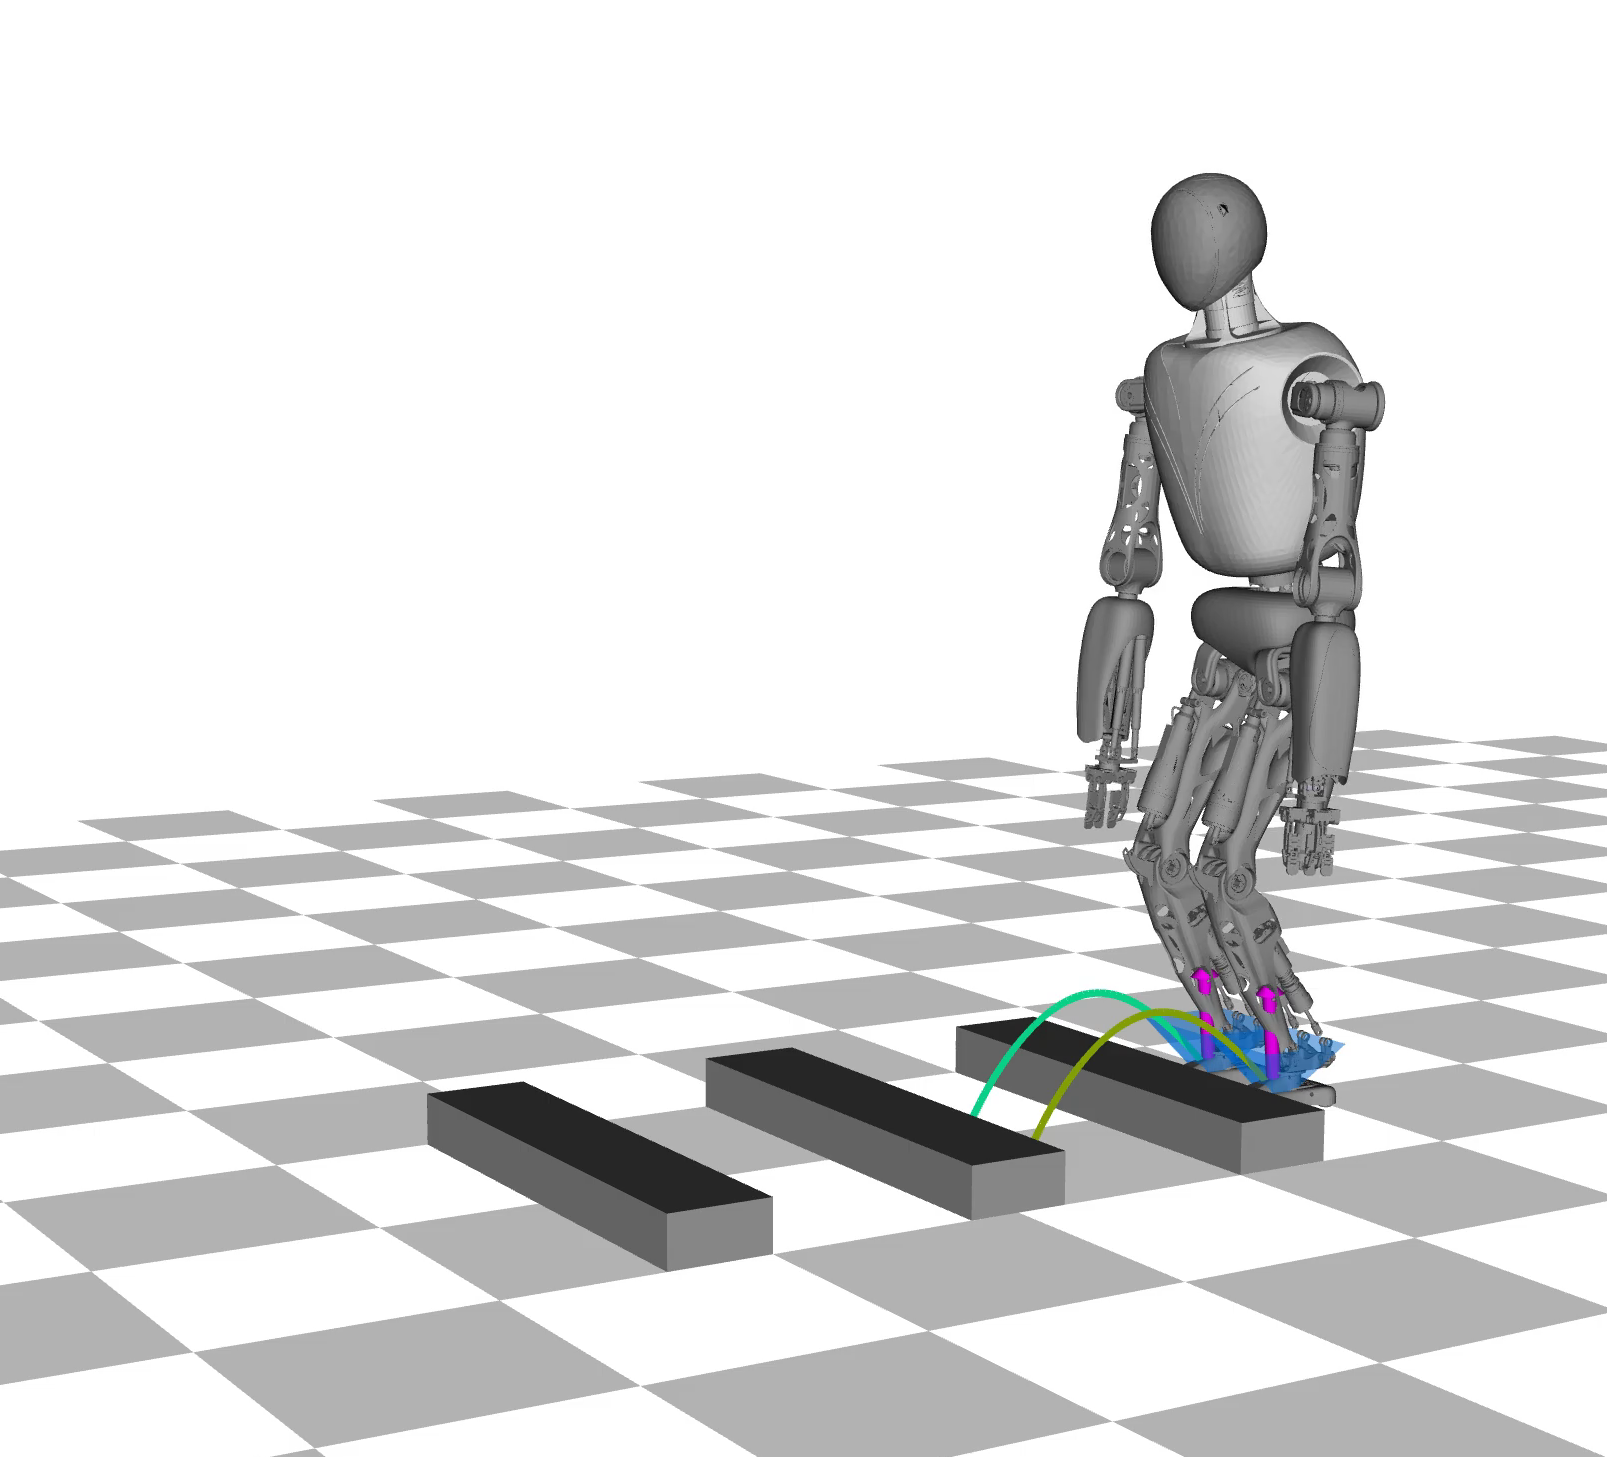
\includegraphics[width=1\linewidth]{fig/jumpObstacles/snaps/1x}
	\end{subfigure}%
\begin{subfigure}{.33\textwidth}
	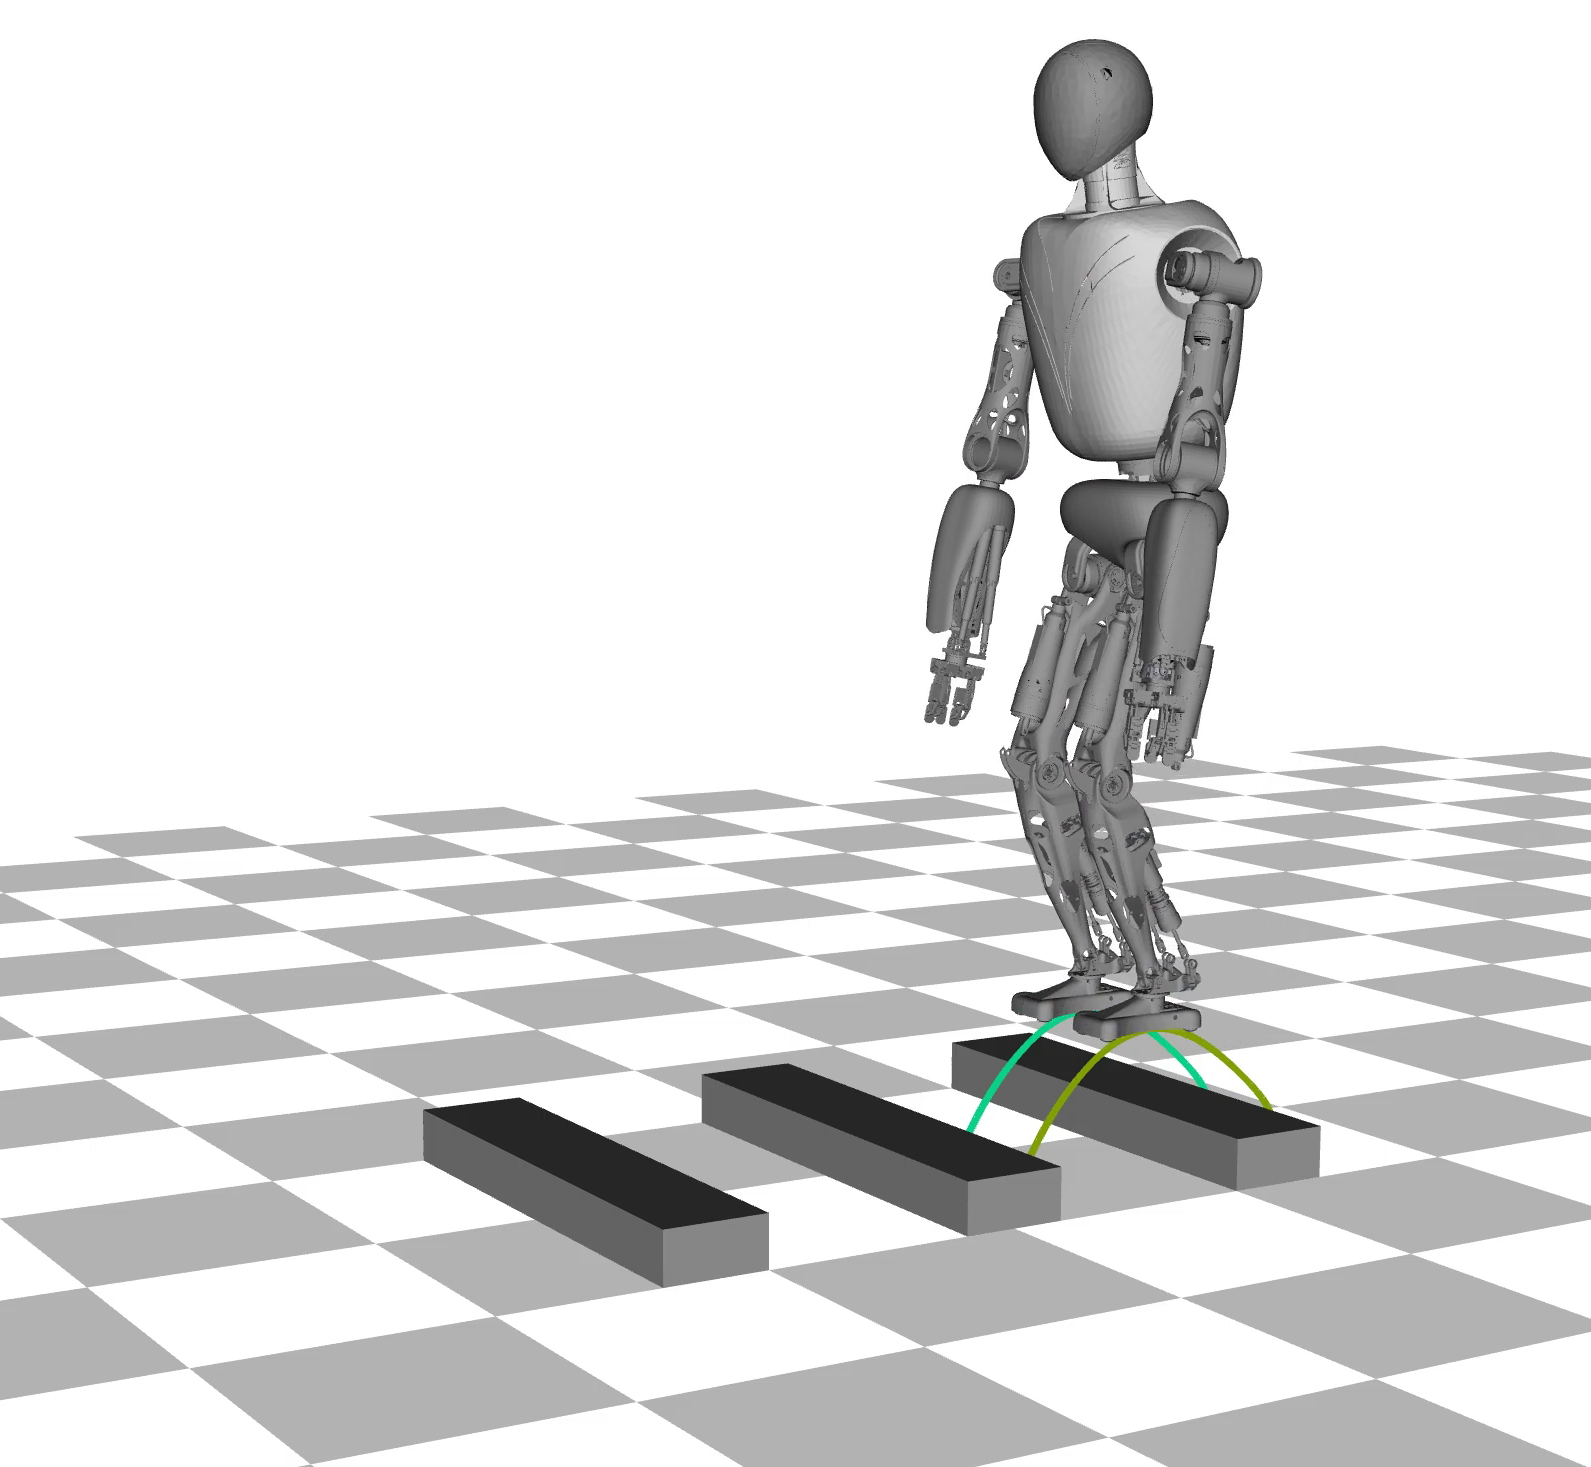
\includegraphics[width=1\linewidth]{fig/jumpObstacles/snaps/2x}
\end{subfigure}%
\begin{subfigure}{.33\textwidth}
	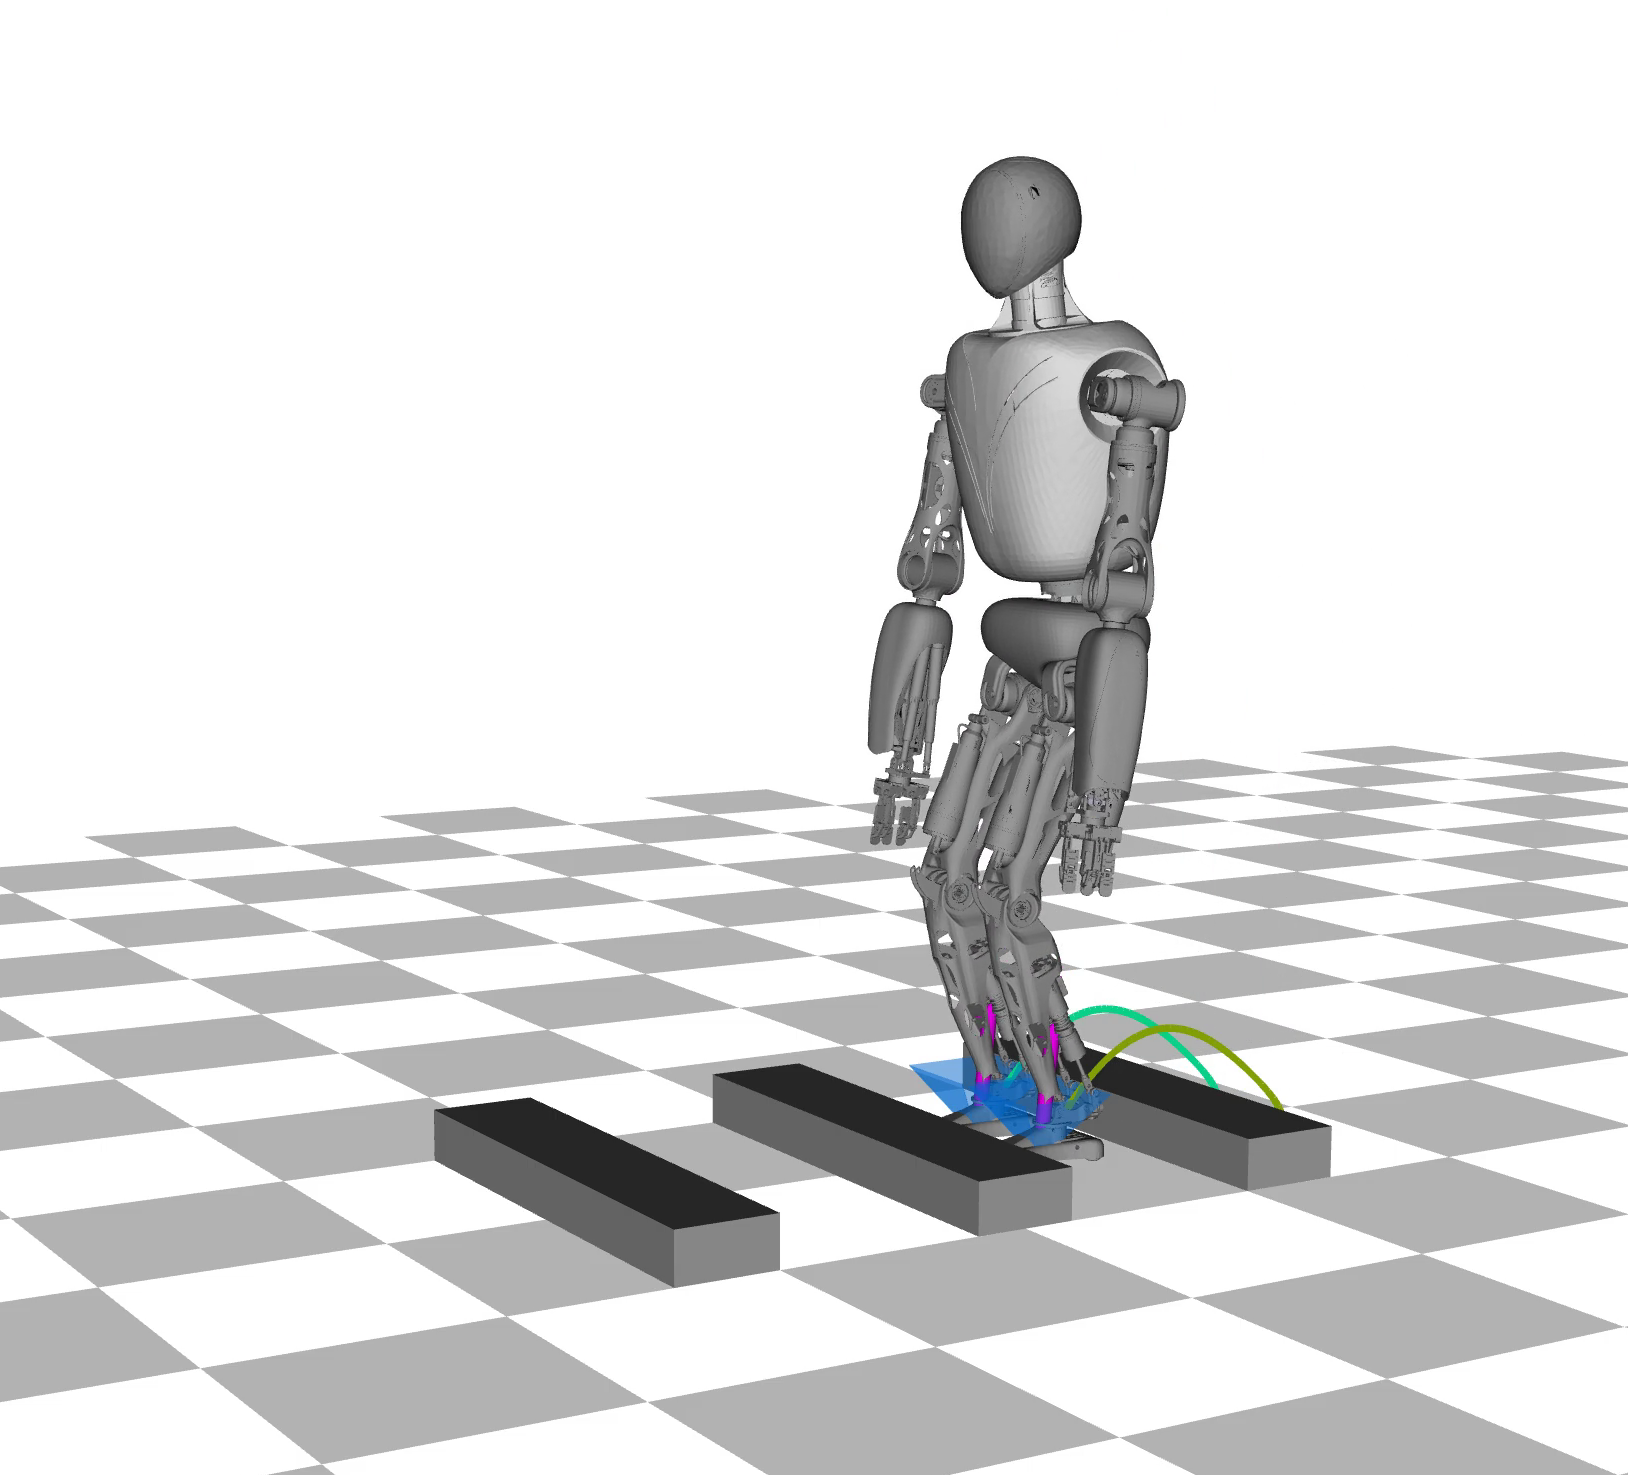
\includegraphics[width=1\linewidth]{fig/jumpObstacles/snaps/3x}
\end{subfigure}%
	
\begin{subfigure}{.33\textwidth}
	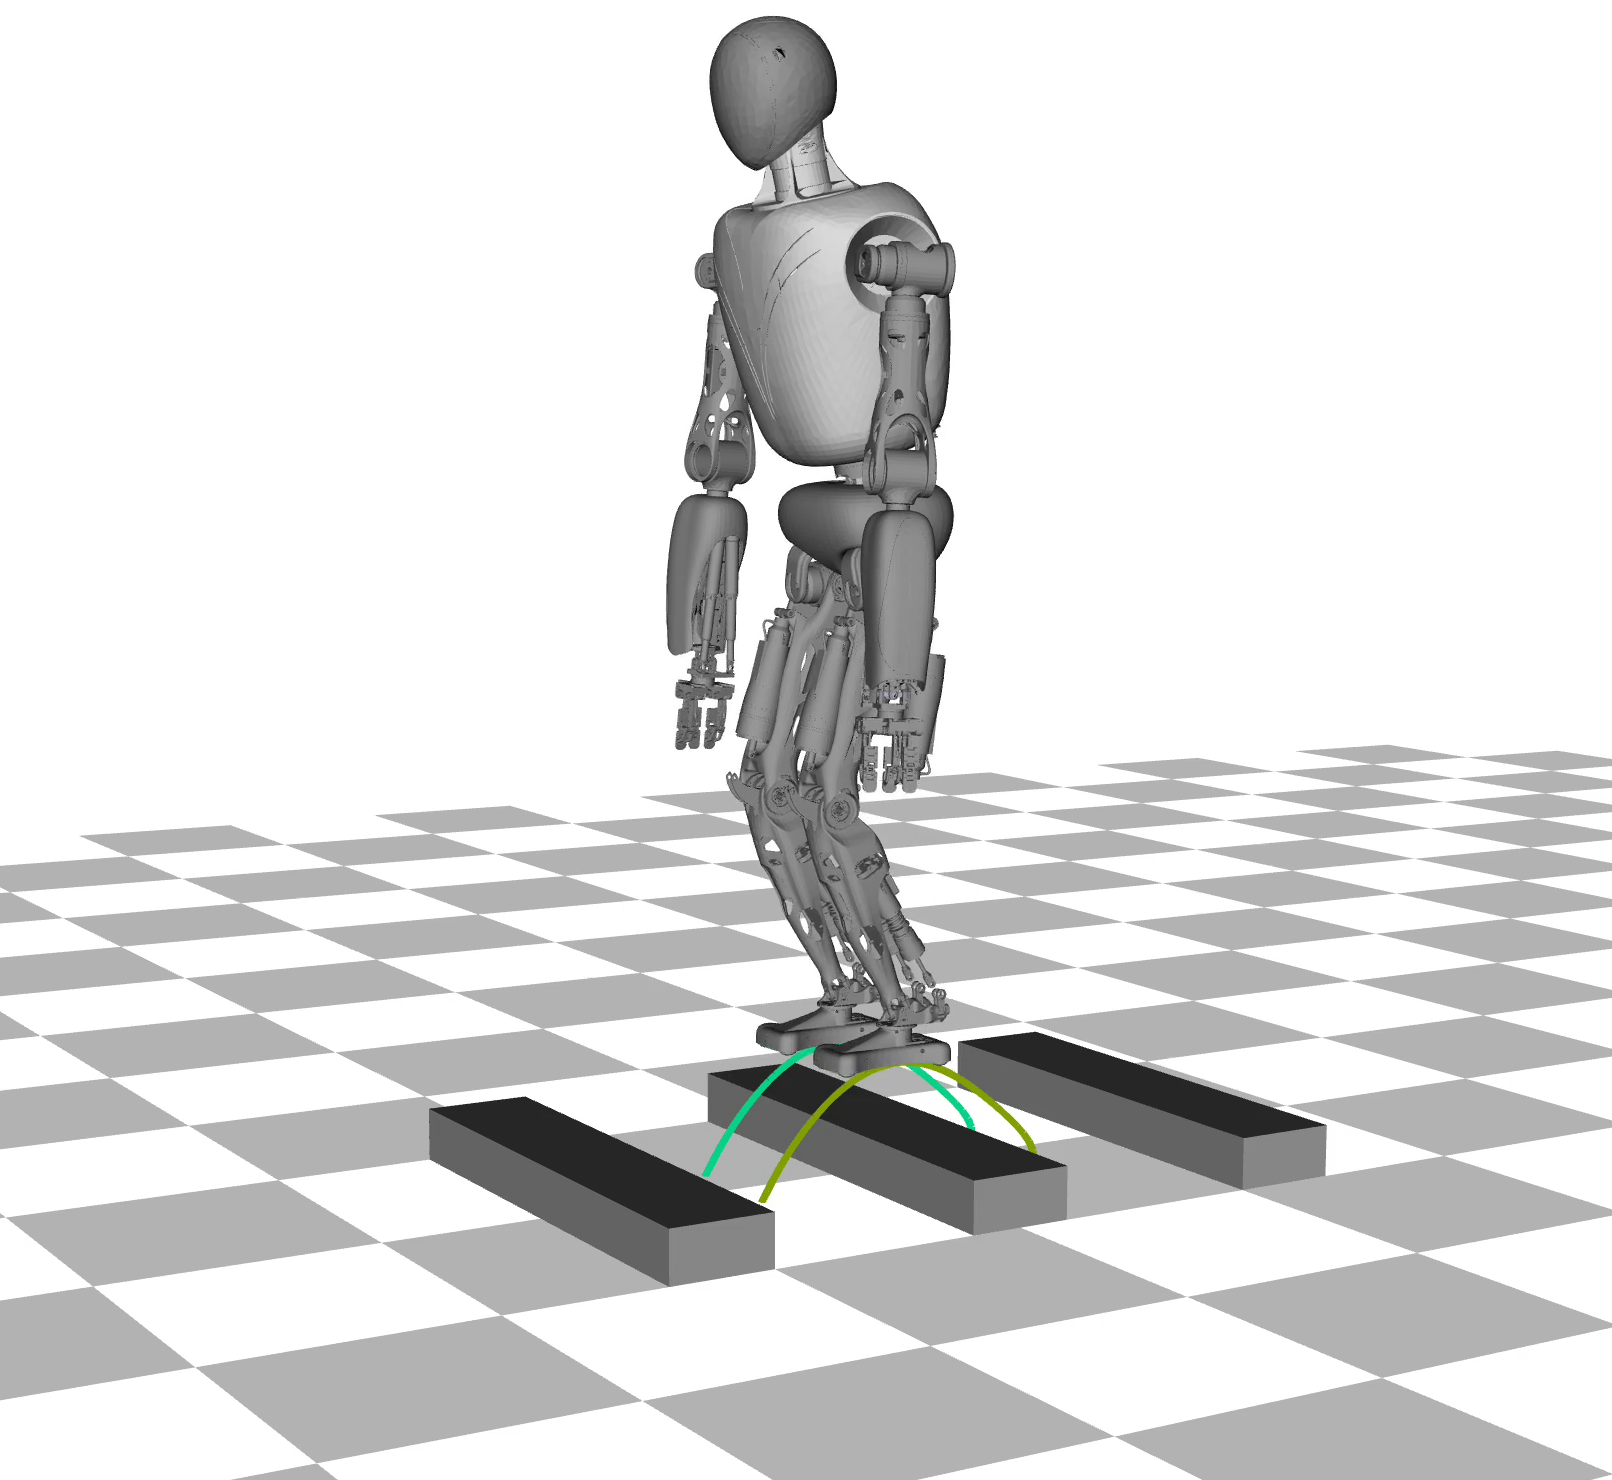
\includegraphics[width=1\linewidth]{fig/jumpObstacles/snaps/4x}
	\end{subfigure}%
\begin{subfigure}{.33\textwidth}
	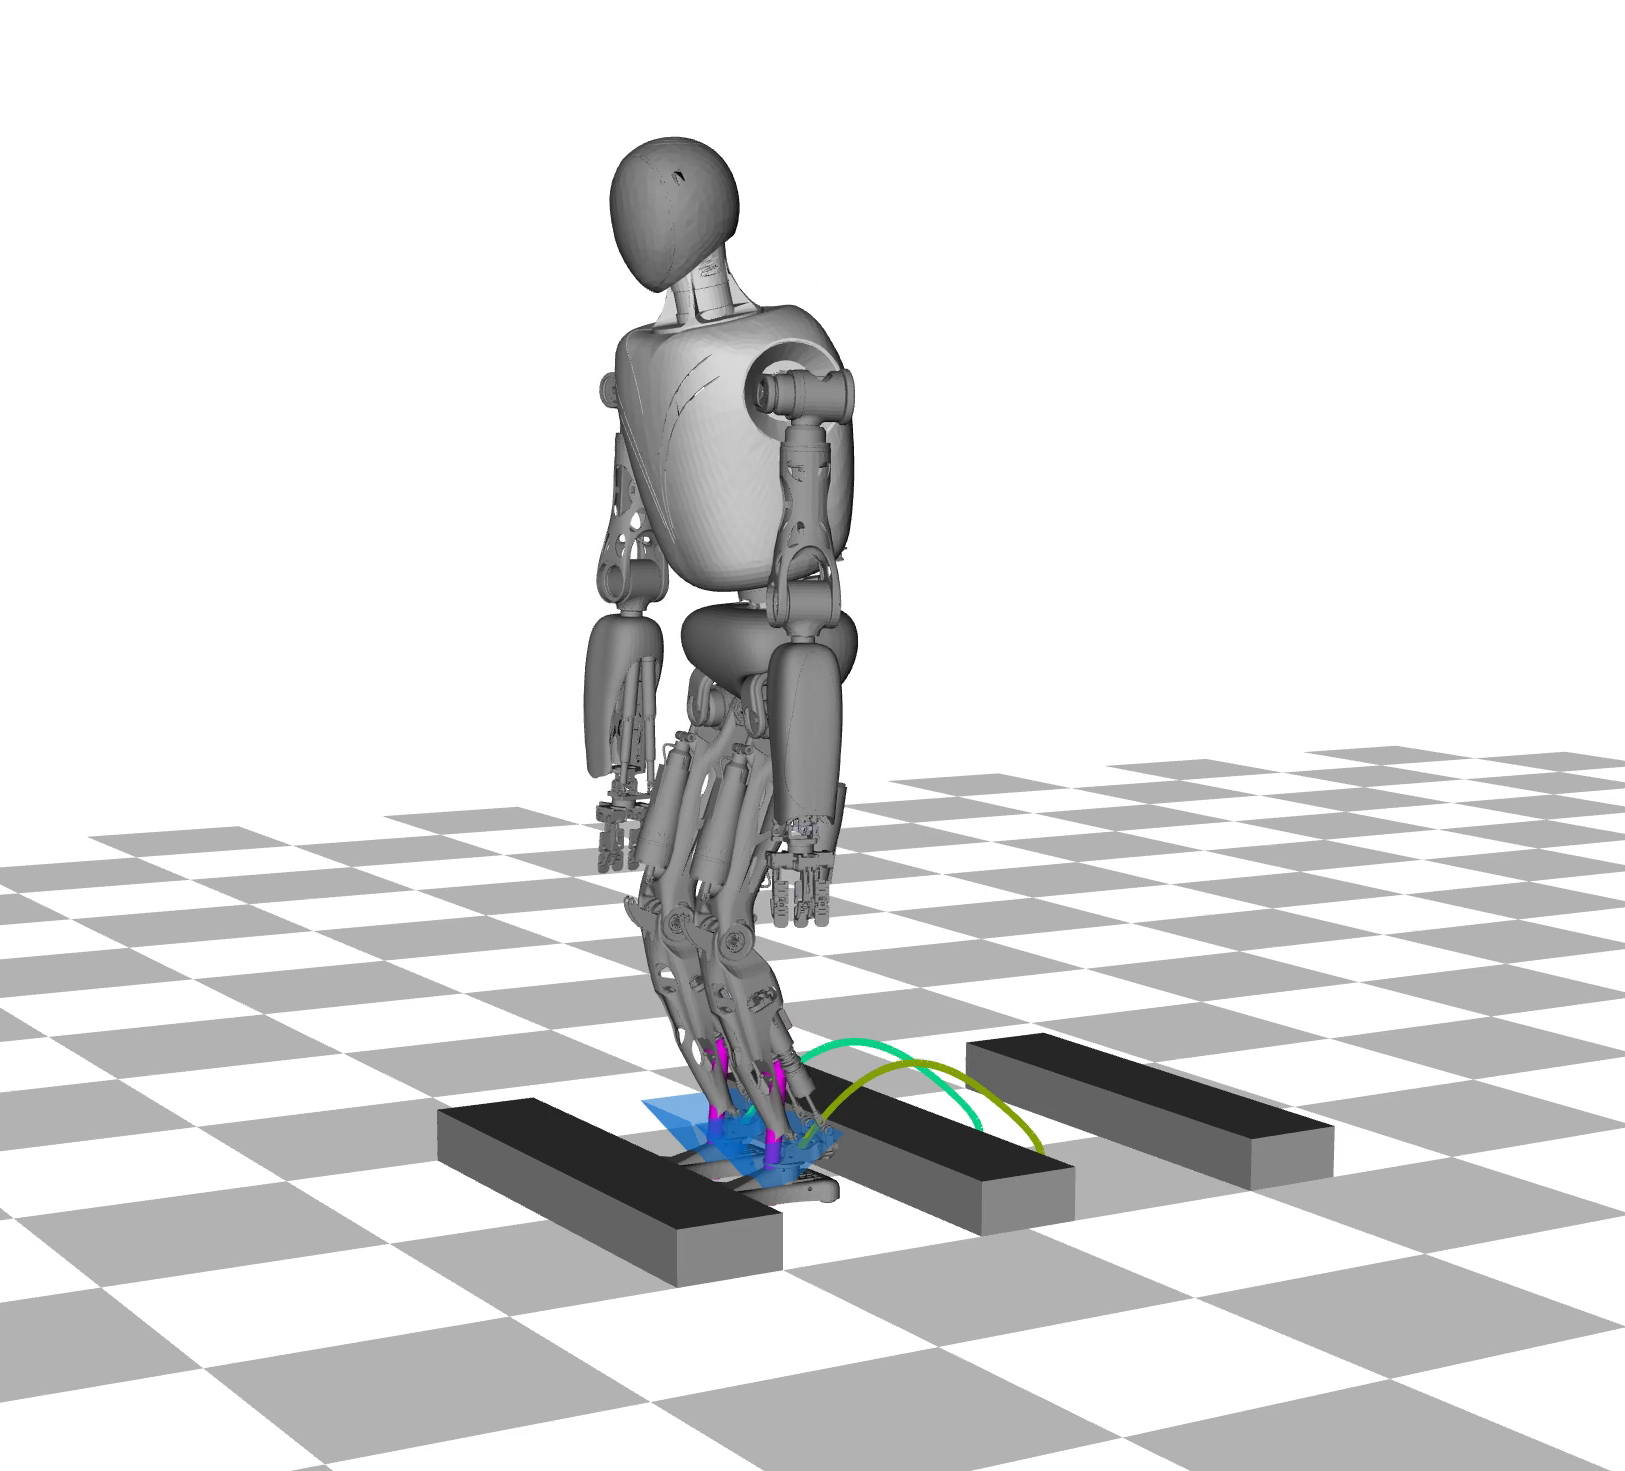
\includegraphics[width=1\linewidth]{fig/jumpObstacles/snaps/5x}
\end{subfigure}%
\begin{subfigure}{.33\textwidth}
	\includegraphics[width=1\linewidth]{fig/jumpObstacles/snaps/6x}
\end{subfigure}%

\begin{subfigure}{.33\textwidth}
	\includegraphics[width=1\linewidth]{fig/jumpObstacles/snaps/7x}
\end{subfigure}%

\caption{Multi-phase \gls{OC} problem of forward jumping over obstacles. Image order: column-wise, from top to bottom and left to right.}
\label{fig:jumpObstacles_Snaps}
\end{figure} 

Previously, we have demonstrated that the contact stability constrained \gls{DDP} allows computation of a simple forward jump with dynamical balanced motions. Following up, we want to study if the concept also holds for multiple forward jumps. 

\cref{fig:jumpObstacles_StabilityAnalysis} shows the obtained results for stability analysis for sequentially solving the sequence of optimization problems. The robot starts in an initial pose in \gls{DS}, performs a jump and recovers to the intial pose again. This \gls{OC} problem is repeated for three times with identical constraints and timings until the robot reaches the final \gls{DS} pose marked by red rectangles. As becomes evident, the contact stability constrained \gls{DDP} forces the \gls{CoP}s of both feet to lie within the desired contact area proofing for dynamically balanced motions. 

\begin{figure}[h!]
\centering	
\includegraphics[width=1\textwidth]{fig/jumpObstacles/StabilityAnalysis}
\caption{Stability analysis of forward jumping over multiple obstacle.}
\label{fig:jumpObstacles_StabilityAnalysis}
\end{figure}

Recapitulating the results for the simple forward jump, we identified that the \gls{CoP}s are located in the rear area of the foot sole during takeoff. We can draw similar conclusions for the first jump of the multi-phase \gls{OC} problem. However, the \gls{CoP}s for the second and third jump do not share this pattern. This effect can be attributed to the dynamic forces already acting on the robot while the second and second impact phase, respectively.


%\section{Identification of Limits in System Design}
%\section{Evaluation of the System Design}
%
%This section presents an exhaustive study of the system limits of the RH5 humanoid robot based on the case studies introduced from the last section. The motivation is form a basis of decision-making for future design iterations to perform highly-dynamic movements with the humanoid in real-world experiments.
%
%\begin{table}[t]
%\centering
%\caption{Capabilities of the RH5 humanoid to perform highly-dynamic motions.}
%\begin{tabular}{lccc}
%\hline
%& Motor Torque & Joint Position & Joint Velocity \\ \hline
%Vertical Jump & & & \\
%\quad\quad 1 cm 		& \greencheckmark  & \greencheckmark & \greencheckmark \\
%\quad\quad 5 cm 		& \greencheckmark  & \greencheckmark & \redxmark \\
%\quad\quad 10 cm 		& \greencheckmark  & \greencheckmark & \redxmark \\
%\quad\quad 20 cm 		& \greencheckmark  & \greencheckmark & \redxmark \\
%\quad\quad 30 cm 		& \greencheckmark  & \greencheckmark & \redxmark \\ \hline
%Forward Jump (h=10 cm)& & & \\
%\quad\quad 10 cm 		& \greencheckmark  & \greencheckmark & \redxmark \\
%\quad\quad 20 cm 		& \greencheckmark  & \greencheckmark & \redxmark \\
%\quad\quad 30 cm 		& \greencheckmark  & \greencheckmark & \redxmark \\
%\quad\quad 40 cm 		& \greencheckmark  & \greencheckmark & \redxmark \\
%\quad\quad 50 cm 		& \greencheckmark  & \greencheckmark & \redxmark \\ \hline
%Obstacle Jump (h=25 cm)& & & \\
%\quad\quad 60cm 		& \redxmark  & \redxmark & \redxmark \\ \hline
%
%\end{tabular}
%\label{tab:systemLimits}
%\end{table}






































 





\chapter{Introduction}\label{c1}
\section{Motivation}
\section{Related Work}
%\subsection{Model Induced Design} (Passive Dynamic Walking, Template Models)
%\subsection{Traditional Legged Locomotion Planning}
%\subsection{Trajectory Optimization} (Sequential, Simultaneous OR Direct, Indirect, DDP)
%\subsection{Series-Parallel Hybrid Robots}
\section{Contribution}
\section{Structure}

%-----------------------------------------------------------------------------%
%                                                                             %
%    K A P I T E L   2                                                        %
%                                                                             %
%-----------------------------------------------------------------------------%

\chapter{Mathematical Background: Optimal Bipedal Locomotion}\label{c2}
The second chapter provides the reader with fundamentals regarding terminology, modeling and stability analysis in the context of humanoid robotics and presents the class of used algorithms with its relevant extensions used in the context of this thesis.

\section{Foundations of Bipedal Locomotion}\label{sec:TheoryBiped}
\subsection{Terminology}
In order to describe the locomotion of a humanoid robot, specific terms are required that are introduced within this section. \citeauthor{vukobratovic2007towards} provide an extensive introduction to the terminology related to bipedal walking \cite{vukobratovic2007towards}, concisely summarized by \citeauthor{dekker2009zero} \cite{dekker2009zero}.\\\\
\textbf{Walk}\\
Walk can be defined as: ``\textit{Movement by putting forward each foot in turn, not having both feet off the ground at once}''.\\\\
\textbf{Run}\\
Run in turn is characterized by  a movement where partially both feet leaving the ground at the same time.\\\\
\textbf{Gait}\\
The way each human walks and runs is unique, hence gait can be defined as: ``\textit{Manner of walking or running}''.\\\\
\textbf{Periodic gait}\\
If a gait is realized by repeating each locomotion phase in an identical 
\footnote{The locomotion phase can be identical w.r.t. the step size or the duration, depending on the index.} way, the gait is referred to as \textit{periodic}.\\\\
\textbf{Symmetric gait}\\
If the left and right leg move in an identical but time-shifted manner, the gait is referred to as \textit{symmetric}.\\\\
\textbf{Double Support}\\
A situation where the humanoid has two isolated contact surfaces with the ground.\\\\
\textbf{Single Support}\\
A situation where  the humanoid has only one contact surface with the ground.\\\\
\textbf{Support Polygon}\\%TODO: Maybe add figure to illustrate single vs double support
The support polygon is formed by the \textit{convex hull} about the ground contact points.    \\\\
\textbf{Swing foot}\\
This term refers to the leg that is performing a step, i.e. moving through the air.\\\\
\textbf{Supporting foot}\\
This term refers to the leg that is in contact with the ground, supporting all the weight of the humanoid. 

\subsection{Dynamic Modeling of Legged Robots}\label{subsec:DynamicModeling}
In the following, the dynamic model for floating base systems, such as legged robots, is derived based on a general formulation. A concise introduction to dynamic modeling is presented with \cite{scaronTeaching}, comprehensive studies can be found in \cite{pfeiffer1996multibody, jain2010robot, featherstone2014rigid}.
\subsubsection{General Formulation}
Mathematical models of a robot's dynamics describe the motion as a function of time and control inputs. These models are the basis for both simulation and control of robotic systems. In an abstract form, the \gls{EoM} can be written as: 
\begin{equation} \label{eqn:EoMGeneral}
F(\bq(t),\bdq(t),\bddq(t),\bu(t),t)=0,
\end{equation}
where 
\begin{itemize}
\item \myM{t} is the time variable, 
\item \myM{q} is the vector of generalized coordinates,
\item $\bdq$ is the first time derivative (velocity) of \myM{q}, 
\item $\bddq$ is the second time derivative (acceleration) of \myM{q} and
\item \myM{u} is the vector of control inputs. 
\end{itemize}
Consequently, the \gls{EoM} provide a mapping between the control space on the one hand and the state space of robot on the other hand. Typical methods for computing the closed-form solution of the \gls{EoM} are e.g. the classical \textit{Newton-Euler} \cite{luh1980line} method or the \textit{Lagrange method} \cite{hollerbach1980recursive}, where the former is based on principles for conservation of linear and angular momenta and the latter utilizes energy-based functions expressed in generalized coordinates. 
\subsubsection{Fixed Base Systems}
For applications with fixed-based robots, e.g. a robotic manipulator, the multi-body dynamics can be formulated as
\begin{equation} \label{eqn:EoMManipulator}
\myM{M}(\bq)\bddq+\bdq^T\myM{C}(\bq)\bdq=\btau+\btau_g(\bq),
\end{equation}
where 
\begin{itemize}
\item $\myM{M}(\bq)$ is the generalized inertia matrix, 
\item $\myM{C}(\bq)$ is the coriolis tensor, 
\item $\btau$ is the vector of actuated joint torques and 
\item $\btau_g(\bq)$ is the vector of external joint torques caused by gravity.
\end{itemize}
In contrast to the general formulation in \cref{eqn:EoMGeneral}, this expression is time-invariant. Hence, \cref{eqn:EoMManipulator} can be used for computing the \gls{FD}, as well as the \gls{ID} of a robotic system.
\subsubsection{Floating Base Systems}
A floating base system is characterized by having a base that is free to move, rather than being fixed in space. Consequently, the vector of generalized coordinates $\bq$ not only contains the joints angles, but also accounts for the position and orientation of the floating base. Legged robots belong to this category of rigid-body systems as they make and break contacts with their environment in order to move. Contrary to manipulators, contacts need to be actively enforced by holonomic constraints for legged robots. There are namely two different types of contact constraints that can be applied: point contacts (3d) or surface contacts (6d). 

For the case of point contacts, the dynamics of the floating base system become
\begin{equation*} \label{eqn:EoMLeggedRobotPtContact}
\myM{M}(\bq)\bddq+\bdq^T\myM{C}(\bq)\bdq=\myM{S}^T\btau+\btau_g(\bq)+\sum_{i=1}^{k}\myM{J}_{C_i}^T\myM{f}_i,
\end{equation*}
where 
\begin{itemize}
\item \myM{S} is the selection matrix of actuated joints,
\item $\myM{J}_{C_i}$ is the Jacobian at the location of a contact point $C_i$ and
\item $\bfun_i$ is the contact force acting at the contact point $C_i$.
\end{itemize}
For the case of surface contacts, such as a flat foot on a flat floor, modeling a point contact is not sufficient since it only constrains the translation. In order to also account for the rotational constraints enforced by the geometry one could take into account multiple point contacts. A non-redundant alternative is to model more general frame contact constraints as
\begin{equation} \label{eqn:EoMLeggedRobotSurfaceContact}
\myM{M}(\bq)\bddq+\bdq^T\myM{C}(\bq)\bdq=\myM{S}^T\btau+\btau_g(\bq)+\sum_{i=1}^{k}\myM{J}_{C_i}^T\myM{w}_i,
\end{equation}
where $\myM{w}_i$ is referred to as the \textit{contact wrench} acting on the contact link $i$. This wrench stacks the resultant $\bfun_i$ of contact forces and the moment $\btau_i$ exerted by these forces around the contact frame as
$$\myM{w}_i=(\myM{f}_i,\btau_i)_{6\times 1}.$$ 
For more details on contact wrenches and spatial vector algebra in general, the interested reader is referred to e.g. \cite[Ch.2]{featherstone2014rigid}.

%\subsection{Motion Generation}
%\subsection{Motion Control}
%\subsubsection{Kinematic Control (High-gain joint position trajectory tracking)}
%\subsubsection{Impedance Control with Joint Space Inverse Dynamics (Low-gain joint control with model compensation)}
%\subsubsection{Task Space Inverse Dynamics Control (Directly regulating in «task space»)}
%\subsubsection{Virtual Model Control (Dynamic control of a quasistatic system)}
%\subsection{Efficient Walking}


\section{Stability Analysis: Not Falling Down}\label{sec:TheoryStability}
Humanoid robots are high-dimensional, constrained and nonlinear dynamical systems. In this section, the most common criteria  for analyzing the long-term stability behavior of such complex systems are presented. Exhaustive studies on stability criteria and their relation can be found in \cite{garcia2002classification, dekker2009zero, siciliano2016springer}.

\subsection{Static Stability Criteria}
\subsubsection{Floor Projection of the Center of Mass (FCoM)}
Consider the case of a robot that is not moving, i.e. a humanoid in static double support. In that case, the only forces acting on the humanoid are the ones caused by gravity. These forces can be represented by a virtual force acting on the \gls{CoM} of the robot. The position of the \gls{CoM} w.r.t. the base frame can be described by
\begin{equation*} 
\bp_{CoM}=\dfrac{\sum_{i=1}^{n}m_i\bp_i}{\sum_{i=1}^{n}m_i},
\end{equation*}
where the robot has $n$ links and $\myM{p}_i$ indicate the according link distances of the individual \gls{CoM}s. The \gls{FCoM} equals the first two components of the \gls{CoM} position vector $\bp_{CoM}$ and the following relation holds:
\begin{equation*} 
\sum_{i=1}^{n}((\bp_{FCoM}-\bp_i)\times m_i\myM{g})=\myM{0}.
\end{equation*}
The \gls{FCoM} can be used as a static stability margin, ensuring the motionless robot will not tip over or fall, if $\bp_{FCoM}$ always remains inside the \gls{SP}. Note that this criteria is also applicable in so called \textit{quasi-static} movements, where static forces are still dominating dynamic forces.

\subsection{Dynamic Stability Criteria}
In case of faster motions, dynamic forces will exceed the static forces and can not be neglected anymore. The acting forces can be divided into contact forces and gravity/inertial forces, where the so called \gls{ZMP} is based on the former, and the \gls{CoP} on the latter. In the following, both concepts are introduced according to the description in \cite{sardain2004forces} with a nomenclature equivalent to \cite{scaronTeaching}.
\subsubsection{Center of Pressure (CoP)}
The \gls{CoP} is defined as the point, where the field of pressure forces acting on the sole is equivalent to a single resultant force where the resultant moment is zero. Hence the \gls{CoP} is a local quantity that is derived from the interaction forces at the contact surface. 

Considering the case of a foot contacting a plane surface, the resultant contact force $\bfun^c$ is exerted by the environment onto the robot. This force consists of the resultant pressure force $\bfun^p=(\bfun^c\cdot\bn)\bn$, as well as the resultant friction force $\bfun^f=\bfun^c-\bfun^p$.
Hence, the following conditions hold:
\begin{align*}
\btau_O^p 		&= \myM{0} \\
\bp_{CoP}\times(\bfun^p\cdot\bn)\bn	&= -\btau_O^P \\
(\bfun^p\cdot\bn)\bn\times\bp_{CoP}\times\bn	&= -\bn\times\btau_O^p
\end{align*}
Since both the sole point $O$ and $\bp_{CoP}$ belong to the same plane, we get:
\begin{equation*}
\bp_{CoP}=\dfrac{\bn\times\myM{\btau_O^p}}{\bfun^p\cdot\bn}.
\end{equation*}
Finally, friction forces are tangent to the contact surface and their moment is aligned with $\bn$, so we equivalently can write this relationship as:
\begin{equation}\label{eqn:CoPComputation}
\bp_{CoP}=\dfrac{\bn\times\myM{\btau_O^c}}{\bfun^c\cdot\bn}.
\end{equation}
\Cref{eqn:CoPComputation} can be used to compute the \gls{CoP} expressed in the local contact frame.

%\begin{figure}[h!]
%\centering	
%\includegraphics[width=.5\textwidth]{fig/CoP1.png}
%\caption{The recently presented RH5 humanoid is used as experimental platform within this thesis.}
%\label{img:rh5_robot}
%\end{figure} 
%
%\begin{figure}[h!]
%\centering	
%\includegraphics[width=.6\textwidth]{fig/CoP2.png}
%\caption{The recently presented RH5 humanoid is used as experimental platform within this thesis.}
%\label{img:rh5_robot}
%\end{figure} 
\subsubsection{Zero-Moment Point (ZMP)}
The \gls{ZMP} is defined as a point on the ground where the \textit{tipping moment} acting on the biped equals zero. This condition can be interpreted as a constraint on the contact moments, which contains \textit{at least} the roll and pitch direction. Originally, the concept has been introduced in \cite{vukobratovic1972stability}, it has been reviewed in \cite{vukobratovic2004zero} and made popular with \cite{kajita2003biped}.

The concept is build upon two key assumptions:
\begin{itemize}
\item There exists one planar contact surface (i.e. no multiple surfaces like on rough terrain)
\item The friction is sufficiently high to prevent sliding of the feet
\end{itemize}
From the Newton-Euler equations, the motion of the biped can be written as
\begin{align*}
m\ddot{\bp}_{CoM} &= m\bg+\bfun^c \\
\dot{\myM{L}}_O &= \bp_{CoM}\times m\bg+\btau_{CoM}^c,
\end{align*}
where $m$ denotes the total mass of the robot, $\bg$ is the gravity vector, $\ddot{\bp}_{CoM}$ the centroidal acceleration, $\dot{\myM{L}}_O$ the change of the angular momentum. $\bw_{CoM}^c=(\btau_{CoM}^c, \bfun^c)_{6\times 1}$ denotes the sum of all contact wrenches in the \gls{CoM} frame. The gravito-inertial wrench of the robot can be defined as
\begin{align*}
\bfun^{gi} &= m(\bg-m\ddot{\bp}_{CoM}) \\
\btau_O^{gi} &= \bp_{CoM}\times m\bg-\dot{\myM{L}}_O.
\end{align*}
Using the wrench form of the Newton-Euler equations
\begin{equation}\label{eqn:NetwonEuler} 
\bw^{gi}+\bw^c=\myM{0},
\end{equation}
one can derive the \gls{ZMP}, for the case of a planar surface, as
\begin{equation}\label{eqn:ZMPComputation}
\bp_{ZMP}=\dfrac{\bn\times\myM{\btau}_O^{gi}}{\bfun^{gi}\cdot\bn}.
\end{equation}
In practice, one can use this formula to compute the \gls{ZMP} from force sensors or from an inertial measurement unit. 
\subsubsection{Coincidence of ZMP and CoP}
As \citeauthor{sardain2004forces} outline, both the \gls{ZMP} and the \gls{CoP} yield the same point for the case of bipedal walking on a single plane surface. 
Comparing \cref{eqn:ZMPComputation} with \cref{eqn:CoPComputation}, we recognize the only difference is that the former is applied to the (global) gravito-inertial wrench, while the latter is applied to the (local) contact wrench. If we recall the Netwon-Euler equations from \cref{eqn:NetwonEuler}, it becomes clear why both points coincide when there is only one contact plane.

\subsection{Stability Classification}
There are existing several classifications on stability, which will be defined in the following according to \cite[Sec.1.2.1]{westervelt2018feedback} and \cite{garcia2002classification}. See \citeauthor{vukobratovic2007towards} for more details on differentiating the terms dynamic stability and dynamic balance \cite{vukobratovic2007towards}.  
\subsubsection{Statically Stable Motion}
The gait or movement of a humanoid is classified as \textit{statically stable}, if the \gls{FCoM} does not leave the \gls{SP} during the entire motion or gait. Consequently, the humanoid will remain in a stable position, whenever the movement is stopped. Typically, these kind of stability are only obtained with very low walking velocities or quasi-static motions, where the static forces dominate the dynamic forces.  
\subsubsection{Dynamically Stable Motion}
If the \gls{FCoM} partially leaves the \gls{SP} at some point during the gait, but the \gls{CoP} (or \gls{ZMP}) always remains within the \gls{SP}, the gait or movement is classified as \textit{dynamically stable}. This stability margin is extremely useful for flat-foot dynamic walking since it prevents the foot from rotating around the boundary of the \gls{SP}. 


\section{Differential Dynamic Programming (DDP)}\label{sec:TheoryDDP}
This section describes the basics of \gls{DDP}, which is an \gls{OC} algorithm that belongs to the \gls{TO} class. The algorithm was introduced in 1966 by \citeauthor{mayne1966} \citep{mayne1966}. A modern description of the algorithm using the same notations as below can be found in \cite{tassa2012synthesis, tassa2014control}.
\subsection{Finite Horizon Optimal Control}
We consider a system with discrete-time dynamics, which can be modeled as a generic function $\myM{f}$
\begin{equation}\label{eqn:discreteDynamics}
\myM{x}_{i+1}=\myM{f}(\myM{x}_i,\myM{u}_i), 
\end{equation}
that describes the evolution of the state $\myM{x}\in \myM{R}^n$ from time $i$ to $i+1$, given the control $\myM{u}\in \myM{R}^m$. A complete trajectory $\{\myM{X}, \myM{U}\}$ is a sequence of states $\myM{X}=\{\myM{x}_0, \myM{x}_1, ..., \myM{x}_N\}$ and control inputs $\myM{U}=\{\myM{u}_0, \myM{u}_1, ..., \myM{u}_N\}$ satisfying \cref{eqn:discreteDynamics}.
The \textit{total cost} $J$ of a trajectory can be written as the sum of running costs $l$ and a final cost $l_f$ starting from the initial state $\myM{x_0}$ and applying the control sequence $\myM{U}$ along the finite time-horizon:     
\begin{equation}\label{eqn:totalCost}
J(\myM{x}_0, \myM{U})=l_f(\myM{x}_N)+\sum_{i=0}^{N-1}l(\myM{x}_i,\myM{u}_i).
\end{equation}
As dicussed in \cref{c1}, \textit{indirect} methods such \gls{DDP} represent the trajectory implicitly solely via the optimal controls $\myM{U}$. The states $\myM{X}$ are obtained from forward simulation of the system dynamics, i.e. integration \cref{eqn:discreteDynamics}. Consequently, the solution of the optimal control problem is the minimizing control sequence 
\begin{equation*}\label{eqn:minControl}
\myM{U}^*=\argmin_U J(\myM{x}_0, \myM{U}). 
\end{equation*}

\subsection{Local Dynamic Programming}
Let $\myM{U}_i\equiv\{\myM{u}_i,\myM{u}_{i+1}...,\myM{u}_{N-1}\}$ be the partial control sequence, the \textit{cost-to-go} $J_i$ is the partial sum of costs from $i$ to $N$: 
\begin{equation}\label{eqn:costToGo}
J_i(\myM{x}, \myM{U}_i)=l_f(\myM{x}_N)+\sum_{j=i}^{N-1}l(\myM{x}_j,\myM{u}_j).
\end{equation}
The \textit{Value function} at time $i$ is the optimal cost-to-go starting at $\myM{x}$ given the minimizing control sequence 
\begin{equation*}\label{eqn:value}
V_i(\myM{x})=\min_{\myM{U}_i}J_i(\myM{x}, \myM{U}_i),
\end{equation*}
and the Value at the final time is defined as $V_N(\myM{x})\equiv l_f(\myM{x}_N)$. The Dynamic Programming Principle \citep{bellman1966dynamic} reduces the minimization over an entire sequence of controls to a sequence of minimizations over a single control, proceeding backwards in time: 
\begin{equation}\label{eqn:bellman}
V(\myM{x})=\min_{\myM{u}}[l(\myM{x}, \myM{u})+V'(\myM{f}(\myM{x},\myM{u}))].
\end{equation}
Note that \cref{eqn:bellman} is referred to as the \textit{Bellman equation} for \textit{discrete-time} optimization problems \citep{kirk2004optimal}. For reasons of readability, the time index $i$ is omitted and $V'$ introduced to denote the Value at the next time step. The interested reader may note that the analogous equation for the case of \textit{continuous-time} is a partial differential equation called the \textit{Hamilton-Jacobi-Bellman equation} \citep{underactuatedCourse2020, kamien2012dynamic}.

\subsection{Quadratic Approximation}
\gls{DDP} locally computes the optimal state and control sequences of the \gls{OC} problem derived with \cref{eqn:bellman} by iteratively performing a forward and backward pass. The \textit{backward pass} on the trajectory generates a new control sequence and is followed by a \textit{forward pass} to compute and evaluate the new trajectory.

Let $\bQ(\dx,\du)$ be the variation in the argument on the right-hand side of \cref{eqn:bellman} around the $i^{th} (\bx,\bu)$ pair
\begin{equation}\label{eqn:Q}
\bQ(\dx,\du)=l(\bx+\dx,\bu+\du)+V'(\bfun(\bx+\dx,\bu+\du)).
\end{equation}
The \gls{DDP} algorithm uses a quadratic approximation of this differential change. The quadratic Taylor expansion of $Q(\dx,\du)$ leads to
\begin{equation}\label{eqn:QApprox}
\bQ(\dx,\du) \approx \dfrac{1}{2} 
\begin{bmatrix} 1 \\ \dx \\ \du \end{bmatrix}^T 
\begin{bmatrix} 0 & \bQ_{\bx}^T & \bQ_{\bu}^T \\
\bQ_{\bx} & \bQ_{\bx\bx} & \bQ_{\bx\bu} \\
\bQ_{\bu} & \bQ_{\bu\bx} & \bQ_{\bu\bu} \end{bmatrix}
\begin{bmatrix} 1 \\ \dx \\ \du \end{bmatrix}.
\end{equation}
The coefficients can be computed as  
\begin{subequations}\label{eqn:QApproxCoeff}
\begin{align}
\bQ_{\bx} &= l_{\bx}+\bfun_{\bx}^T \bV_{\bx}^\prime, \\
\bQ_{\bu} &= l_{\bu}+\bfun_{\bu}^T \bV_{\bx}^\prime, \\
\bQ_{\bx\bx} &= l_{\bx\bx}+\bfun_{\bx}^T \bV_{\bx\bx}^\prime\bfun_{\bx}+\bV_{\bx}^\prime\cdot\bfun_{\bx\bx}  \label{subeqn:Qxx},\\
\bQ_{\bu\bx} &= l_{\bu\bx}+\bfun_{\bu}^T \bV_{\bx\bx}^\prime\bfun_{\bx}+\bV_{\bx}^\prime\cdot\bfun_{\bu\bx} \label{subeqn:Qux},\\
\bQ_{\bu\bu} &= l_{\bu\bu}+\bfun_{\bu}^T \bV_{\bx\bx}^\prime\bfun_{\bu}+\bV_{\bx}^\prime\cdot\bfun_{\bu\bu} \label{subeqn:Quu}.
\end{align}
\end{subequations}
where the primes denote the values at the next time-step.  

\subsection{Backward Pass}
The first algorithmic step of \gls{DDP}, namely the backward pass, involves computing a new control sequence on the given trajectory and consequently determining the search direction of a a step in the numerical optimization. To this end, the quadratic approximation obtained from \cref{eqn:QApprox}, minimized with respect to $\du$ for some state perturbation $\dx$, results in
\begin{equation*}
\du^*(\dx)=\argmin_{\du}\bQ(\dx,\du)=-\bQ_{\bu\bu}^{-1}(\bQ_{\bu}+\bQ_{\bu\bx}\dx),
\end{equation*}
giving us an open-loop term $\myM{k}$ and a feedback gain term $\myM{K}$:
\begin{equation*}
\myM{k}=-\bQ_{\bu\bu}^{-1}\bQ_{\bu}\quad and \quad \myM{K}=-\bQ_{\bu\bu}^{-1}\bQ_{\bu\bx}.
\end{equation*}
The resulting locally-linear feedback policy can be again inserted into \cref{eqn:QApprox} leading to a quadratic model of the Value at time $i$: 
\begin{align*}
 \Delta \bV &= -\dfrac{1}{2}\myM{k}^T\bQ_{\bu\bu}\myM{k} \\
 \bV_{\bx} &= \bQ_{\bx}-\myM{K}^T\bQ_{\bu\bu}\myM{k} \\
 \bV_{\bx\bx} &= \bQ_{\bx\bx}-\myM{K}^T\bQ_{\bu\bu}\myM{\myM{K}}.
\end{align*}

\subsection{Forward Pass}
After computing the feedback policy in the backward pass, the forward pass computes a corresponding trajectory by integrating the dynamics via
\begin{align*}
\hat{\bx}_0 		&=\bx_0 \\
\hat{\bu}_i 		&=\bu_i+\alpha\myM{k}_i+\myM{K}_i(\hat{\bx}_i-\bx_i) \\
\hat{\bx}_{i+1}	&=\bfun(\hat{\bx}_i,\hat{\bu}_i),
\end{align*}
where $\hat{\bx}_i,\hat{\bu}_i$ are the new state-control sequences. The step size of the numerical optimization is described by the backtracking line search parameter $\alpha$, which iteratively is reduced starting from 1. The backward and forward passes of the \gls{DDP} algorithm are iterated until convergence to the (locally) optimal trajectory.  

%\subsection{Numerical Characteristics}
%Like Newton's method, \gls{DDP} is a second-order algorithm \citep{liao1992advantages} and consequently takes large steps towards the minimum. With these types of algorithms, regularization and line-search often are required to achieve convergence \cite{liao1991convergence}. 
%
%\textit{Line-search} is one of the basic iterative approaches from numerical optimization in order to find a local minimum of an objective function. Backtracking line-search especially determines the step length, namely the control modification, by some search parameter.
%
%\textit{Regularization} uses \#\#\#\#\# F I L L \#\#\#\#\#
%
%The interested reader can find a more extensive introduction to numerical optimization in e.g. \cite{nocedal2006numerical} and \citeauthor{tassa2012synthesis}  
%provide details and extension on these characteristics in the context of the \gls{DDP} algorithm.


\section{Handling Constraints With DDP}\label{sec:TheoryConstrainedDDP}
By nature, the \gls{DDP} algorithm presented in \cref{sec:TheoryDDP} does not take into account constraints. \citeauthor{tassa2014control} developed a control-limited \gls{DDP} \cite{tassa2014control} that takes into account box inequality constraints on the controls allowing the consideration of torque limits on real robotic systems. \citeauthor{budhiraja2018differential} proposed a \gls{DDP} version for the problem of multi-phase rigid contact dynamics by exploiting the Karush-Kuhn-Tucker constraint of the rigid contact model \cite{budhiraja2018differential}. Since physically consistent bipedal locomotion is highly dependent on making contacts with the ground, this section provides details on the above mentioned approach.  

\subsection{DDP With Constrained Robot Dynamics}
\subsubsection{Contact Dynamics}
In the case of rigid contact dynamics, \gls{DDP} assumes a set of given contacts of the system with the environment. Then, an equality constrained dynamics can be incorporated by formulating rigid contacts as holonomic constraints to the robot dynamics. In other words, the contact points are assumed to have a fixed position on the ground. 

The unconstrained robot dynamics can be represented as 
\begin{equation}\label{eqn:unconstrainedDynamics}
\myM{M}\dot{\myM{v}}_{free}=\myM{S\tau}-\myM{b}=\btau_b, 
\end{equation}
with the joint-space intertia matrix $\myM{M}\in \myM{R}^{n\times n}$ and the unconstrained acceleration vector $\dot{\myM{v}}_{free}$. The right-hand side of \cref{eqn:unconstrainedDynamics} represents the n-dimensional force-bias vector accounting for the control $\myM{\tau}$, the Coriolis and gravitational effects $\myM{b}$ and the selection matrix $\myM{S}$ of actuated joints. 

In order to incorporate the rigid contact constraints to the robot dynamics, one can apply the Gauss principle of least constraint \cite{udwadia1992new}. The idea is to minimize the deviation in acceleration between the constrained and unconstrained motion:
\begin{equation}\label{eqn:gaussMinimization}
\begin{aligned} & \dot{\myM{v}} = \underset{\myM{a}}{\arg\min} & & \frac{1}{2}\,\|\dot{\myM{v}}-\dot{\myM{v}}_{free}\|_{\myM{M}} \\ & \textrm{subject to} & & \myM{J}_{c} \dot{\myM{v}} + \dot{\myM{J}}_c \myM{v} = \myM{0}, \end{aligned}
\end{equation}
where $\myM{M}$ formally represents the inertia tensor over the configuration manifold $\myM{q}$. In order to express the holonomic contact constraint $\phi(\myM{q})$ in the acceleration space, it needs to be differentiated twice. Consequently, the contact condition can be seen as a second-order kinematic constraints on the contact surface position where $\myM{J}_{c}= \begin{bmatrix} \myM{J}_{c_1} & \cdots & \myM{J}_{c}\end{bmatrix}$ is a stack of $f$ contact Jacobians.

\subsubsection{Karush-Kuhn-Tucker (KKT) Conditions}
The Gauss minimization in \cref{eqn:gaussMinimization} corresponds to an 
equality-constrained quadratic optimization problem. The optimal solutions ($\dot{\myM{v}},\myM{\lambda}$) must satisfy the so-called \gls{KKT} conditions given by
\begin{equation}\label{eqn:KKTConditions}
\left[\begin{matrix}\myM{M} & \myM{J}^{\top}_c \\{\myM{J}_{c}} & \myM{0}\end{matrix}\right] \left[\begin{matrix} \dot{\myM{v}} \\ -\boldsymbol{\lambda} \end{matrix}\right] = \left[\begin{matrix} \boldsymbol{\tau}_b \\ -\dot{\myM{J}}_c \myM{v}\end{matrix}\right].
\end{equation}
These dual variables $\myM{\lambda}^k$ represent external wrenches at the contact level. For a given robot state and applied torques, \cref{eqn:KKTConditions} allows a direct computation of the contact forces. To this end, the contact constraints can be solved analytically at the level of dynamics instead of introducing additional constraints in the whole-body optimization \cite{saab2013dynamic}.  

\subsection{KKT-Based DDP Algorithm}
The \gls{KKT} dynamics from \cref{eqn:KKTConditions} can be expressed as a function of the state $\bx_i$ and the control $\bu_i$:
\begin{align}\label{eqn:KKTFunctions}
\begin{split}
\bx_{i+1}&=\bfun(\bx_i,\bu_i),\\
\myM{\lambda}_i&=\myM{g}(\bx_i,\bu_i),
\end{split}
\end{align}
where the concatenation of the configuration vector and its tangent velocity forms the state $\bx=(\bq,\bv)$, $\bu$ is the input torque vector and $\myM{g}(\cdot)$ is the optimal solution of \cref{eqn:KKTConditions}.

Supposing a sequence of predefined contacts, the cost-to-go of the \gls{DDP} backward-pass and its respective Hessians (compare \cref{eqn:costToGo} and \ref{eqn:QApproxCoeff}) turn into:
\begin{equation*}\label{eqn:CostToGoUpdated}
J_i(\myM{x}, \myM{U}_i)=l_f(\myM{x}_N)+\sum_{j=i}^{N-1}l(\myM{x}_j,\myM{u}_j,\myM{\lambda}_j)
\end{equation*}
with the control inputs $\myM{U}_i$ acting on the system dynamics at time $i$, and first-order approximation of $\myM{g}(\cdot)$ and $\myM{f}(\cdot)$ as
\begin{align}\label{eqn:QApproxCoeffUpdated}
\begin{split}
\bQ_{\bx} &= \bl_{\bx}+\myM{g}_{\bx}^T\bl_{\myM{\lambda}}+\bfun_{\bx}^T \bV_{\bx}^\prime, \\
\bQ_{\bu} &= \bl_{\bu}+\myM{g}_{\bu}^T\bl_{\myM{\lambda}}+\bfun_{\bu}^T \bV_{\bx}^\prime, \\
\bQ_{\bx\bx} &\approx \bl_{\bx\bx}+\myM{g}_{\bx}^T\bl_{\myM{\lambda\lambda}}\myM{g}_{\bx}+\bfun_{\bx}^T \bV_{\bx\bx}^\prime\bfun_{\bx},\\
\bQ_{\bu\bx} &\approx \bl_{\bu\bx}+\myM{g}_{\bu}^T\bl_{\myM{\lambda\lambda}}\myM{g}_{\bx}+\bfun_{\bu}^T \bV_{\bx\bx}^\prime\bfun_{\bx},\\
\bQ_{\bu\bu} &\approx \bl_{\bu\bu}+\myM{g}_{\bu}^T\bl_{\myM{\lambda\lambda}}\myM{g}_{\bu}+\bfun_{\bu}^T \bV_{\bx\bx}^\prime\bfun_{\bu}.
\end{split}
\end{align}
Consequently, the \gls{KKT}-based \gls{DDP} algorithm utilizes the set of \cref{eqn:QApproxCoeffUpdated} inside the backward-pass to incorporate the rigid contacts forces, while the updated system dynamics from \cref{eqn:KKTFunctions} is utilized during the forward-pass of the algorithm. 

\subsection{Task-Related Constraints}
An important part of the motion generation is the execution of desired actions, e.g. grasping an object, moving the \gls{CoM} or performing a robot step. For formulating these task-related constraints, we follow the notation used in \cite{giraud2020motion}.

An arbitrary task can be formulated as a regulator: 
\begin{equation*} 
\myM{h}_{task_k}(\bx_k,\bu_k)=\myM{s}_{task}^d-\myM{s}_{task}(\bx_k,\bu_k),
\end{equation*}   
where the task is defined as the difference between the desired and current feature vectors $\myM{s}_{task}^d$ and $\myM{s}_{task}(\bx_k,\bu_k)$, respectively. The task at each node can be added to the cost function via penalization as: 
\begin{equation*} 
l_k(\bx_k,\bu_k)=\sum_{j\in tasks}\myM{w}_{j_k}\mid\mid\myM{h}_{j_k}(\bx_k,\bu_k)\mid\mid^2,
\end{equation*}  
where $\myM{w}_{j_k}$ assigned to task $j$ at corresponding time $k$. The \gls{DDP} algorithm utilized the derivatives of the regulators functions, namely computing the Jacobians and Hessians of the cost functions. 
In the scope of this thesis, the following tasks are handled
\begin{equation}
tasks \subseteq \{CoM, LF_{SE(3)}, RF_{SE(3)}\}:
\end{equation}
1) the \gls{CoM} tracking $(CoM)$ and 2) the tracking of the left- and right-feet pose ($LF_{SE(3)}, RF_{SE(3)}$).

%\subsection{Inequality Constraints}
%DDP has a hard time with these... (motivate penalization, mention active-set and augmented lagrangian)

%-----------------------------------------------------------------------------%
%                                                                             %
%    K A P I T E L   3                                                      %
%                                                                             %
%-----------------------------------------------------------------------------%

\chapter{Contact Stability Constrained DDP}\label{c3}
This chapter presents a generic method for integrating contact stability constraints into DDP-like solvers. The key idea is to define inequality constraints for unilaterality, friction and the \gls{CoP} of each contact surface with the goal of generating inherently balanced motions.

\section{The Idea}\label{sec:StabilityIdea}
Stability of the contacts is an essential objective of motion planning since prevents the robot from sliding and falling down. In \cref{sec:TheoryStability} we have explored two different criteria for ensuring contact stability for dynamic systems, namely the \gls{ZMP} and \gls{CoP}. As outlined, the application of the \gls{ZMP} is limited due to the assumptions of sufficiently high friction and the existence of one planar contact surface. Since we want to provide a \textit{generic} method that can also be used for e.g. walking up stairs, these simplifying assumptions do not hold anymore. 

Consequently, we decide to model a 6D surface contact, as introduced in \cref{eqn:EoMLeggedRobotSurfaceContact} with dedicated constraints for (i) unilaterality of the contact forces (ii) Coulomb friction on the resultant force, and (iii) \gls{CoP} inside the support area. For the sake of simplicity, we model a rectangular contact area. Nevertheless, this concept can be extended  to arbitrary feet designs. This approach can be compared to the concept of contact wrench cone \cite{caron2015stability}, without additionally enforcing the yaw torque constraint. These inequality constraints for surface contacts can compactly be summarized as
\begin{subequations}\label{eqn:contractWrenchConeReduced}
\begin{align}
f_i^z &> 0 \label{subeqn:stabilityUnilaterality},\\
\mid f_i^x\mid &\leq \mu f_i^z \label{subeqn:stabilityFrictionX},\\
\mid f_i^y\mid &\leq \mu f_i^z \label{subeqn:stabilityFrictionY},\\
\mid X\mid & \geq C_x \label{subeqn:stabilityCoPPitch},\\
\mid Y\mid & \geq C_y \label{subeqn:stabilityCoPRoll}.
\end{align}
\end{subequations}
%Original CoP constraints from Caron paper for horizontal floor
%\mid \tau_i^x\mid & \leq Yf_i^z \label{subeqn:stabilityCoPPitch},\\
%\mid \tau_i^y\mid & \leq Xf_i^z \label{subeqn:stabilityCoPRoll}.

Let us now detail each line of the approach. 
The first inequality \cref{subeqn:stabilityUnilaterality} accounts for the unilaterality of the contact force. By nature, contact forces always have to be positive since the robot can only \textit{push} from the ground, not \textit{pull} to the ground (\cref{img:simple_contact}). 
Inequality \cref{subeqn:stabilityFrictionX,subeqn:stabilityFrictionY} corresponds to the Coulomb friction, where $\mu$ denotes the static coefficient of friction. From a modeling perspective, this can be interpreted via the concept of spatial friction cones \cite{kao2016contact}. If, and only if the distributed contact forces lie inside their respective friction cones, these constraints are satisfied. 
Finally, inequality \cref{subeqn:stabilityCoPPitch,subeqn:stabilityCoPRoll} constrain the \gls{CoP} to lie inside the rectangular contact area of each foot (see \cref{img:contact_surface}). $C_x$ and $C_y$ denote the x and y position of $\bp_{CoP}$, respectively. These \gls{CoP} constraints prevent the robot from tilting around the edges of the rectangular surface contact. In particular, \cref{subeqn:stabilityCoPPitch} corresponds to a constraint of tilting around the pitch axis and \cref{subeqn:stabilityCoPRoll} prevents tilting around the roll axis.

Both, the unilaterality of the contact forces and the friction cone constraints, are already implemented inside Crocoddyl. However, the central component, bounding the \gls{CoP} to lie inside the support area of each contact foot, is missing. Therefore, the rest of this chapter deals with the derivation of a set of implementable \gls{CoP} constraints and describes the integration of these constraints as a cost function into the Crocoddyl framework.
\begin{figure}[t]
	\begin{subfigure}{.5\textwidth}
		\centering
		\includegraphics[width=.95\linewidth]{img/simple_contact}
		\caption{}
		\label{img:simple_contact}
	\end{subfigure}%
	\begin{subfigure}{.5\textwidth}
		\centering
		\includegraphics[width=.77\linewidth]{img/contact_surface}
		\caption{}
		\label{img:contact_surface}
	\end{subfigure}
	\caption[Simplified contact situation and CoP notation]{(a) Visualization of acting forces on a simple rigid body and (b) notation used for the \gls{CoP} definition in the contact surface plane \cite{caron2015stability}.}
	\label{fig:natural2robot}
\end{figure}


\section{Center of Pressure (CoP) Constraints}\label{sec:StabilityCoP}
In this section we will derive a universal set of implementable constraints that bound the \gls{CoP} to lie inside the rectangular contact area of each foot.

\subsection{CoP Stability Conditions}
Recapitulate the constraints from inequality \crefrange{subeqn:stabilityCoPPitch}{subeqn:stabilityCoPRoll}. Instead of using the absolute value of $X$ and $Y$, one can also formulate the constraints as
\begin{align}
\begin{split}
-X \leq C_x \leq X,\\
-Y \leq C_y \leq Y.
\end{split}
\end{align}
Based on this formulation it becomes evident that the \gls{CoP} is constrained to lie inside the foot geometry visualized in \cref{img:contact_surface}. In fact, these conditions can be represented via four single inequality equations as
\begin{align}\label{eqn:CoPInequalities}
\begin{split}
X + C_x \geq 0, \\
X - C_x \geq 0, \\
Y + C_y \geq 0, \\
Y - C_y \geq 0. \\
\end{split}
\end{align}
These four inequality equations will be used in the following to formulate the \gls{CoP} constraints.   

\subsection{CoP Computation}
Our goal is to determine explicit expressions for $C_x$ and $C_y$ for arbitrary floor orientations, including inclined ground. To this end, consider the computation routine for the \gls{CoP} from \cref{eqn:CoPComputation}
\begin{equation*} 
\bp_{CoP}=\dfrac{\bn\times\myM{\btau_O^c}}{\bfun^c\cdot\bn}.
\end{equation*}
For arbitrary orientations of the contact normal vector $\bn$, we obtain
\begin{equation}\label{eqn:CoPComputationDetailed}
\bp_{CoP}=\dfrac{\bn\times\myM{\btau_O^c}}{\bfun^c\cdot\bn} = \dfrac{\begin{bmatrix} n_x \\ n_y \\ n_z \end{bmatrix} \times \begin{bmatrix} t_x \\ t_y \\ t_z \end{bmatrix}}{\begin{bmatrix} f_x \\ f_y \\ f_z \end{bmatrix} \cdot \begin{bmatrix} n_x \\ n_y \\ n_z \end{bmatrix}} = 
\begin{bmatrix} n_yt_z - n_zt_y \\ n_zt_x-n_xt_z \\ n_xt_y-n_yt_x \end{bmatrix}\cdot \dfrac{1}{f_xn_x+f_yn_y+f_zn_y},
\end{equation}
and solve for the desired position $C_x$ and $C_y$ of the \gls{CoP} as
\begin{subequations}
\begin{align}
C_x&=\dfrac{n_yt_z - n_zt_y}{f_xn_x+f_yn_y+f_zn_y}, \label{subeqn:Cx}\\
C_y&=\dfrac{n_zt_x-n_xt_z}{f_xn_x+f_yn_y+f_zn_y} \label{subeqn:Cy}.
\end{align}
\end{subequations}

\subsection{CoP Inequality Constraints}
Now that we have found explicit expressions for computing the \gls{CoP} (\crefrange{subeqn:Cx}{subeqn:Cy}), we can insert them into \cref{eqn:CoPInequalities}, which gives a set of four \gls{CoP} constraints as 
\begin{align}\label{eqn:CoPInequalityEqs}
\begin{split}
X + \dfrac{n_yt_z - n_zt_y}{f_xn_x+f_yn_y+f_zn_y} \geq 0, \\
X - \dfrac{n_yt_z - n_zt_y}{f_xn_x+f_yn_y+f_zn_y} \geq 0, \\
Y + \dfrac{n_zt_x-n_xt_z}{f_xn_x+f_yn_y+f_zn_y} \geq 0, \\
Y - \dfrac{n_zt_x-n_xt_z}{f_xn_x+f_yn_y+f_zn_y} \geq 0. \\
\end{split}
\end{align}
These conditions can be written in matrix form as:  
\begin{equation}\label{eqn:CoPInequalityMatrix}
\begin{bmatrix}  
Xn_0 & Xn_1 & Xn_2 & 0 & -n_2 & n_1 \\
Xn_0 & Xn_1 & Xn_2 & 0 & n_2 & -n_1 \\
Yn_0 & Yn_1 & Yn_2 & n_2 & 0 & -n_0 \\
Yn_0 & Yn_1 & Yn_2 & -n_2 & 0 & n_0 \\ \end{bmatrix}
\begin{bmatrix} f^x \\ f^y \\ f^z \\ \tau^x \\ \tau^y \\ \tau^z \end{bmatrix} \geq
\begin{bmatrix} 0 \\ 0 \\ 0 \\ 0 \end{bmatrix},
\end{equation}
and finally yield an implementable set of inequality equations for constraining the \gls{CoP} to lie inside the rectangular contact area of each foot. 


\section{Integration Into the Crocoddyl Framework}\label{sec:StabilityIntegration}
This section presents the integration of the derived CoP inequality constraints from \cref{eqn:CoPInequalityMatrix} into the Crocoddyl framework. 

\subsection{Inequality Constraints by Penalization}
In \cref{sec:TheoryConstrainedDDP} we have discussed possible ways of incorporating inequality constraints into DDP-like solvers. Crocoddyl handles inequality constraints, such as joint limits or friction cone, via penalization. 
In numerical optimization, the goal is to minimize a given cost function. In Crocoddyl, an \textit{action model} combines dynamics and cost model for each knot of the discretized \gls{OC} problem from \cref{eqn:totalCost}. The cost function for an action model at knot $n$ can be written as: 
\begin{equation}\label{eqn:costSum}
l_n=\sum_{c=1}^{C}\alpha_c\Phi_c(\bq,\dot{\bq}, \btau), 
\end{equation}
where $C$ different costs $\Phi_c$ are weighted by a respective coefficient $\alpha_c\in R$. The goal of the following two parts is to demonstrate how the inequality \cref{eqn:CoPInequalityMatrix} is implemented inside a novel cost function into the framework.

\subsection{Computation of Residual and Cost}
%\subsection{Computation of the Residual}
In numerical analysis, the term \textit{residual} corresponds to the error of a result \cite{shewchuk1994introduction}. For the sake of compactness, we abbreviate \cref{eqn:CoPInequalityMatrix} as 
\begin{equation} \label{eqn:costPositive}
\myM{A} \myM{w} \geq \myM{0},
\end{equation}
where $\myM{A}$ corresponds to a matrix of \gls{CoP} inequality constraints and $\myM{w}$ is the contact wrench acting on the according foot. The residual $\myM{r}\in \myM{R}_{4\times 1}$ of the cost is retrieved by a simple matrix-vector multiplication:
\begin{equation}\label{eqn:costResidual}
\myM{r} = \myM{A} \myM{w}.
\end{equation} 

%\subsection{Computation of the Cost}
The residual vector depicted in \cref{eqn:costResidual} typically contains non-zero numbers. The resulting scalar \gls{CoP} cost value $\Phi_{CoP}$ is computed via a bounded quadratic activation as
\begin{equation}\label{eqn:CoPCostComputation}
\Phi_{CoP}=
\begin{cases}
\quad\dfrac{1}{2}\myM{r}^T\myM{r} &\mid \text{lb} = \myM{r} = \text{ub} \\[10pt]
\quad 0 &\mid \text{lb} \leq \myM{r} \leq \text{ub}.
\end{cases}
\end{equation}

In order to account for the positiveness of $\myM{r}$ (see \cref{eqn:costPositive}), the bounds are set to $\text{lb}=\myM{0}$ and $\text{ub}=\infty$, respectively. Finally, this bounded quadratic activation of the residual vector has the following implications:
\begin{itemize}
\item The \gls{CoP} cost is zero, whenever $\bp_{CoP}$ lies inside or on the border of the foot area spanned by $X$ and $Y$.
\item The \gls{CoP} cost increases in a quadratic manner, when $\bp_{CoP}$ exceeds the foot area spanned by $X$ and $Y$.
\end{itemize}  
Besides this formulation of the cost function also other designs are conceivable for the future. For example, the Euclidean distance from the CoP to the coordinate origin could be considered when computing the residual (see  \cref{eqn:CoPCostComputation}).

\subsection{Basic Usage and Contributions}
%\subsection{Basic Usage of the CoP Cost}
The cost function is implemented in C++, but can be accessed via Python bindings for versatile and fast prototyping. In the following, a basic example is provided to demonstrate the interface of the \gls{CoP} cost function to the interested reader.
\begin{verbatim}
# 1. Creating the cost model container
costModel = crocoddyl.CostModelSum(state, actuation.nu)
# 2. Defining the CoP cost
footGeometry = np.array([0.2, 0.08]) # dim [m] of the foot area
CoPCost = crocoddyl.CostModelContactCoPPosition(state, 
crocoddyl.FrameCoPSupport(footId, footGeometry), actuation.nu)
# 3. Adding the CoP cost term with assigned weight to the cost model
costModel.addCost("LF_CoPCost", CoPCost, 1e3)
\end{verbatim}

%\subsection{List of Contributions}
The contributions of this thesis to the open-source framework Crocoddyl are summarized in two main pull requests. The first one, \href{https://github.com/loco-3d/crocoddyl/pull/792}{\#792} contains the basic formulation of the \gls{CoP} cost function for contact dynamics action models (see \cref{app:ContactCoP}). With \href{https://github.com/loco-3d/crocoddyl/pull/830}{\#830}, an additional version of the cost function is implemented for impulse dynamics action models (see \cref{app:ImpulseCoP}).
A functional unit test that checks the cost against numerical differentiation as well as accessible python bindings can be found in the according directory of \cite{crocoddylweb}.


%\subsection{Backup: Friction Cone constraints}
%\begin{align}
%\begin{split}
%\mid\mid f^x\mid\mid &\leq \mu f^z \\
%\mid\mid f^y\mid\mid &\leq \mu f^z \\
%f^z &> 0
%\end{split}
%\end{align}
%For the case of four edges of the linear approximation of the friction cone, the equations become:
%\begin{equation}
%\begin{bmatrix} 1 & 0 & -\mu \\
%-1 & 0 & -\mu \\
%0 & 1 & -\mu \\
%0 & -1 & -\mu \\
%0 & 0 & -\mu \\ \end{bmatrix} \cdot
%\begin{bmatrix} f^x \\ f^y \\ f^z \end{bmatrix} \leq
%\begin{bmatrix} 0 \\ 0 \\ 0 \\ 0 \\ 0 \end{bmatrix}
%\end{equation}

%\subsection{CoP Constraints: Horizontal Floor}
%For the special case of horizontal floor, with the according normal vector $\myM{n}=[0,0,1]$, the \gls{CoP} can be computed with the help of \cref{eqn:CoPComputationDetailed} to 
%\begin{equation}
%\myM{p}_{CoP} = \begin{bmatrix} -t_y/f_z \\ t_x/f_z \\ 0 \end{bmatrix},
%\end{equation}
%which in turn can be represented by four inequality conditions:
%\begin{align}
%\begin{split}
%X-\dfrac{\tau_y}{f_z} &\geq 0, \\
%X+\dfrac{\tau_y}{f_z} &\geq 0, \\
%Y+\dfrac{\tau_x}{f_z} &\geq 0, \\
%Y-\dfrac{\tau_x}{f_z} &\geq 0. \\
%\end{split}
%\end{align}
%These conditions can be transformed into matrix form for the purpose of implementation as
%\begin{equation}
%\begin{bmatrix} 
%0 & 0 & X & 0 & -1 & 0 \\
%0 & 0 & X & 0 & 1 & 0 \\
%0 & 0 & Y & 1 & 0 & 0 \\
%0 & 0 & Y & -1 & 0 & 0 \end{bmatrix} \cdot
%\begin{bmatrix} f^x \\ f^y \\ f^z \\ \tau^x \\ \tau^y \\ \tau^z \end{bmatrix} \geq
%\begin{bmatrix} 0 \\ 0 \\ 0 \\ 0 \end{bmatrix}.
%\end{equation}






\chapter{Bipedal Walking Variants}
\section{Formulation of the Optimization Problem} %Build on example: Fixed CoM, fixed feet
\section{Inequality Constraints for Physical Compliance}
\section{Trajectories for Increasing Mechanism Complexity}

\chapter{Highly-Dynamic Movements}
\section{Formulation of the Optimization Problems}
\section{Trajectories for Increasing Task Complexity}
%\section{Comparison of FDDP and DDP Solver}
\section{Identification of Limits in System Design}

\chapter{Experimental Validation on the RH5 Humanoid}
%\section{Validation in Real-Time Physics Simulation}
\section{Preliminaries}
\subsection{Experimental Setup}
\subsection{Control Architecture}
\subsection{Notational Compatibility of the Frameworks}
\section{Quasi-Static Movements}
\subsection{Squatting}
\subsection{Balancing}
\section{Static Bipedal Walking}
\section{Dynamic Bipedal Walking}

\chapter{Conclusion and Outlook}
\section{Summary}
\section{Future Directions}



%-----Anhang-----
%-----------------------------------------------------------------------------%
%                                                                             %
%    Anh�nge					                                             					  %
%                                                                             %
%-----------------------------------------------------------------------------%

\appendix
\chapter{Appendix}

\section{CoP Cost Implementation for Contact Dynamics}\label{app:ContactCoP}
This section contains the implementation of the \gls{CoP} cost for contact dynamics action models, integrated into the open-source framework Crocoddyl within the context of this thesis. 

For space-saving reasons, only the two core files are presented, each with shortened comments. The complete versions of these files, associated Python bindings, related files and a functional unit test can be traced in the associated pull request (\href{https://github.com/loco-3d/crocoddyl/pull/792}{\#792}).

\subsection{contact-cop-position.hpp}
\lstinputlisting{./code/contact-cop-position.hpp}
\subsection{contact-cop-position.hxx}
\lstinputlisting{./code/contact-cop-position.hxx}

\section{CoP Cost Implementation for Impulse Dynamics}\label{app:ImpulseCoP}
This section contains the implementation of the \gls{CoP} cost for impulse dynamics action models, integrated into the open-source framework Crocoddyl within the context of this thesis. 

For space-saving reasons, only the two core files are presented, each with shortened comments. The complete versions of these files, associated Python bindings, related files and a functional unit test can be traced in the associated pull request (\href{https://github.com/loco-3d/crocoddyl/pull/830}{\#830}).  

\subsection{impulse-cop-position.hpp}
\lstinputlisting{./code/impulse-cop-position.hpp}
\subsection{impulse-cop-position.hxx}
\lstinputlisting{./code/impulse-cop-position.hxx}

\section{Consistency Between the Frameworks}\label{app:Consistency}
This section contains a verification of the notability consistency between the novel frameworks HyRoDyn and Pinocchio, both of which are used for computing of the robot dynamics. To this end, both the \gls{IK} and \gls{ID} of the robot are recomputed with HyRoDyn and compared with the original reference trajectories  and torques, respectively, of the \gls{OC} solution obtained by Crocoddyl.
 
\subsection{Inverse Kinematics}
\cref{fig:frameworkConsistency_ik} shows the comparison of the \gls{IK} solution obtained from \gls{OC} with the recomputation from HyRoDyn. As becomes evident, both trajectories match, which indicates that the kinematics notation between both frameworks is consistent. 
\begin{figure}[h!]
\centering	
\includegraphics[width=1\textwidth]{fig/hyrodyn/ik_comparison}
\caption[\gls{IK} consistency check between HyRoDyn and Pinocchio]{\gls{IK} consistency check between the HyRoDyn and Pinocchio frameworks.}
\label{fig:frameworkConsistency_ik}
\end{figure}

\subsection{Inverse Dynamics}
\cref{fig:frameworkConsistency_id} shows the comparison of the \gls{ID} solution for optimal torque inputs from Crocoddyl with the according recomputation from HyRoDyn. As becomes evident, the torque inputs match, which proofs that also the dynamics notation between both novel frameworks is consistent.
\begin{figure}[h!]
\centering	
\includegraphics[width=1\textwidth]{fig/hyrodyn/id_comparison}
\caption[\gls{ID} consistency check between HyRoDyn and Pinocchio]{\gls{ID} consistency check between the HyRoDyn and Pinocchio frameworks.}
\label{fig:frameworkConsistency_id}
\end{figure}
















%%% style is changed only once, need to reopen texstudio for change %%%
%\bibliographystyle{plain} %Verzeichnis nach Autor sortiert, Referenzen numerisch
%\bibliographystyle{abbrv} %Verzeichnis nach Autor sortiert, Vornamen abgek�rzt 
%\bibliographystyle{alpha} %Verzeichnis nach Autor sortiert, Referenzen aus Autorenk�rzel
\bibliographystyle{unsrtnat} %Verzeichnis nach Zitierreihenfolge sortiert und kompatibel mit natbib package
\bibliography{tex/_bibfile}	%refer to .bib file in folder
%\nocite{*}				 % Alle Quelleneintr�ge anzeigen, auch wenn sie nicht im Text referenziert sind
\end{document}
